\documentclass[11pt]{report}
\usepackage[spanish]{babel}
\usepackage[utf8]{inputenc}
\usepackage{graphicx}
\usepackage{geometry}
\usepackage{fancyhdr}
\usepackage{amsmath}
\usepackage{helvet}
\usepackage{titlesec}
\usepackage{setspace}
\usepackage{tocloft}
\usepackage{hyperref}
\usepackage{csquotes}
\usepackage{placeins}

\usepackage{pdfpages}

\setlength{\parskip}{0.5em}

\usepackage[style=numeric,sorting=none]{biblatex}
\addbibresource{referencias.bib} 

\onehalfspacing
\renewcommand{\familydefault}{\sfdefault}

\geometry{
  letterpaper,
  left=3cm,
  right=2cm,
  top=2.5cm,
  bottom=2cm,
}

\addto\captionsspanish{
  \renewcommand{\contentsname}{Índice}
  \renewcommand{\tablename}{Tabla}
}
\renewcommand{\cftchapdotsep}{\cftdotsep}  % Para capítulos
\renewcommand{\cftsecdotsep}{\cftdotsep}   % Para secciones
\renewcommand{\cftsubsecdotsep}{\cftdotsep} % Para subsections

\titleformat{\chapter}[display]
  {\normalfont\Large\bfseries}
  {\chaptername\ \thechapter}
  {10pt}
  {\huge}
\titlespacing*{\chapter}{0pt}{-20pt}{20pt}  % Ajusta el espaciado aquí

\begin{document}

% Title page
\begin{titlepage}
	\begin{center}
		
\includegraphics[width=0.4\textwidth]{imagenes/logo_ubb.png}\\
		\normalsize FACULTAD DE INGENIERÍA\\
		DEPTO. INGENIERÍA ELÉCTRICA Y ELECTRÓNICA\\[2cm]

		\LARGE \textbf{``Implementación de un Controlador FOC para Motores Brushless con Encoder Utilizando STM32''}\\[6cm]

		\normalsize AUTOR:\\
		RODRIGO FUENTES PEDREROS\\
		\href{https://www.youtube.com/watch?v=dQw4w9WgXcQ}{\phantom{ASDF}}\\[2cm]

		SEMINARIO PARA OPTAR AL TÍTULO DE\\
		INGENIERO DE EJECUCIÓN EN ELECTRÓNICA\\[1cm]

		CONCEPCIÓN - CHILE\\
		AÑO 2024\\
	\end{center}
\end{titlepage}

% Back title page
\begin{titlepage}
	\begin{center}
		
\includegraphics[width=0.4\textwidth]{imagenes/logo_ubb.png}\\
		\normalsize FACULTAD DE INGENIERÍA\\
		DEPTO. INGENIERÍA ELÉCTRICA Y ELECTRÓNICA\\[2cm]

		\LARGE \textbf{``Implementación de un Controlador FOC para Motores Brushless con Encoder Utilizando STM32''}\\[5cm]

		\normalsize AUTOR\\
		RODRIGO FUENTES PEDREROS\\[3cm]

		\large PROFESOR GUÍA:\\
		\large ANGEL ERNESTO RUBIO\\[1cm]
		\large PROFESORES GUÍA ADJUNTO:\\
		\large PEDRO \href{https://youtu.be/UJwA7hu3aug?si=OvcJZs2QosQupum7&t=50}{MELIN} COLINA
	\end{center}
\end{titlepage}

\normalsize
\pagenumbering{arabic}
\setcounter{page}{3}

\newpage
\tableofcontents

\newpage
\listoffigures

%\newpage
\listoftables

\newpage
\chapter*{Resumen}
\addcontentsline{toc}{chapter}{Resumen}

Este trabajo aborda el diseñó e implementación de un controlador de campo orientado (\emph{FOC}) para motores \emph{brushless} de corriente continua, incorporando un \emph{encoder} para la medición de la posición. En primera instancia, se revisan los fundamentos teóricos que sustentan la técnica \emph{FOC}, destacando su dad para desacoplar el flujo magnético del par motor, y la relevancia de las transformadas de Clarke y Park para simplificar el control de las corrientes en el estátor. Asimismo, se incluyen los conceptos principales de la Modulación por Vector Espacial (\emph{SVM}), esencial para la síntesis de las señales de salida del inversor.

Posteriormente, se detalla el diseñó y la fabricación del \emph{hardware} de la solución, que comprende un inversor trifásico basado en MOSFETs, controladores de puerta (\emph{gate drivers}) y sensores de corriente de tipo \emph{shunt}, junto con los elementos de filtrado y protección necesarios. Se selecciona y acondiciona un motor \emph{brushless}, al cual se integra un \emph{encoder} magnético para la obtención de la posición del rotor. Además, se documentan los procesos de elaboración de la PCB y la disposición de sus pistas para manejar corrientes elevadas, considerando la disipación y la estabilidad del sistema.

En el ámbito del \emph{firmware}, se describen las estrategias de configuración de los periféricos del microcontrolador STM32, haciendo uso de \emph{STM32CubeMX} para la inicialización de temporizadores y convertidores A/D (\emph{ADC}). Se explica el flujo de ejecución principal y la rutina de interrupción encargada de efectuar la lectura de sensores, la aplicación de las transformadas de Clarke y Park, los controladores de corriente y velocidad, así como la generación de las señales PWM mediante \emph{SVM}.

Para validar el rendimiento del controlador, se efectúan pruebas de velocidad y par bajo distintas condiciones de carga, analizando la estabilidad de las corrientes y la rapidez de respuesta ante cambios en la referencia. Asimismo, se capturan datos en tiempo real para su posterior evaluación, confirmando que la implementación logra un control estable y preciso del motor. Se identifican, no obstante, algunos retos en escenarios extremos, motivando la propuesta de futuras mejoras en el diseñó.

En síntesis, la solución presentada demuestra la factibilidad de implantar un controlador \emph{FOC} de altas prestaciones utilizando un STM32 de la serie H7, combinando técnicas de transformación en el dominio rotatorio y \emph{SVM} en el lazo de control. Las observaciones obtenidas abren la puerta a nuevas optimizaciones, tanto en el \emph{hardware} (filtrado, disipación y protección) como en el \emph{firmware} (estructuras de software, algoritmos de compensación y sistemas operativos en tiempo real), facilitando así el despliegue de aplicaciones en robótica competitiva y sistemas embebidos.

\newpage
\chapter{Introducción}
\section{Introducción general}
Cuando se habla de motores eléctricos de corriente continua, los motores sin escobillas destacan por su alto desempeño, siendo la opción preferida en aplicaciones como vehículos eléctricos, drones, robótica avanzada y robótica industrial.

Para los motores \textit{brushless}, existe una gran variedad de técnicas de control. Algunas de las más relevantes son el control trapezoidal, utilizado mayormente en drones. El control directo de torque (DTC), empleado principalmente en motores de media y alta potencia en ambientes industriales. y el control FOC, que se aplica mayormente en robótica. En este documento, se tratará únicamente esta última técnica.

Existen tres aspectos clave que diferencian cada técnica: el rizado de torque, el costo computacional y la complejidad del hardware necesario para su ejecución. En estos aspectos, el control FOC es uno de los que produce menor rizado de torque, aunque requiere un mayor coste computacional y hardware especializado.

Este proyecto presenta la implementación y validación de un controlador de campo orientado (FOC) para motores sin escobillas de corriente continua (BLDC). Además, se desarrolló la placa controladora utilizando un Microcontrolador STM32 como núcleo principal.

\newpage
\section{Marco teórico}
\subsection{Motores \textit{brushless}}
Los motores \textit{brushless}, o motores sin escobillas de corriente continua (BLDC), son un tipo de motor trifásico síncrono que utilizan imanes permanentes en el rotor y bobinas en el estátor, el cual está formado por laminas de hierro con ranuras para alojar las bobinas. A diferencia de los motores de corriente continua con escobillas, los BLDC no emplean elementos mecánicos para conmutar la corriente en las bobinas. En su lugar, esta conmutación se realiza mediante un controlador electrónico \cite{frick2018bldc}, eliminando el rozamiento y el desgaste asociados a las escobillas, lo que mejora la eficiencia del sistema.

\begin{figure}[ht]
	\centering
	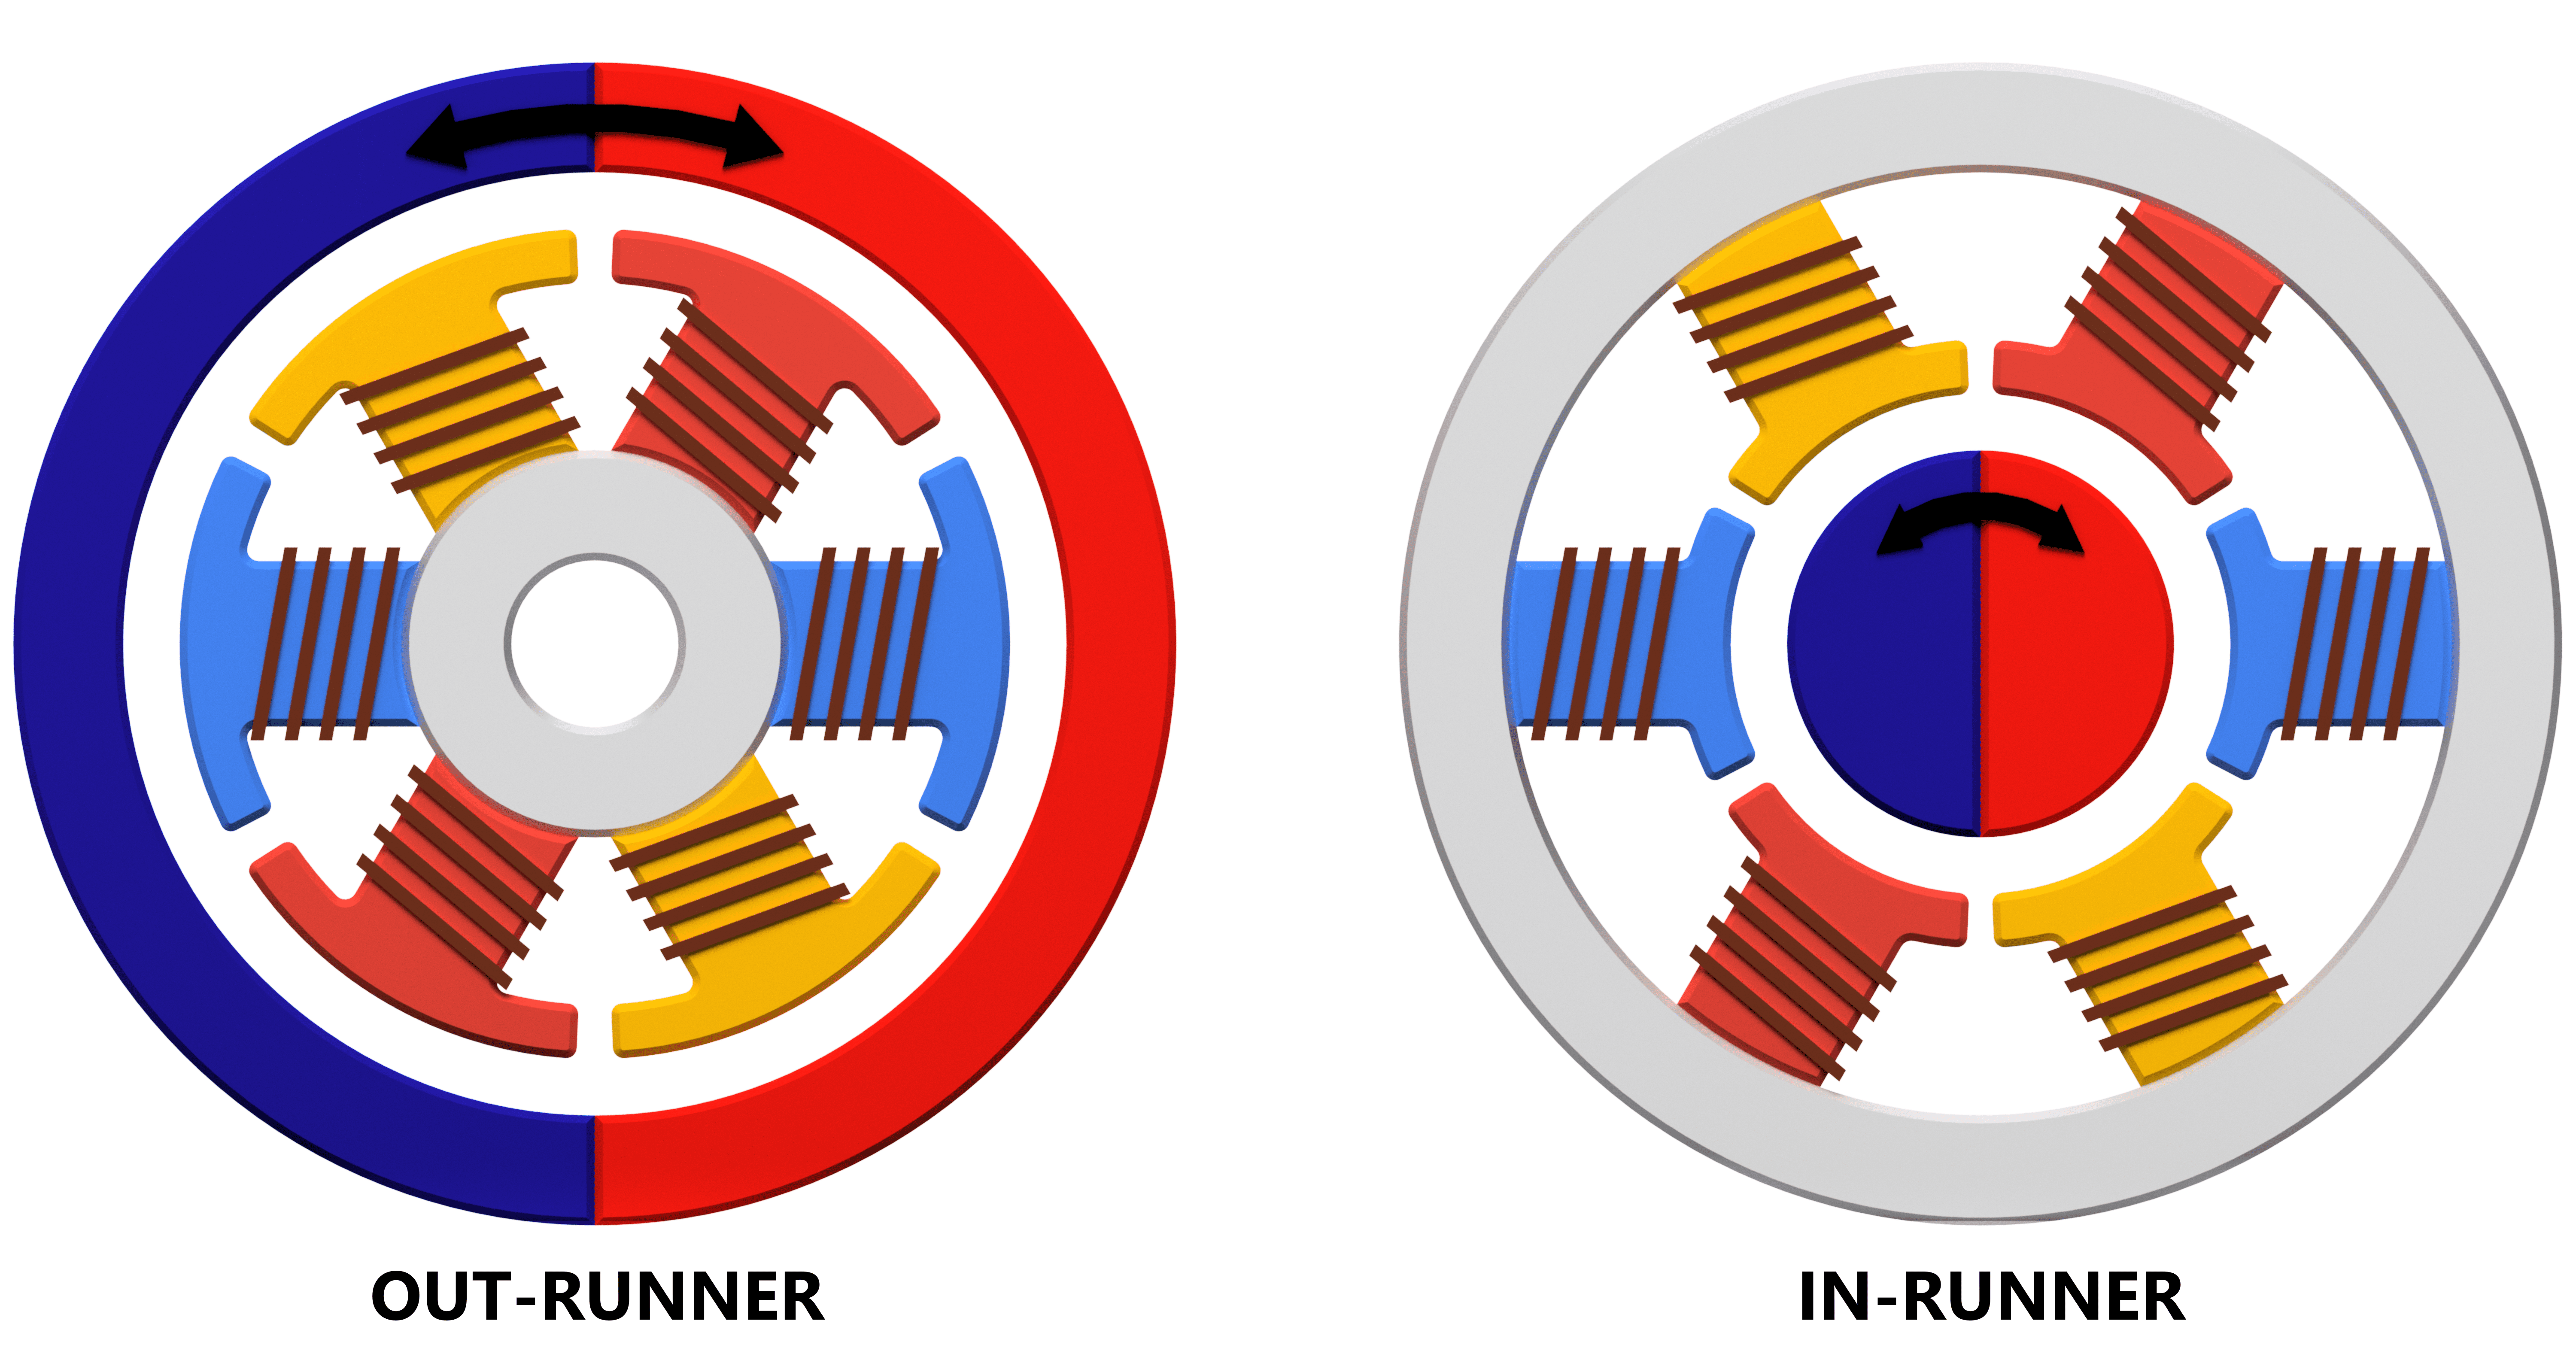
\includegraphics[width=0.6\textwidth]{imagenes/Motor/OUT_IN_BLDC_SF}
	\caption{Esquema de motores sin escobillas (\textit{BLDC}).}
	\label{fig:motor_sin_escobillas}
\end{figure}
\FloatBarrier

Similar a los motores trifásicos de corriente alterna, estos pueden tener configuraciones de bobinado en delta o estrella \cite{Millet2022}. Además, pueden presentar configuraciones \textit{in-runner}, donde los imanes están en el centro del eje con las bobinas en el exterior, o configuraciones \textit{out-runner} , donde los imanes se encuentran por fuera del motor, mientras que las bobinas están en el centro \cite{9774372}. Estos motores, al requerir una sincronización entre el campo magnético del estátor y el campo magnético del rotor, suelen utilizar encoders o sensores de efecto Hall para obtener información sobre la posición del eje, y de este modo, mantener una conmutación adecuada. No obstante, también es posible emplear técnicas \textit{sensorless} (sin sensor) para estimar la posición del rotor sin necesidad de sensores físicos. \cite{Gualtieri2018_STEP}

Los \textit{BLDC} se destacan por ofrecer una mayor densidad de potencia, mayor torque, mejor eficiencias y pueden llegar a velocidades mas altas. Sin embargo, al requerir de un controlador electrónico que se encargue de la conmutación para generar el movimiento del rotor, la complejidad y los costos asociados a su implementación son mayores. \cite{AN885}

\newpage
\subsection{Control Orientado de Campo (FOC)}
El control orientado de campo se basa en desacoplar el flujo electromagnético del par motor, permitiendo el control independiente de cada uno, aunque en este caso se realiza de forma indirecta, trabajando con las corrientes del estátor en ves de las variables en ves de las variables reales de flujo y par. Este desacoplamiento se logra mediante la transformación de las variables trifásicas del motor, que están en un marco de referencia estacionario \(ABC\), hacia un marco de referencia rotatorio \(dq\) que gira en sincronía con el rotor. \cite{power_conv_14}

\begin{figure}[ht]
	\centering
	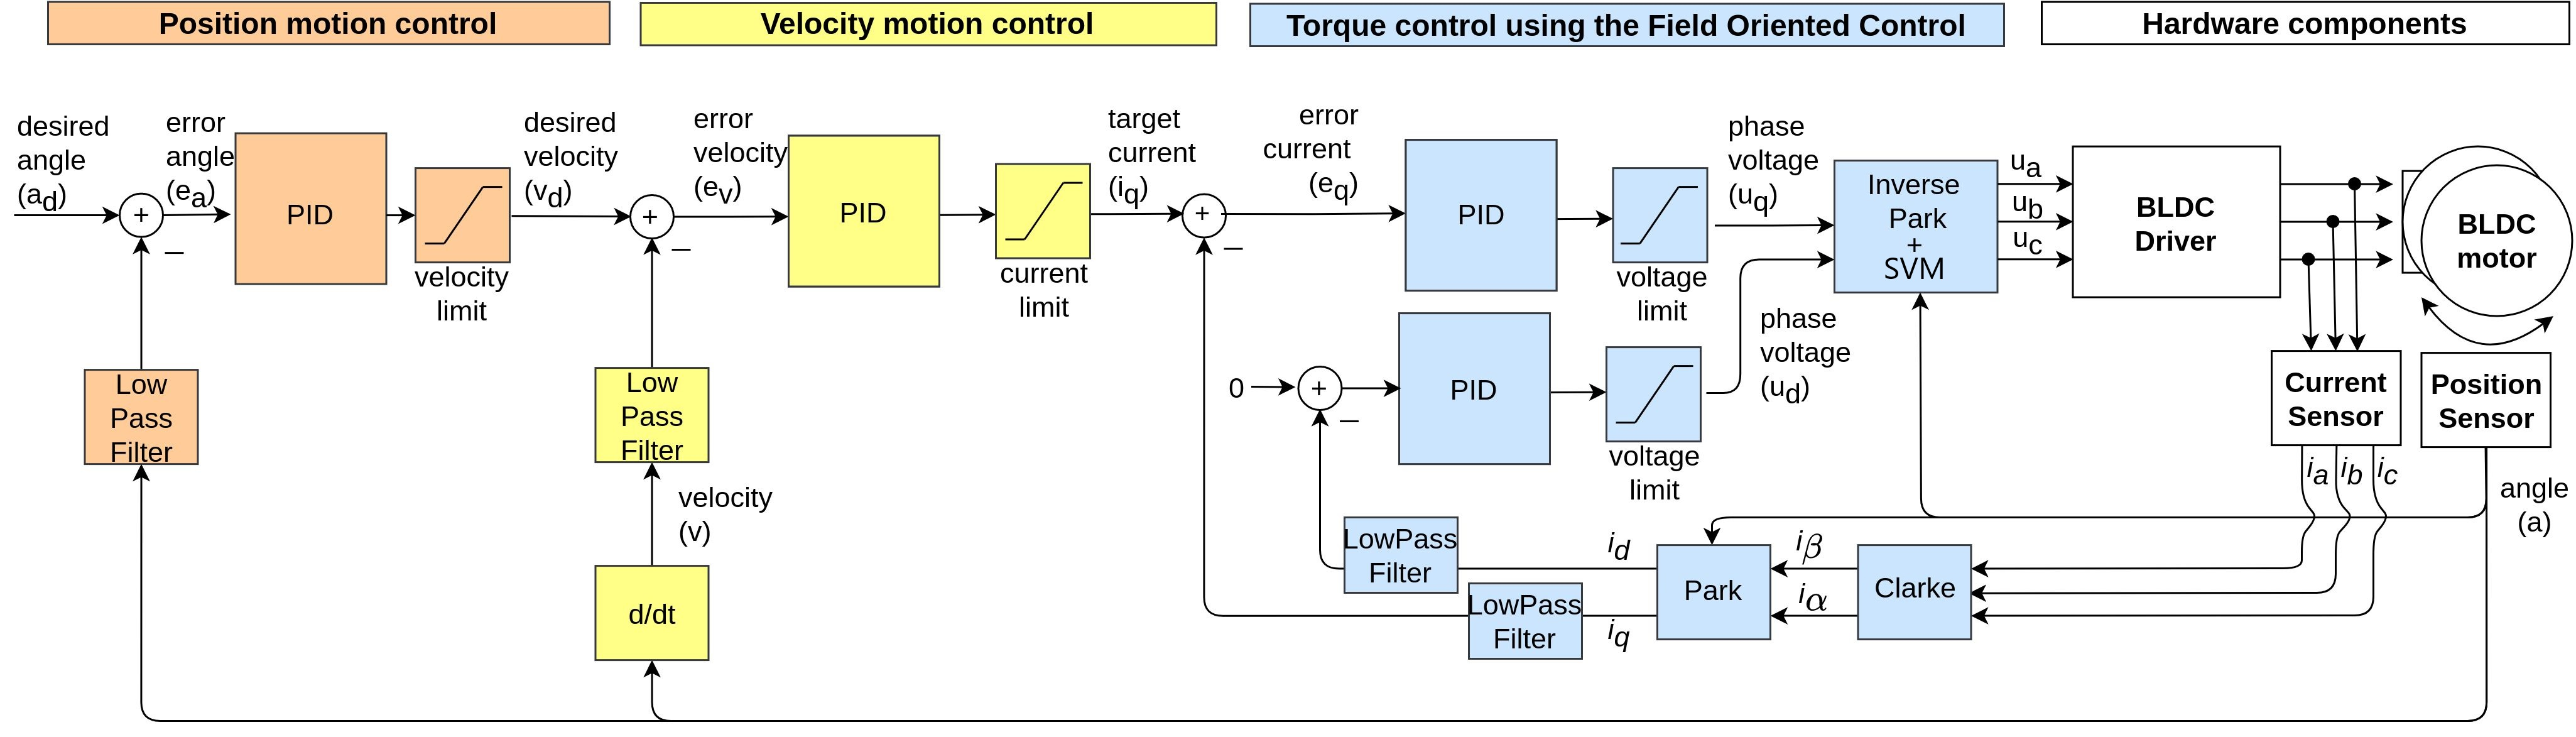
\includegraphics[width=0.9\textwidth]{imagenes/Diagramas/simpleFOC.jpg}
	\caption{Diagrama de flujo del control FOC.\cite{Skuric_SimpleFOC_A_Field_2022}}
	\label{fig:foc_transform}
\end{figure}
\FloatBarrier

La transformación entre los marcos de referencia se realiza aplicando la transformada de Clarke y la transformada de Park. De esta forma, las variables que presentan un comportamiento oscilatorio en el tiempo se convierten en variables de corriente continua, lo que permite emular, en cierta medida, el funcionamiento de un motor con escobillas a nivel del controlador. \cite{power_conv_14}

\subsection{Transformada de Clarke}
La transformada de Clarke convierte un sistema trifásico de corrientes \(ABC\) en un sistema bifásico \(\alpha\beta\), proyectando las corrientes en un sistema de coordenadas bidimensional estacionario. Esta transformación simplifica el análisis al reducir las tres corrientes de fase a dos componentes ortogonales, manteniendo la información esencial del sistema original. \cite{AN1078}


\begin{figure}[ht]
	\centering
	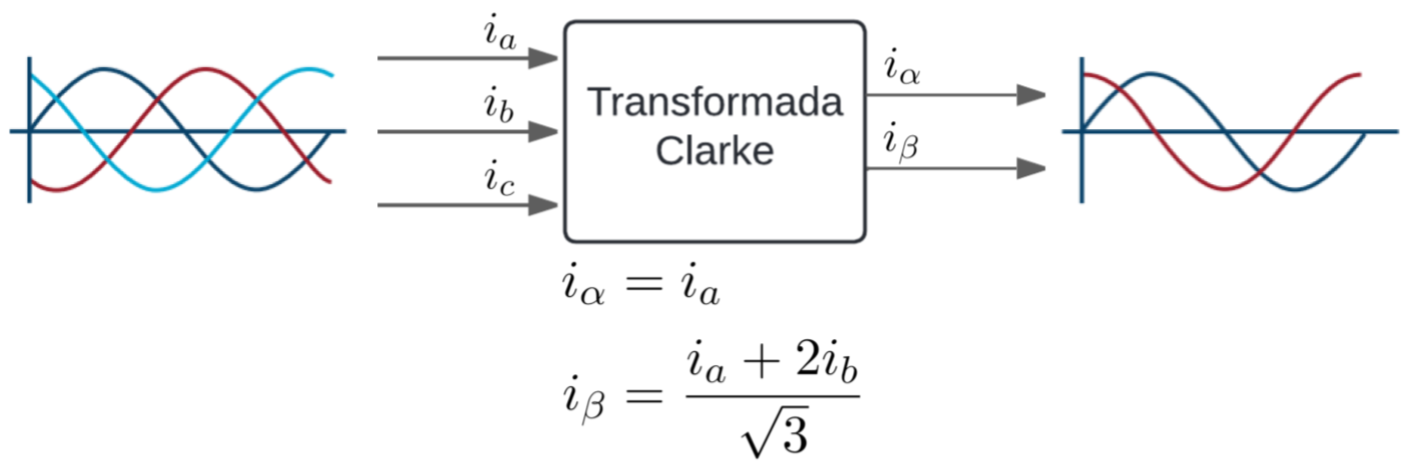
\includegraphics[width=0.8\textwidth]{imagenes/Diagramas/clarke.png}
	\caption{Esquema transformada de Clarke.}
	\label{fig:clarke_transform}
\end{figure}
\FloatBarrier

\newpage
\subsection{Transformada de Park}
La transformada de Park convierte el sistema en el marco de referencia estacionario \(\alpha\beta\) en el sistema en el marco de referencia rotatorio \(dq\) sincronizado con ángulo del rotor. \cite{AN1078}

\begin{figure}[ht]
	\centering
	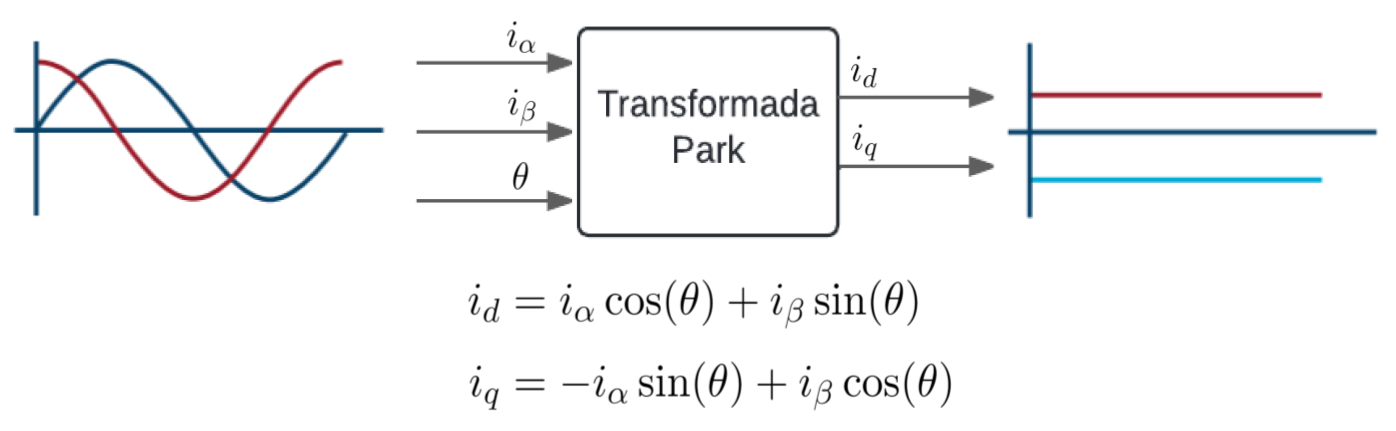
\includegraphics[width=0.8\textwidth]{imagenes/Diagramas/park.png}
	\caption{Esquema transformada de Park.}
\end{figure}
\FloatBarrier


\subsection{Transformada inversa de Park}
La transformada inversa de Park convierte el sistema en el marco de referencia rotatorio \(dq\) de vuelta al marco de referencia estacionario \(\alpha\beta\). \cite{AN1078}.

\begin{figure}[ht]
	\centering
	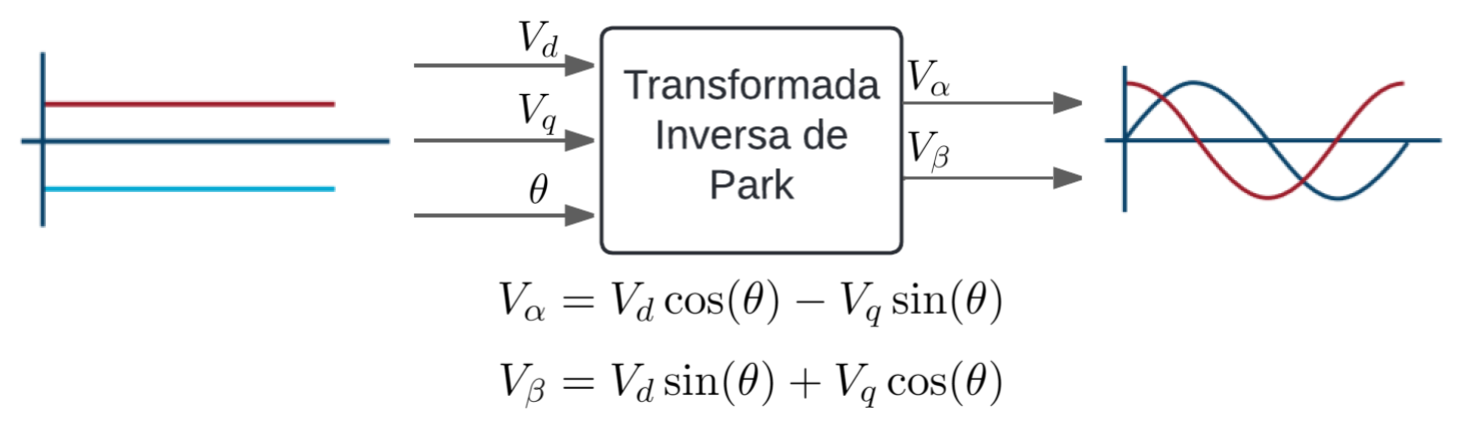
\includegraphics[width=0.8\textwidth]{imagenes/Diagramas/park_inv.png}
	\caption{Esquema transformada inversa de Park.}
\end{figure}
\FloatBarrier

\newpage
\subsection{Modulación de Espacio Vectorial (SVM)}
La Modulación por Vector Espacial (SVM) es una técnica utilizada para el control digital de inversores de voltaje. Representa los estados de conmutación del inversor como vectores de voltaje en el plano $\alpha$-$\beta$, formando un hexágono regular dividido en seis sectores o sextantes.

\begin{figure}[ht]
	\centering
	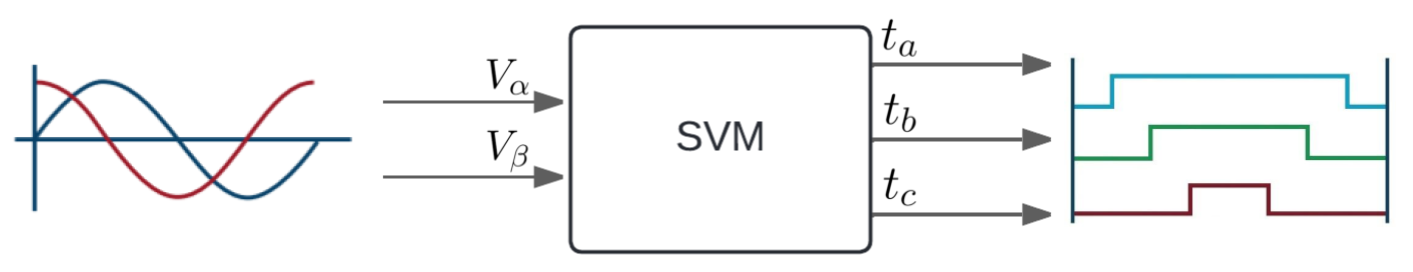
\includegraphics[width=0.6\textwidth]{imagenes/Diagramas/SVM.png}
	\caption{Esquema SVM.}
\end{figure}
\FloatBarrier

Esta técnica busca sintetizar el vector de referencia $\mathbf{V}_{\text{ref}}=(V_{\alpha},V_{\beta})$ mediante una suma ponderada de los vectores de voltaje adyacentes en el sextante donde se encuentre, logrando una aproximación más \href{https://www.youtube.com/watch?v=NY0ffyEu6uo}{precisa} de la señal deseada.

\begin{figure}[ht]
	\centering
	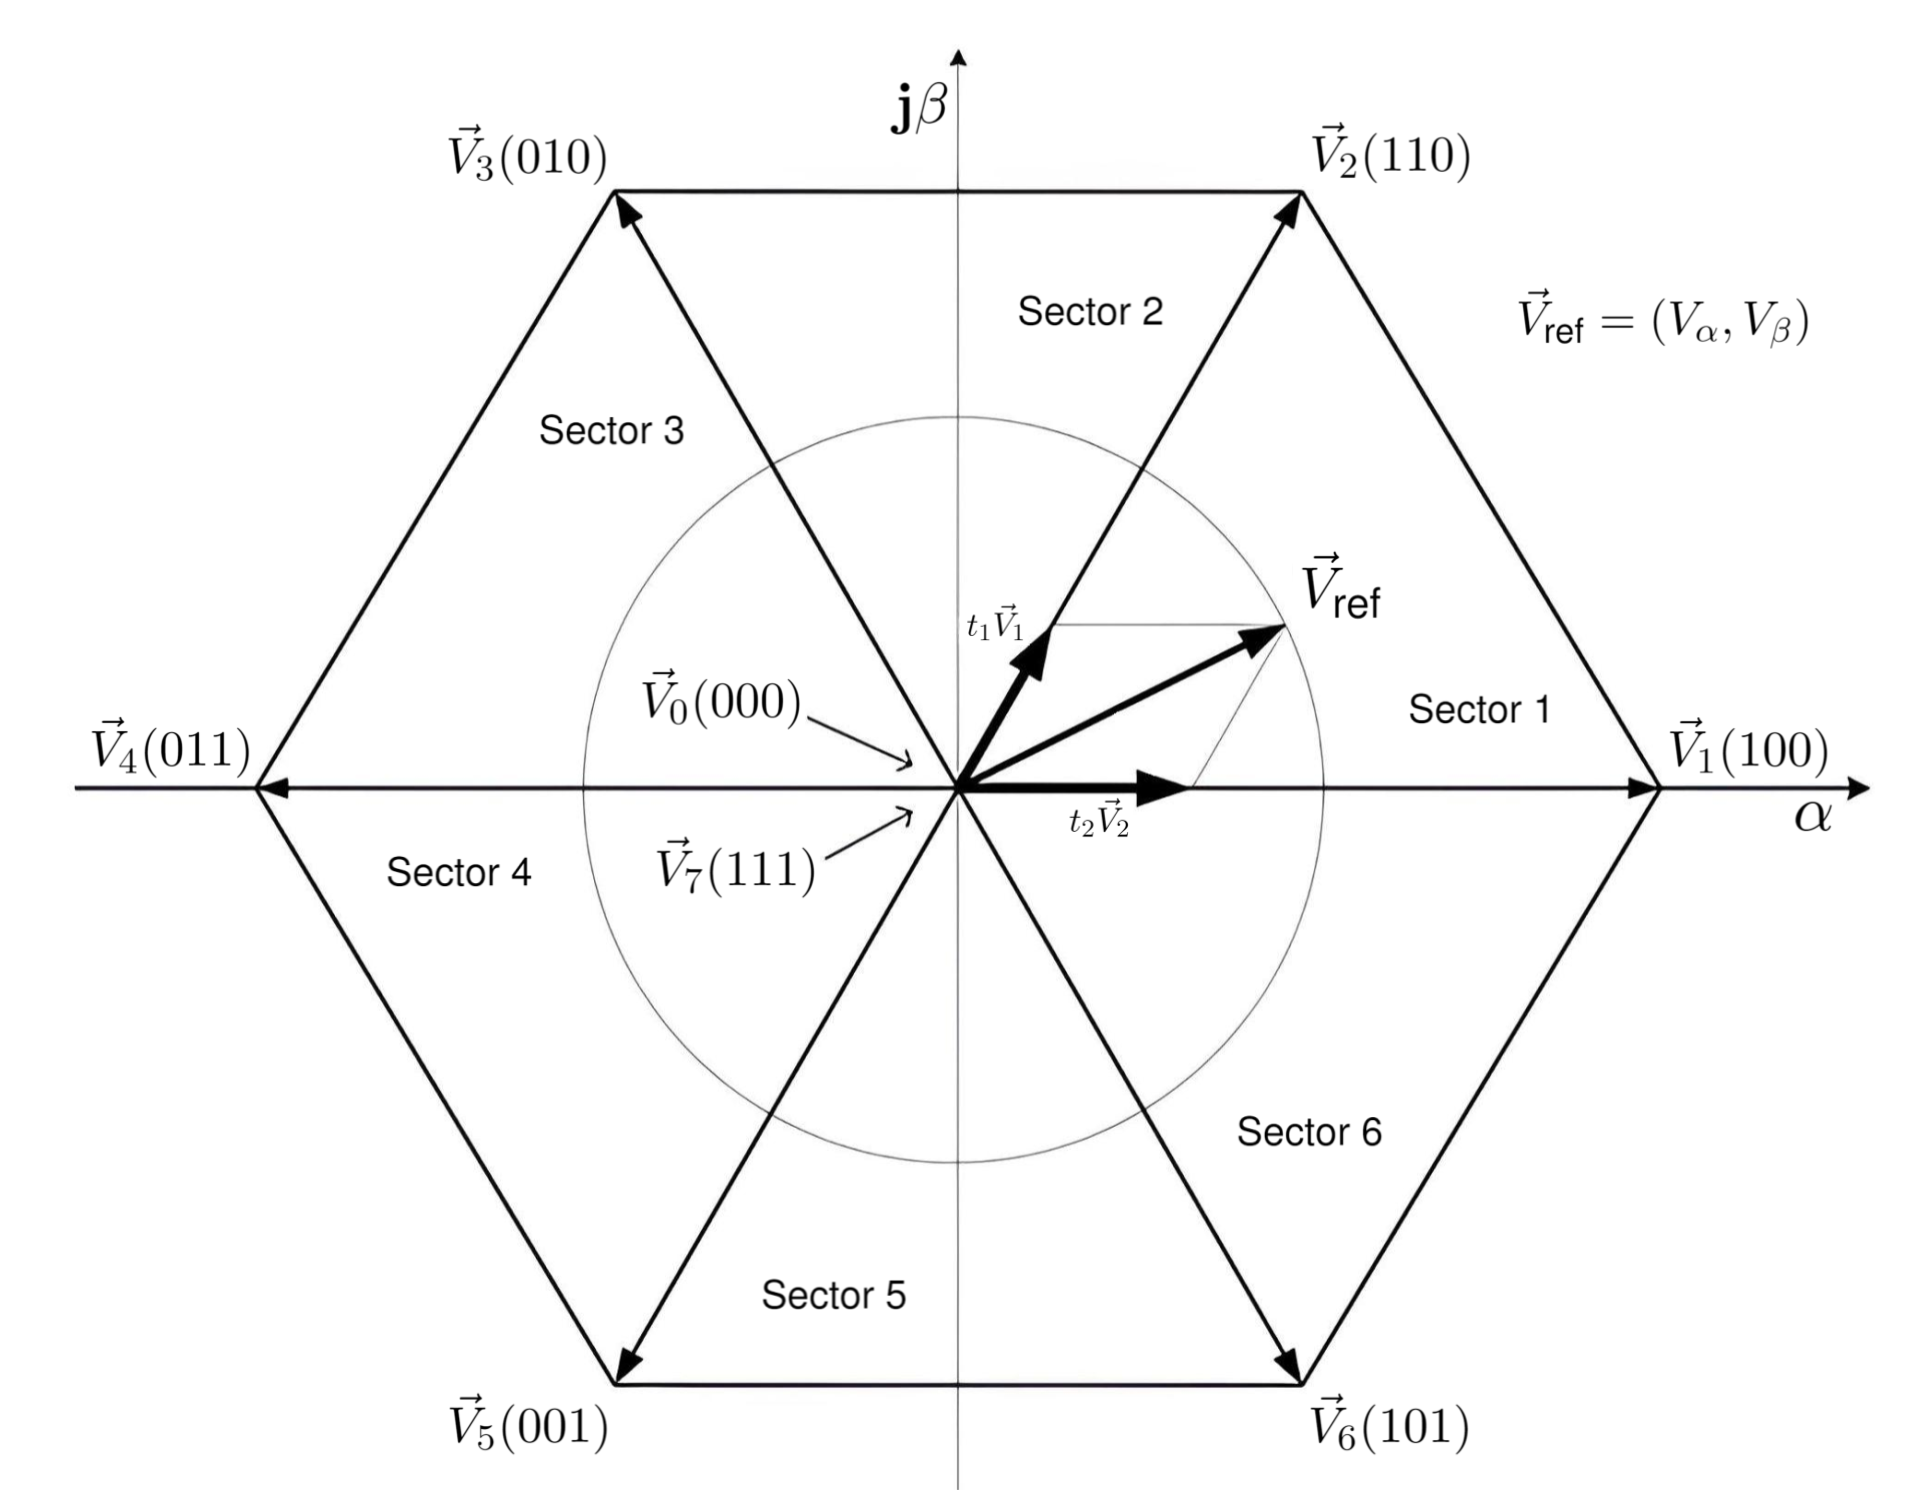
\includegraphics[width=0.5\textwidth]{imagenes/Diagramas/sectantes.png}
	\caption{Sextantes en SVM.}
\end{figure}
\FloatBarrier

Se utiliza un patrón de activación específico que permite minimizar la frecuencia de conmutación de los transistores, aprovechando estados redundantes para reducir las pérdidas asociadas a la conmutación y mejorar la eficiencia del sistema. \cite{power_conv_06}

\begin{table}[htbp]
	\centering
	\caption{Secuencia de Conmutación en SVM}
	\begin{tabular}{ c c c c c c c c }
		\hline
		\textbf{Sector} & \textbf{1}       & \textbf{2}       & \textbf{3}       & \textbf{4}       & \textbf{5}       & \textbf{6}       & \textbf{7}       \\
		\hline
		I               & $\vec{V}_0(000)$ & $\vec{V}_1(100)$ & $\vec{V}_2(110)$ & $\vec{V}_7(111)$ & $\vec{V}_2(110)$ & $\vec{V}_1(100)$ & $\vec{V}_0(000)$ \\
		II              & $\vec{V}_0(000)$ & $\vec{V}_3(010)$ & $\vec{V}_2(110)$ & $\vec{V}_7(111)$ & $\vec{V}_2(110)$ & $\vec{V}_3(010)$ & $\vec{V}_0(000)$ \\
		III             & $\vec{V}_0(000)$ & $\vec{V}_3(010)$ & $\vec{V}_4(011)$ & $\vec{V}_7(111)$ & $\vec{V}_4(011)$ & $\vec{V}_3(010)$ & $\vec{V}_0(000)$ \\
		IV              & $\vec{V}_0(000)$ & $\vec{V}_5(001)$ & $\vec{V}_4(011)$ & $\vec{V}_7(111)$ & $\vec{V}_4(011)$ & $\vec{V}_5(001)$ & $\vec{V}_0(000)$ \\
		V               & $\vec{V}_0(000)$ & $\vec{V}_5(001)$ & $\vec{V}_6(101)$ & $\vec{V}_7(111)$ & $\vec{V}_6(101)$ & $\vec{V}_5(001)$ & $\vec{V}_0(000)$ \\
		VI              & $\vec{V}_0(000)$ & $\vec{V}_1(100)$ & $\vec{V}_6(101)$ & $\vec{V}_7(111)$ & $\vec{V}_6(101)$ & $\vec{V}_1(100)$ & $\vec{V}_0(000)$ \\
		\hline
	\end{tabular}
\end{table}
%cuarto párrafo

\newpage
\section{Motivación}
Este proyecto nace de la necesidad de un controlador para motores brushless adecuado para su uso en robots de competencia en la categoría de robot sumo autónomo. En esta categoría, este tipo de motores no son normalmente utilizados debido a las limitaciones de los controladores comerciales y los riesgos que conlleva la sobrecarga de los motores en periodos cortos de acción, ya que los \href{https://www.youtube.com/watch?v=SmDZmGU08BM}{controladores comerciales} no están pensados para esto.

\section{Objetivos}
\subsection{Objetivo General}
Implementar un controlador de tipo FOC (Control de Campo Orientado) para motores brushless con encoder, utilizando un microcontrolador STM32, que sirva de base para un driver especializado en la robótica competitiva.

\subsection{Objetivos Específicos}
\begin{itemize}
	\item Estudiar los principios del Control de Campo Orientado (FOC) y la modulación de espacio vectorial (SVM) para aplicarlos en el diseñó del controlador.
	\item Diseñar el hardware para el controlador FOC, con los componentes mínimos necesarios para validar el funcionamiento.
	\item Configurar y programar el microcontrolador para el algoritmo FOC, utilizando las librerías HAL de STM32
	\item Validar el funcionamiento del controlador y proponer posibles mejoras para su aplicación en robótica competitiva.
\end{itemize}

\newpage
\subsection{Alcances}
\begin{itemize}
	\item Se configurará el microcontrolador utilizando STM32CubeMX.
	\item Se implementará el controlador de velocidad y corriente.
	\item No se implementará el control de posición.
	\item Se programará el firmware utilizando VScode y el lenguaje C.
	\item El firmware se compilará utilizando un makefile y GCC, junto con la extensión STM32 for VScode.
	\item Se cargará el firmware utilizando STM32CubeProgrammer y ST-link.
	\item Se diseñará la PCB en Eagle.
	\item Se diseñarán las piezas adicionales en Autodesk Inventor, para su posterior fabricación mediante impresión 3D.
	\item La PCB se fabricará y semi ensamblará utilizando \href{https://www.youtube.com/watch?v=riT4nl0T8_M}{JLCPCB}.
	\item Se obtendrán datos detallados durante el tiempo de ejecución.
	\item Los datos se graficarán utilizando Plotly en Python.
	\item Se identificarán posibles mejoras.
\end{itemize}

\chapter{Hardware}
\section{Introducción}
Este capítulo busca documentar el desarrollo e implementación de todo el hardware y electrónica necesaria para el controlador FOC, partiendo por la revisión los parámetros principales y componentes utilizados para finalmente revisar a grandes rasgos el diseñó de la placa controladora.


\begin{figure}[ht]
	\centering
	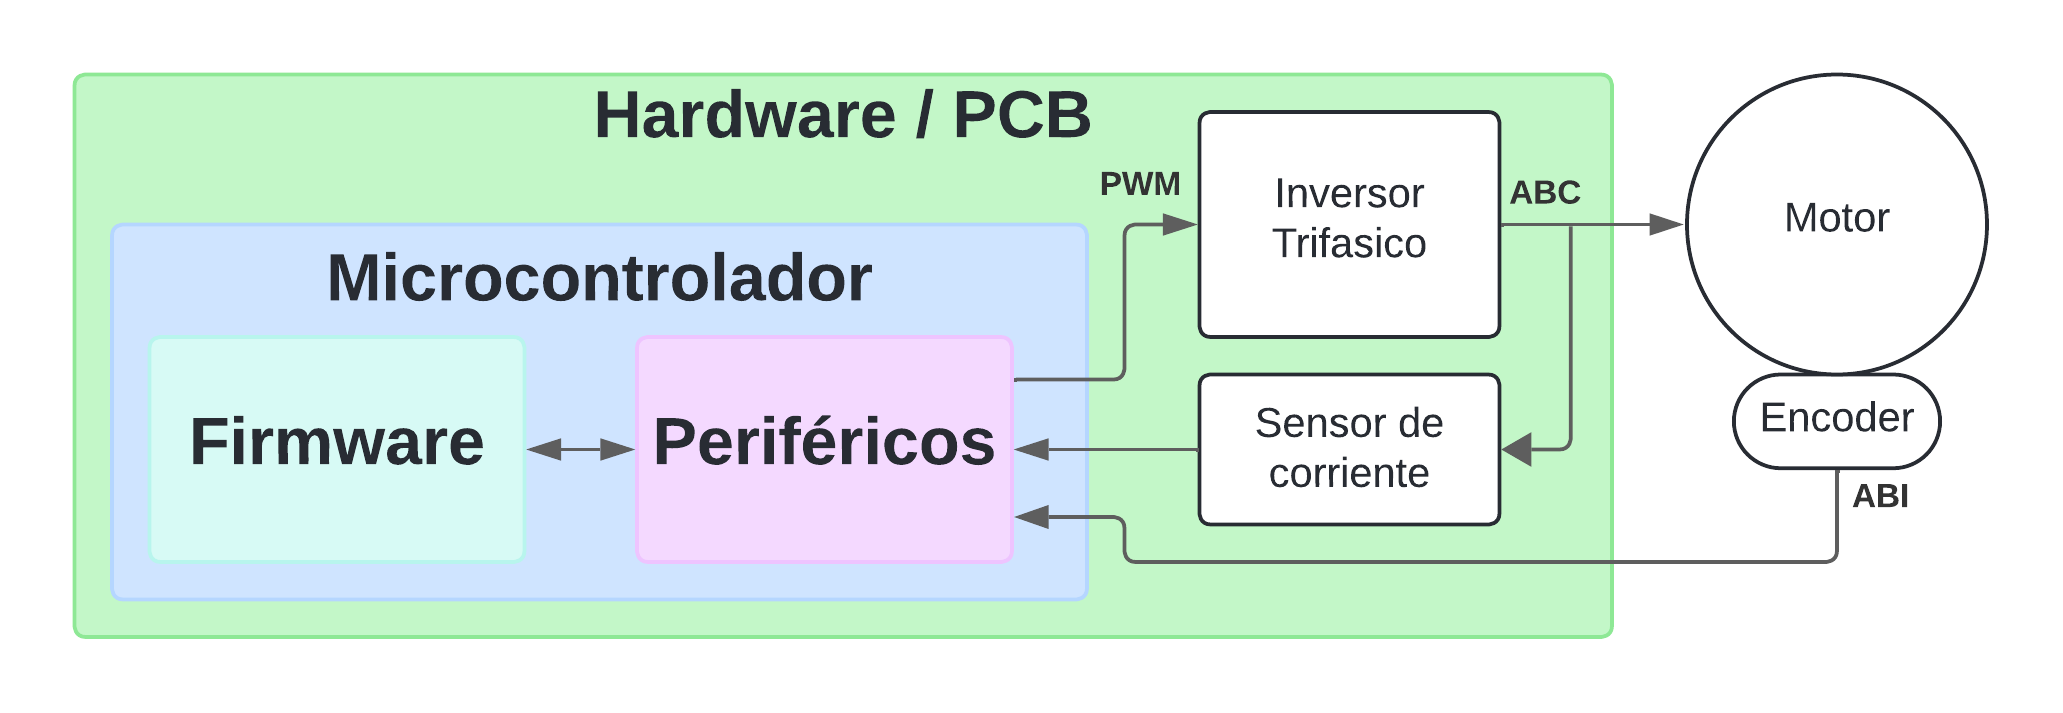
\includegraphics[width=0.76\textwidth]{imagenes/Diagramas/Diagramas - ultra resumen.png}
	\caption{Diagrama Resumido del sistema.}
	\label{flujo_resumen}
\end{figure}
\FloatBarrier

En la Figura \ref{flujo_resumen} se muestra una vista general de la interacción entre los bloques principales del controlador. El microcontrolador, programado con el firmware que utiliza los periféricos para generar las señales PWM necesarias para conducir el inversor trifásico encargado de suministrar la corriente al motor, adquirir las mediciones de corriente de las fases y la posición del rotor a través del encoder. De esta manera cerrando el lazo de control FOC.

\newpage
\section{Desarrollo del hardware}
En esta sección se busca mostrar, a grandes rasgos, los componentes esenciales utilizados en el controlador, tal como se ilustra en la Figura \ref{flujo_resumen_hardware}. El \emph{hardware} está compuesto por un inversor trifásico con MOSFETs, controladores de puerta (\emph{gate drivers}), resistencias \emph{shunt} para la medición de corriente y un motor \emph{brushless} con \emph{encoder}. El regulador de voltaje a 12 V suministra la alimentación necesaria a los controladores de puerta, mientras que la batería provee la potencia principal para el puente MOSFET.

\begin{figure}[ht]
	\centering
	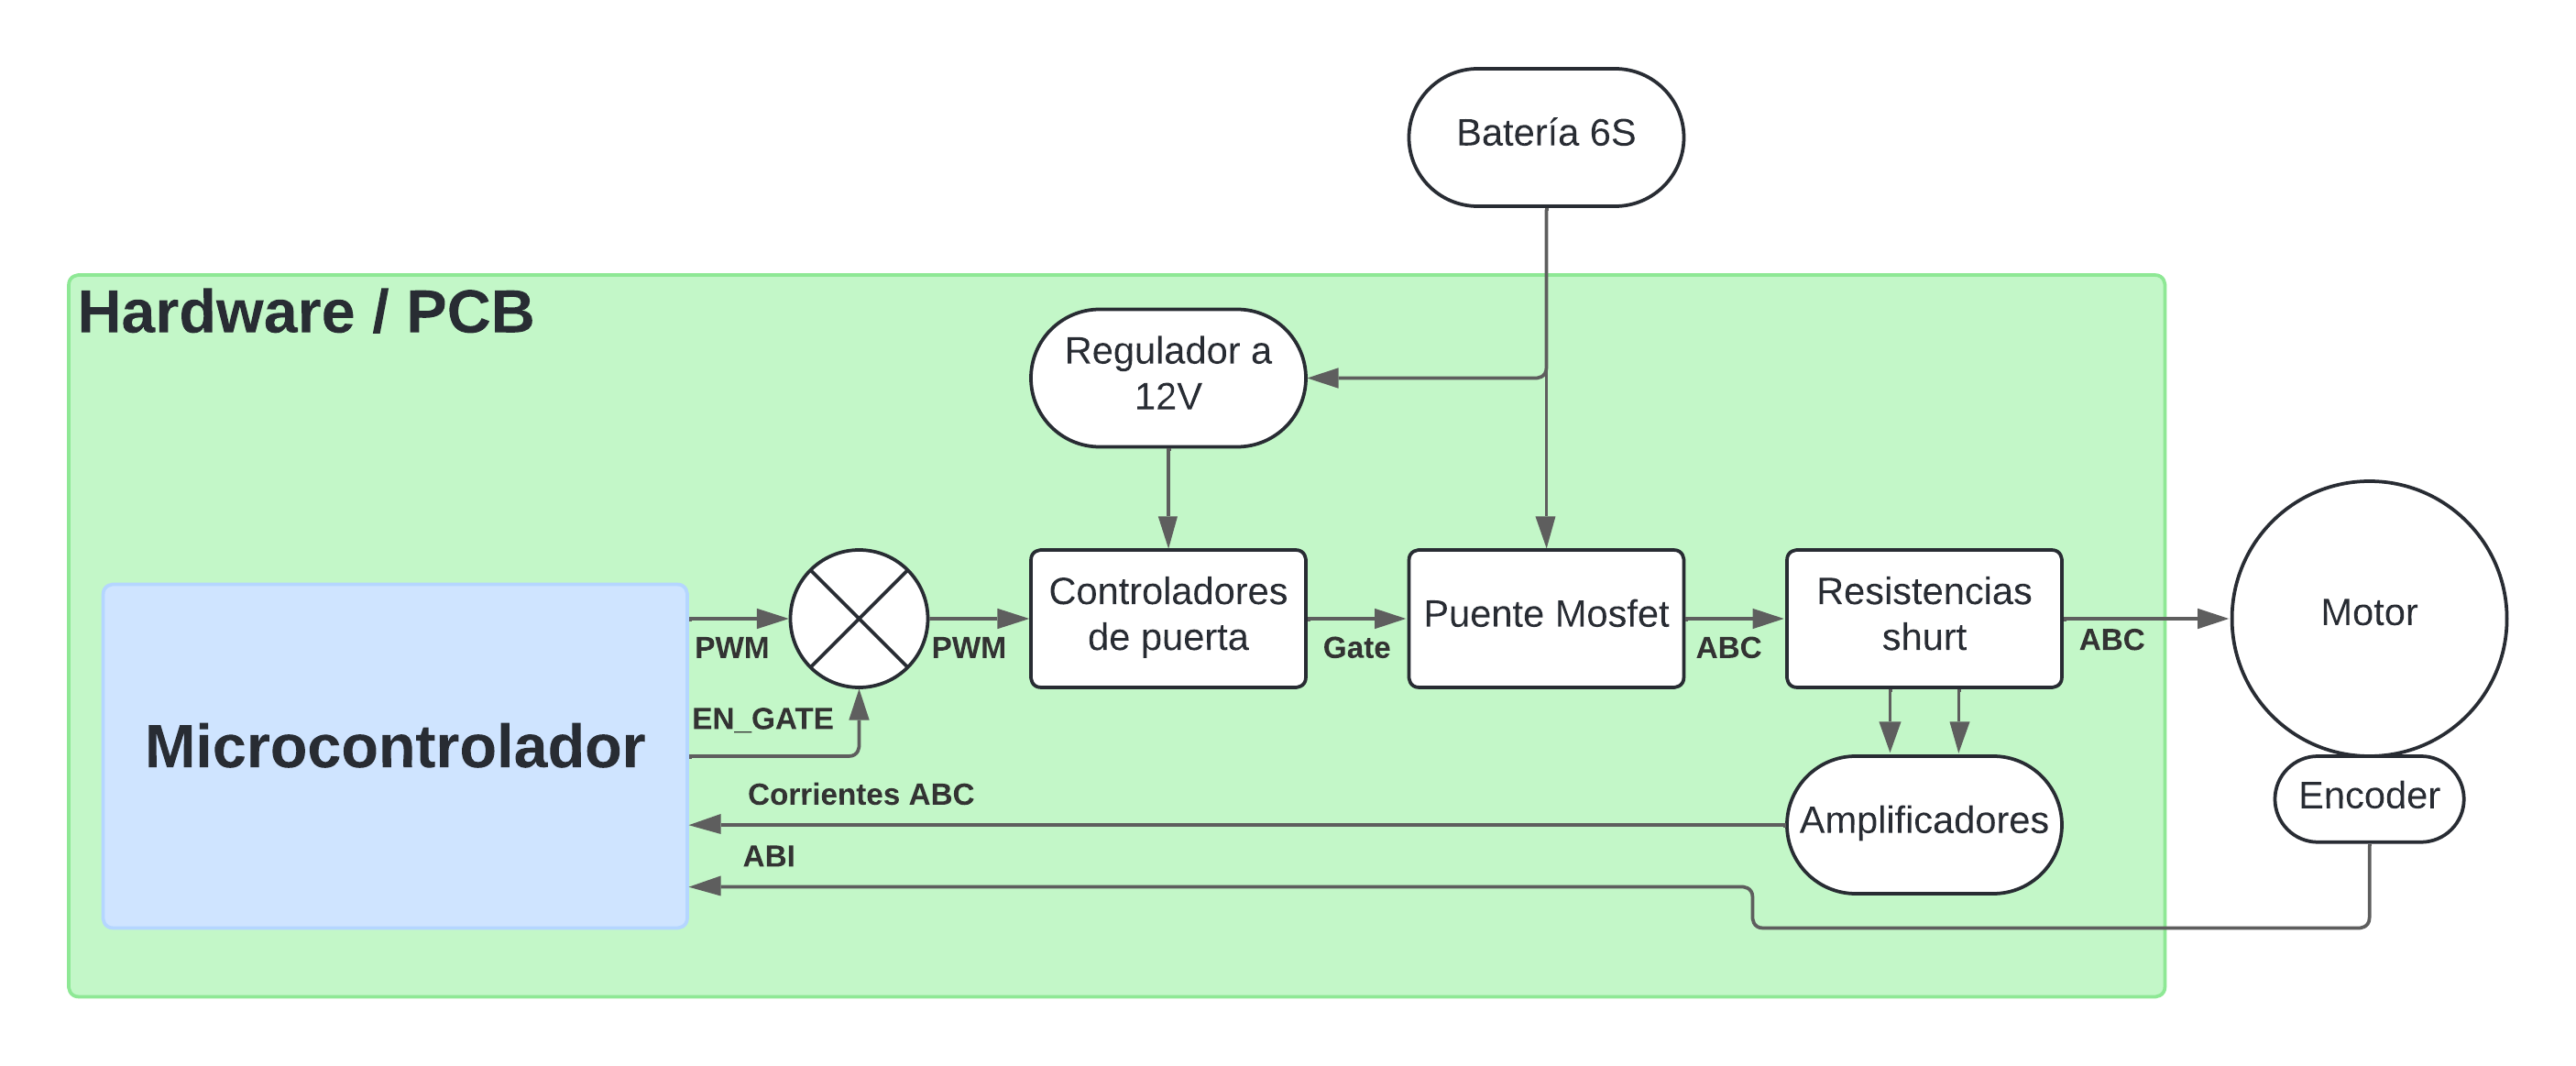
\includegraphics[width=0.76\textwidth]{imagenes/Diagramas/Diagramas - resumen hardware.png}
	\caption{Diagrama Resumido del hardware.}
	\label{flujo_resumen_hardware}
\end{figure}
\FloatBarrier

\subsection{Motor}

El punto de partida es la selección del motor, que define parámetros cruciales como corriente máxima, voltaje nominal y la velocidad máxima (\emph{Kv}). Estos influyen directamente en la elección de los MOSFETs y resistencias \emph{shunt} para manejar la corriente requerida.

\begin{figure}[ht]
	\centering
	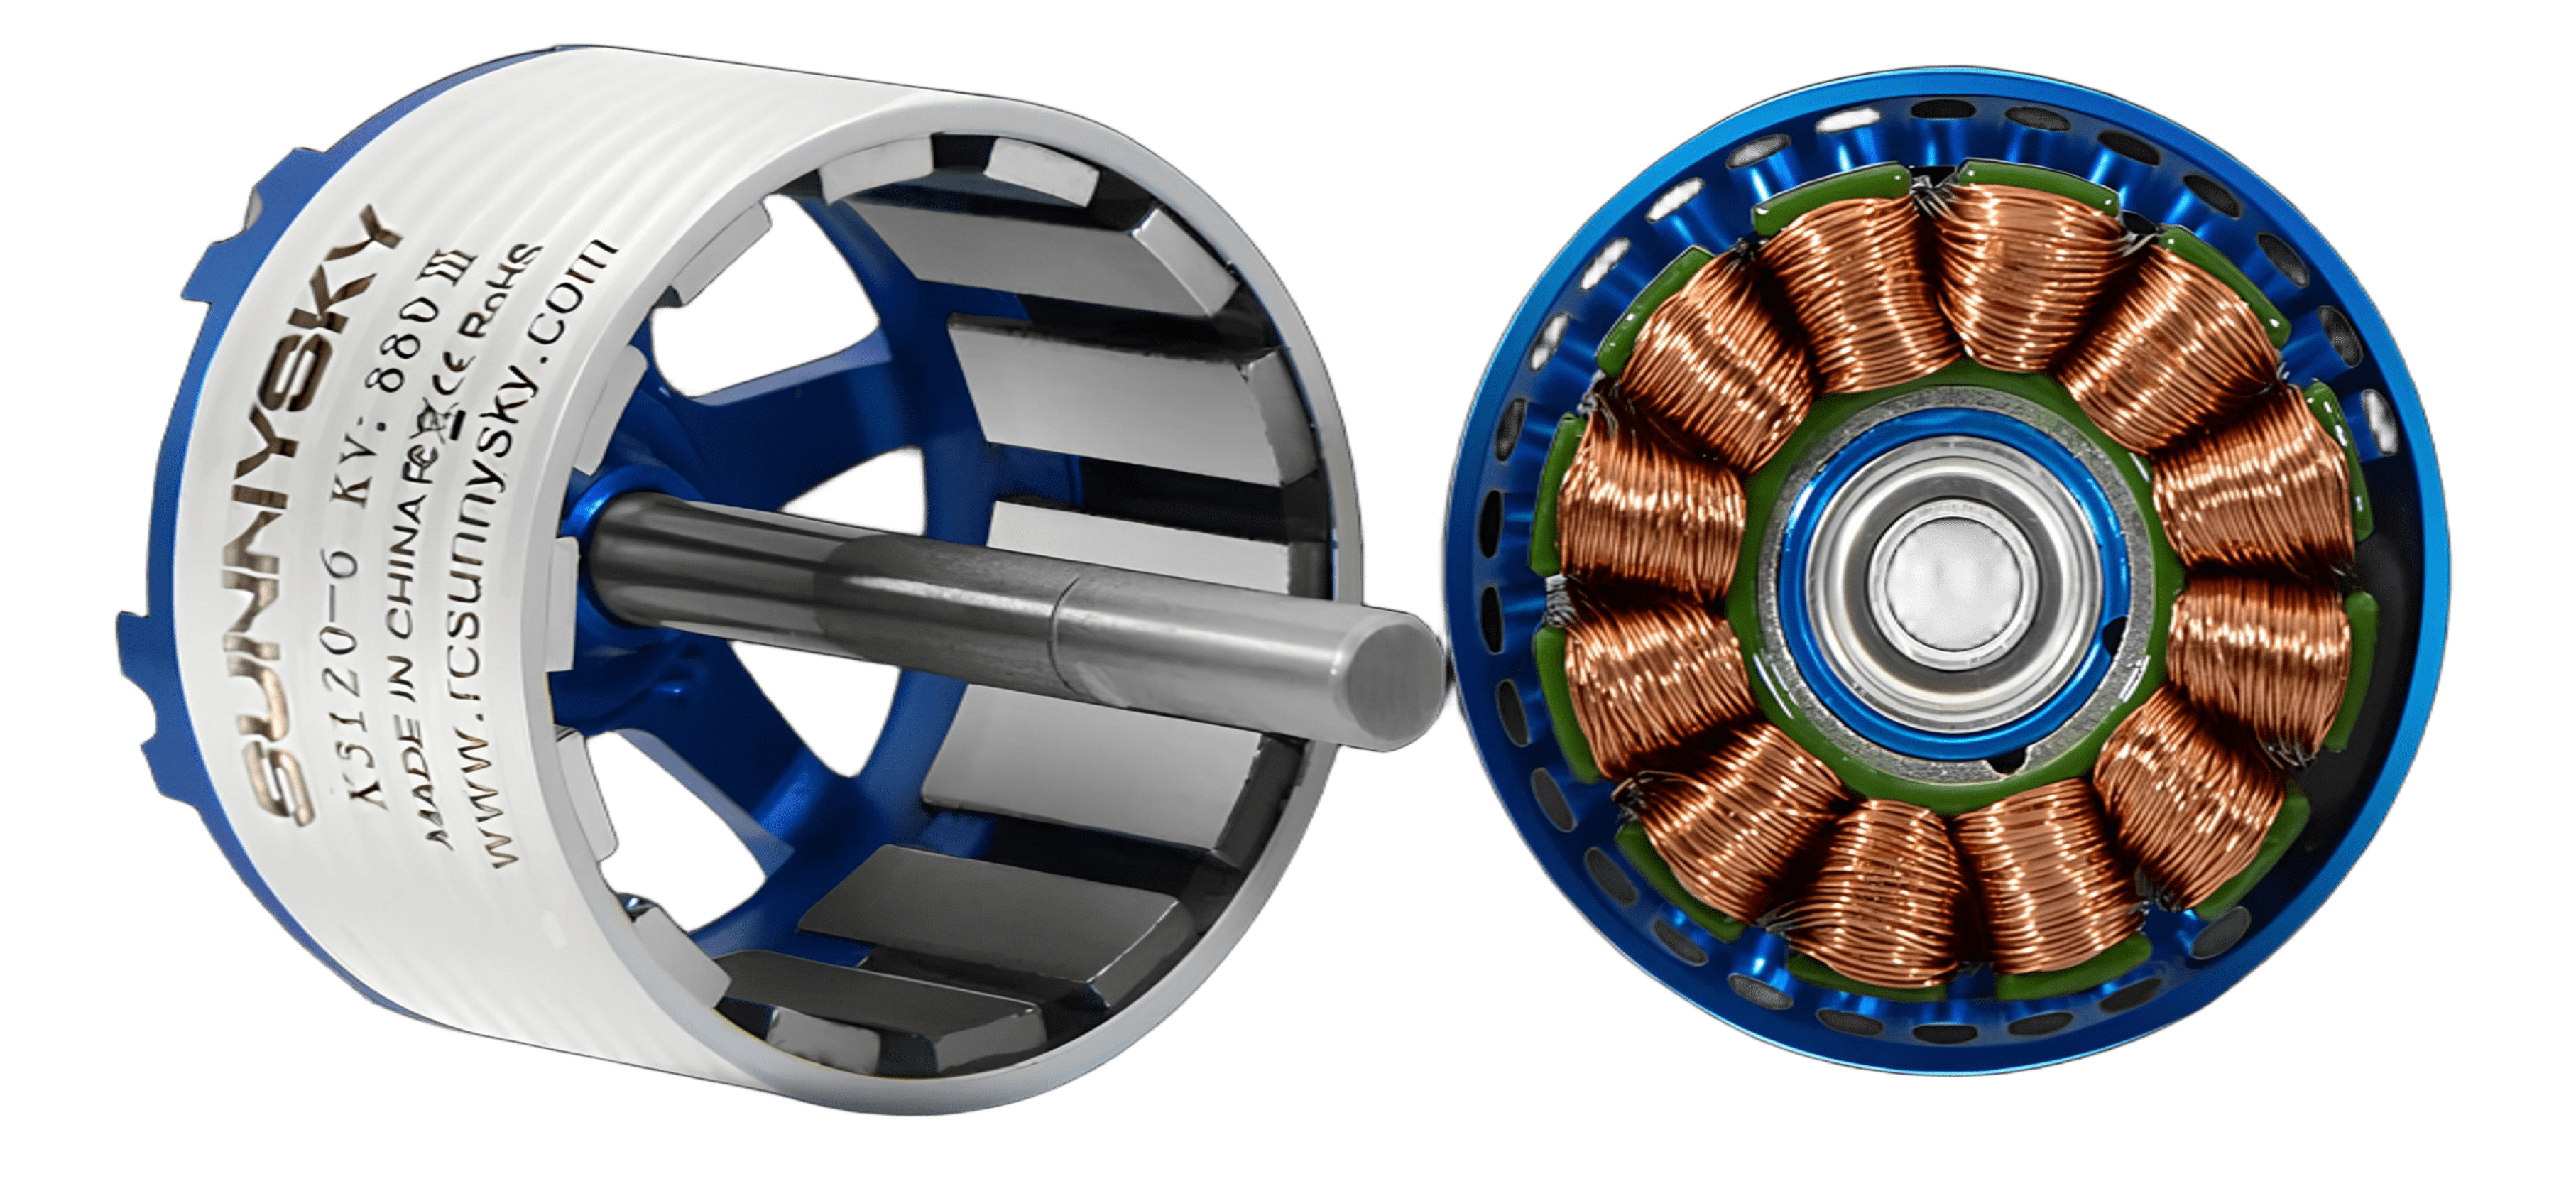
\includegraphics[width=0.8\textwidth]{imagenes/Motor/X3120.png}
	\caption{SunnySky X3120 V3.}
	\label{X3120}
\end{figure}
\FloatBarrier
\newpage
Se ha optado por utilizar el motor \textbf{SunnySky X3120 V3} de 585Kv para el diseñó del controlador debido a su disponibilidad inmediata. Este es un motor principalmente orientado al uso en drones de tipo aeroplano, pero su gran potencia y bajo peso lo hace ideal para su uso en robots sumo.

\begin{table}[h!]
	\centering
	\caption{Características del motor SunnySky X3120 V3 585Kv}
	\begin{tabular}{l l}
		\hline
		\textbf{Propiedad}               & \textbf{Valor} \\
		\hline
		Número de polos del rotor        & 14             \\
		Número de ranuras del estátor    & 12             \\
		Máxima celda Lipo                & 6S (22.2 V)    \\
		Constante de velocidad del motor & 585 $K_v$      \\
		Resistencia del motor            & 43.5 m$\Omega$ \\
		Corriente continua máxima        & 65 A/30 s      \\
		Potencia continua máxima         & 1625 W         \\
		Corriente en vacío               & 1.0 A/10 V     \\
		\hline
	\end{tabular}
\end{table}
\FloatBarrier

Algunos de los parámetros mas relevantes para el diseñó del hardware son el voltaje nominal, que esta marcado como 6S (celdas de lipo), las celdas de lipo varían su voltaje en función de su carga, teniendo un voltaje mínimo de 3V, nominal de 3.7V y máximo de 4.2V, por esto, una batería de 6 celdas en serie corresponde a un voltaje mínimo de 18V, nominal de 22.2V y máximo de 25.2V. otro parámetro importante es la corriente continua máxima de 65A.

\newpage
\subsection{Encoder}

El encoder es el encargado de proveer la información sobre la posición angular del rotor en el motor, se utilizó el encoder magnético AS5047P, el cual utiliza un imán especial con una polarización diametral en el eje del motor y un arreglo de sensores HAL internos, para poder medir e interpretar la posición angular del imán.

\begin{figure}[ht]
	\centering
	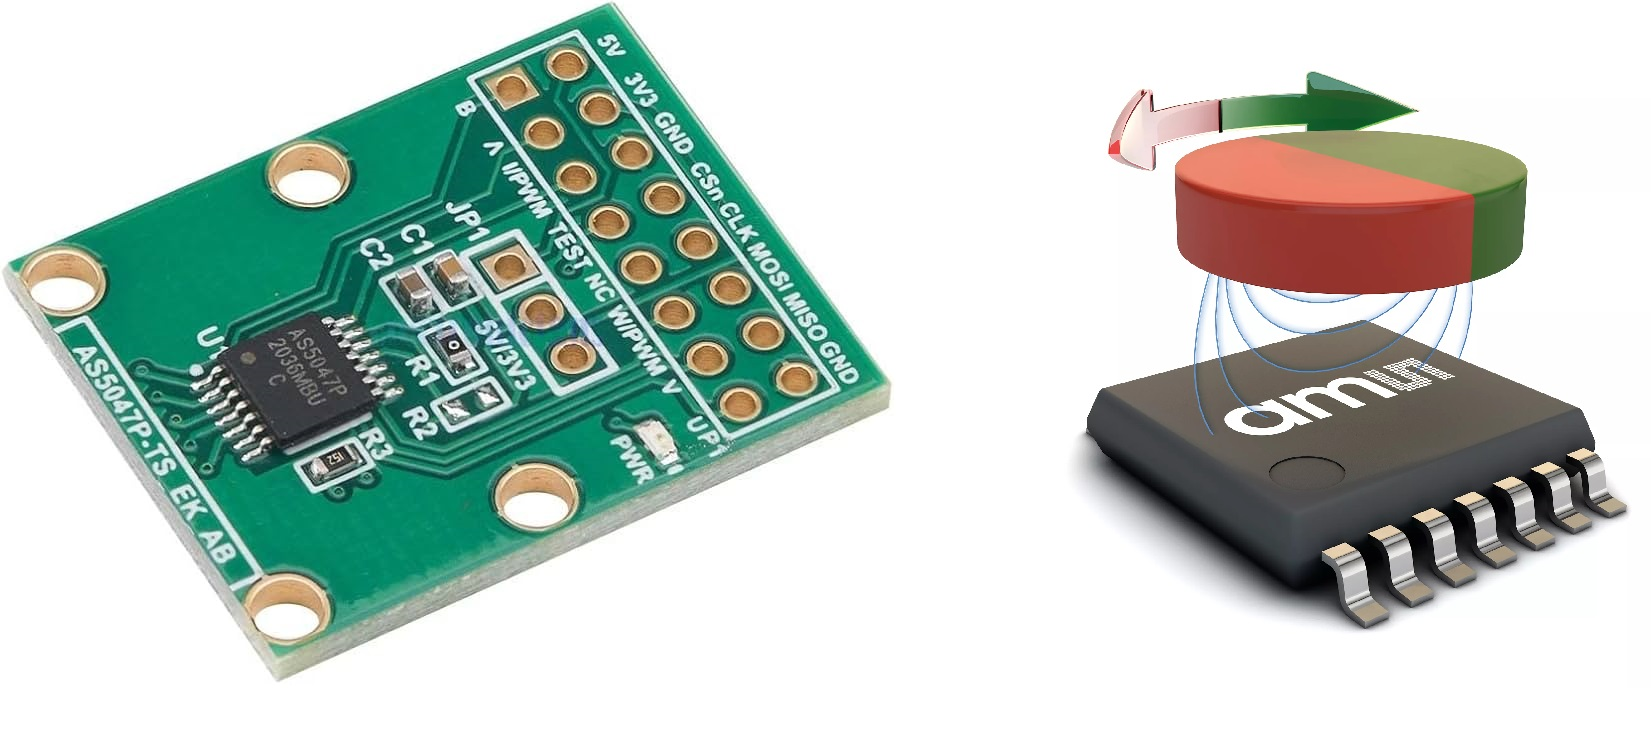
\includegraphics[width=0.6\textwidth]{imagenes/Motor/AS5047P.jpg}
	\caption{AS5047P.}
	\label{AS5047P}
\end{figure}
\FloatBarrier

En esencia este es un encoder absoluto que funciona principalmente a traves de una comunicación SPI, pero opcionalmente incorpora una salida que imita el comportamiento de un encoder incremental con señal index también conocidos como ABI o ABZ por sus señales, los microcontroladores STM32 incorporan periféricos que pueden trabajar de forma nativa con estas señales sin mayor intervención del procesador, lo que simplifica en gran medida su implementación en comparación con el uso de SPI, aun que en consecuencia se pierden las capacidades de encoder absoluto.

\begin{table}[h!]
	\centering
	\caption{Características del encoder AS5047P}
	\begin{tabular}{l c c c l}
		\hline
		\textbf{Parámetro}            & \textbf{Mín} & \textbf{Típ} & \textbf{Máx} & \textbf{Unidad}      \\
		\hline
		Tensión de alimentación (LDO) & 4.5          & 5.0          & 5.5          & $\mathrm{V}$         \\
		Tensión de alimentación       & 3.0          & 3.3          & 3.6          & $\mathrm{V}$         \\
		Corriente de suministro       &              & 15           &              & $\mathrm{mA}$        \\
		Velocidad máxima              &              &              & 28000        & $\mathrm{RPM}$       \\
		Resolución del núcleo         &              & 14           &              & $\mathrm{bits}$      \\
		Resolución ABI                & 25           & 512          & 1024         & $\mathrm{PPR}$       \\
		Resolución ABI (X4)           & 100          & 2048         & 4096         & $\mathrm{Pasos/rev}$ \\
		\hline
	\end{tabular}
\end{table}
\FloatBarrier

\newpage
\subsection{Conjunto motor encoder}
El encoder requiere estar fijo junto al motor y centrado respecto al eje del motor, por esto se diseñó en Autodesk Inventor y posteriormente se fabricó con impresión 3D, una montura hecha a la medida para el conjunto motor-encoder.

\begin{figure}[ht]
	\centering
	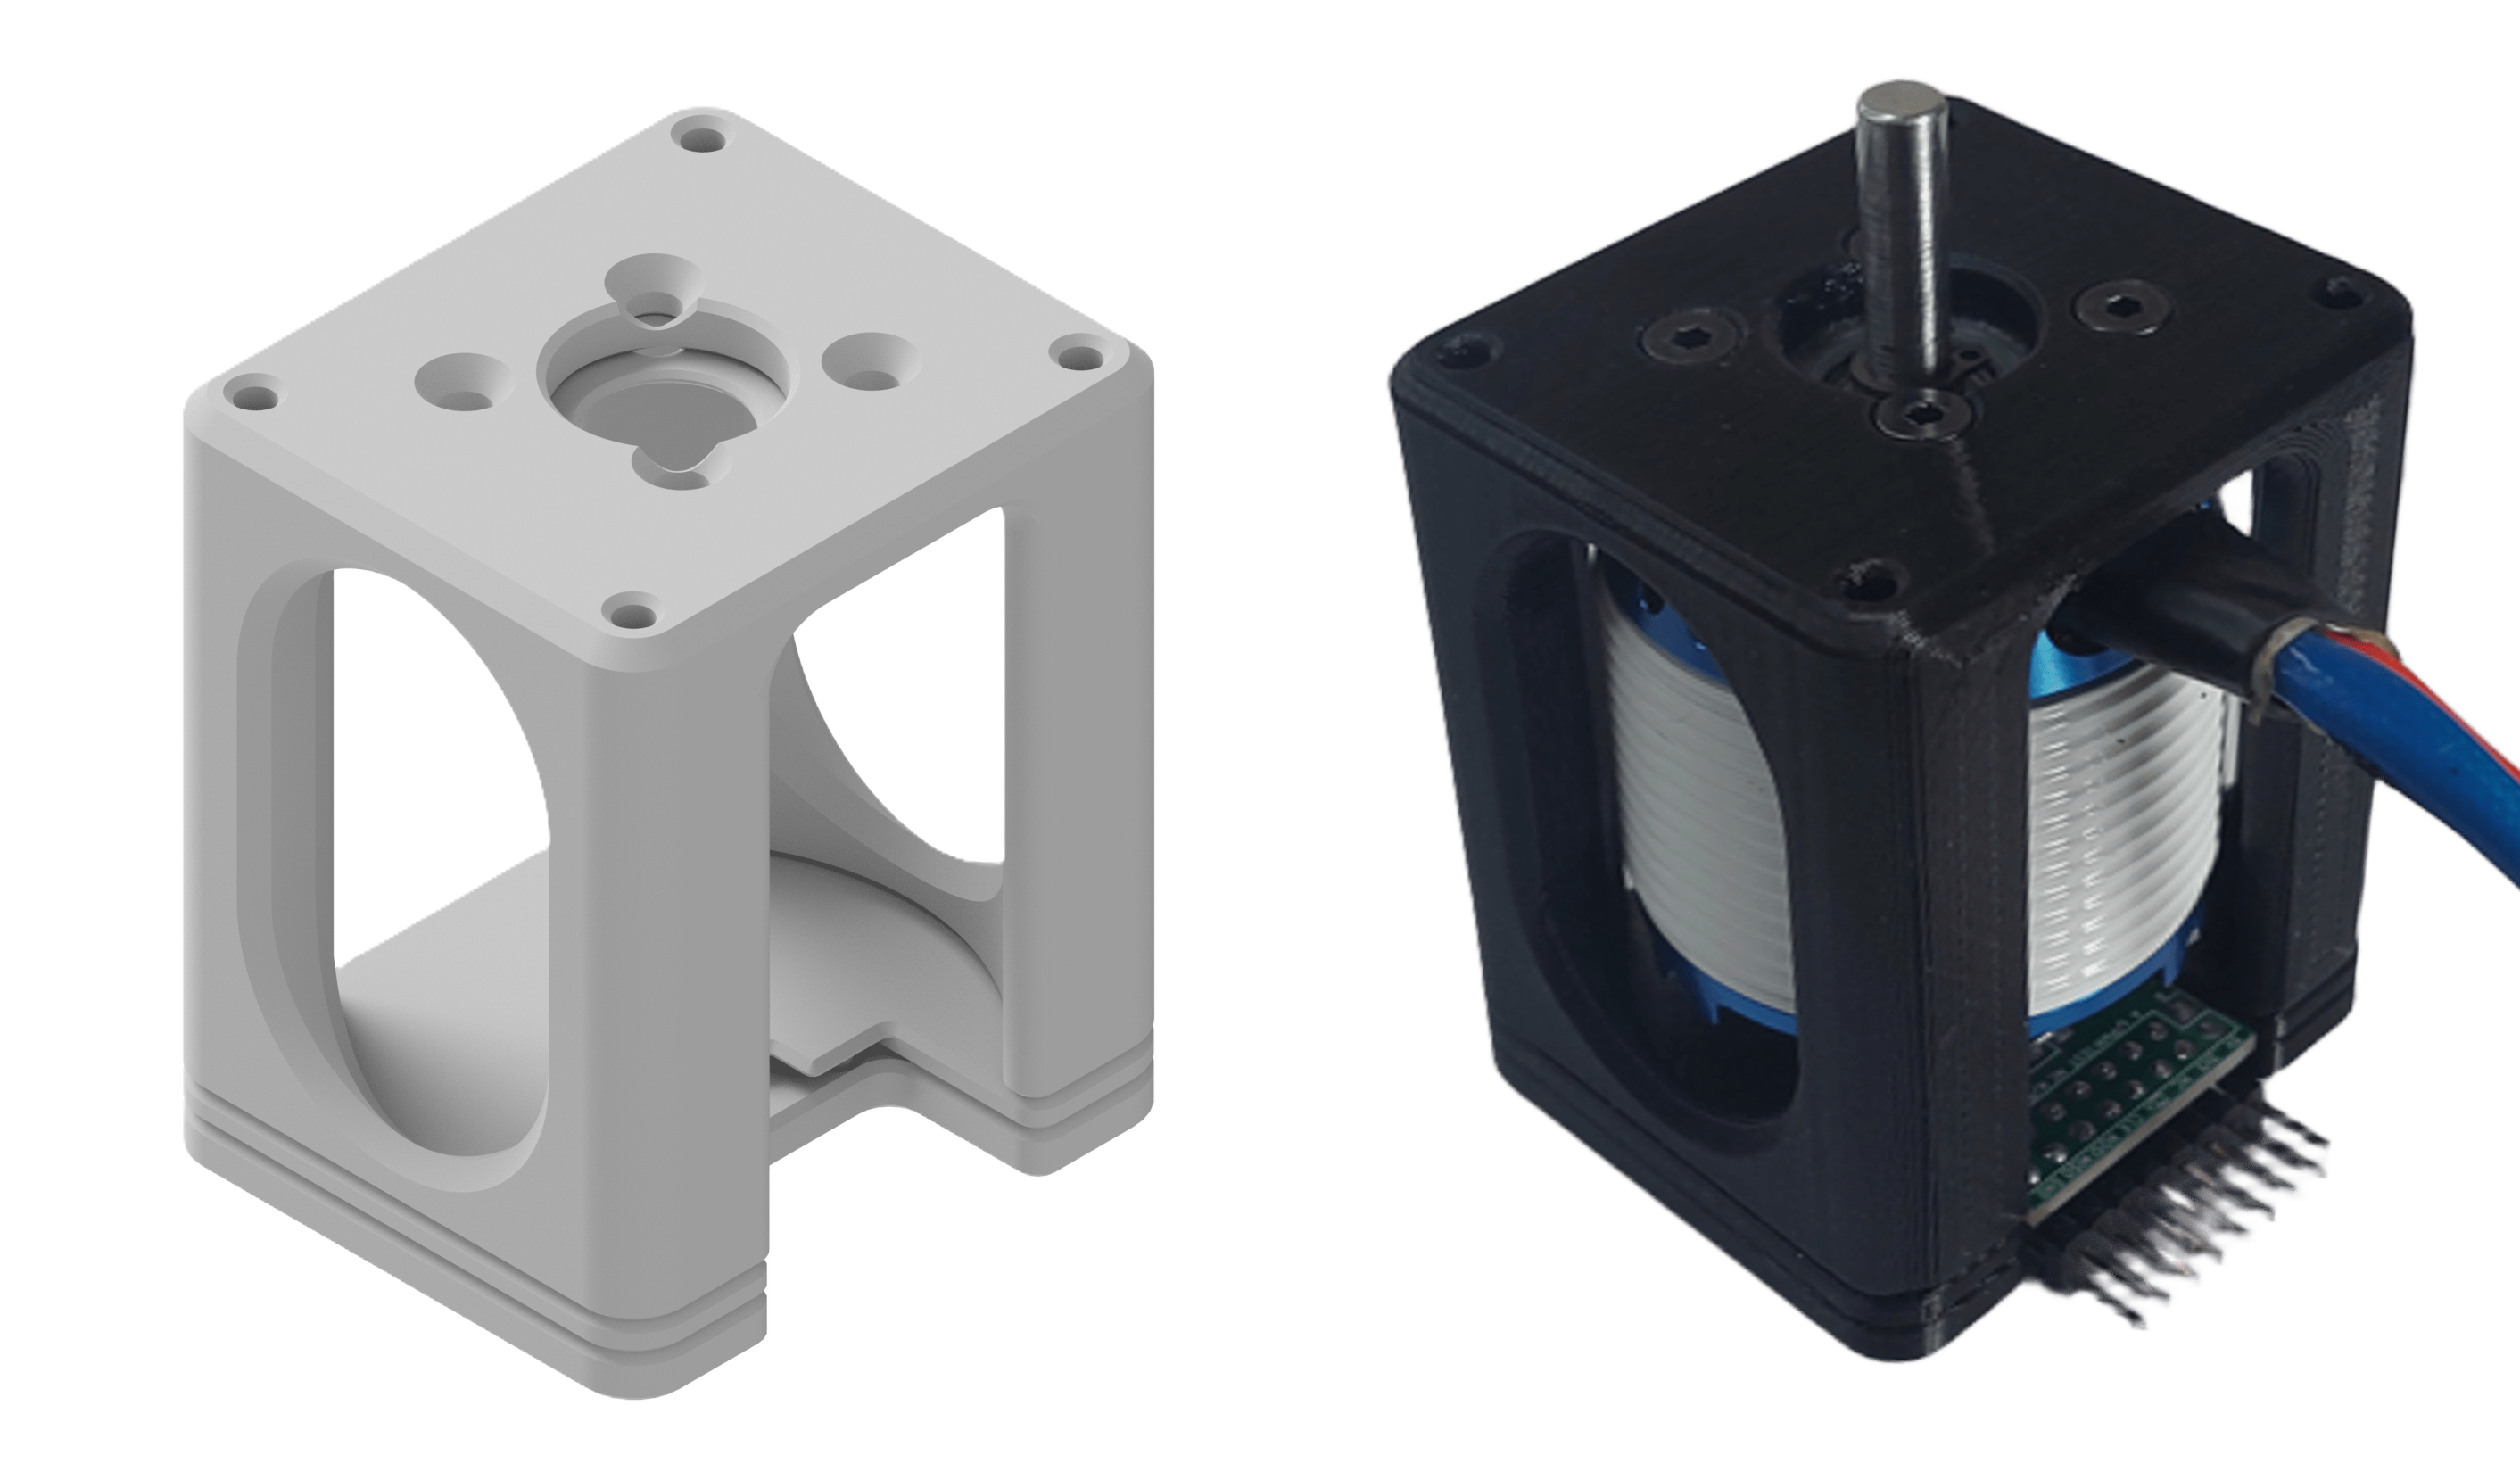
\includegraphics[width=0.5\textwidth]{imagenes/Motor/conjunto.png}
	\caption{Montura motor-encoder.}
	\label{fig:Montura}
\end{figure}
\FloatBarrier

\begin{figure}[ht]
	\centering
	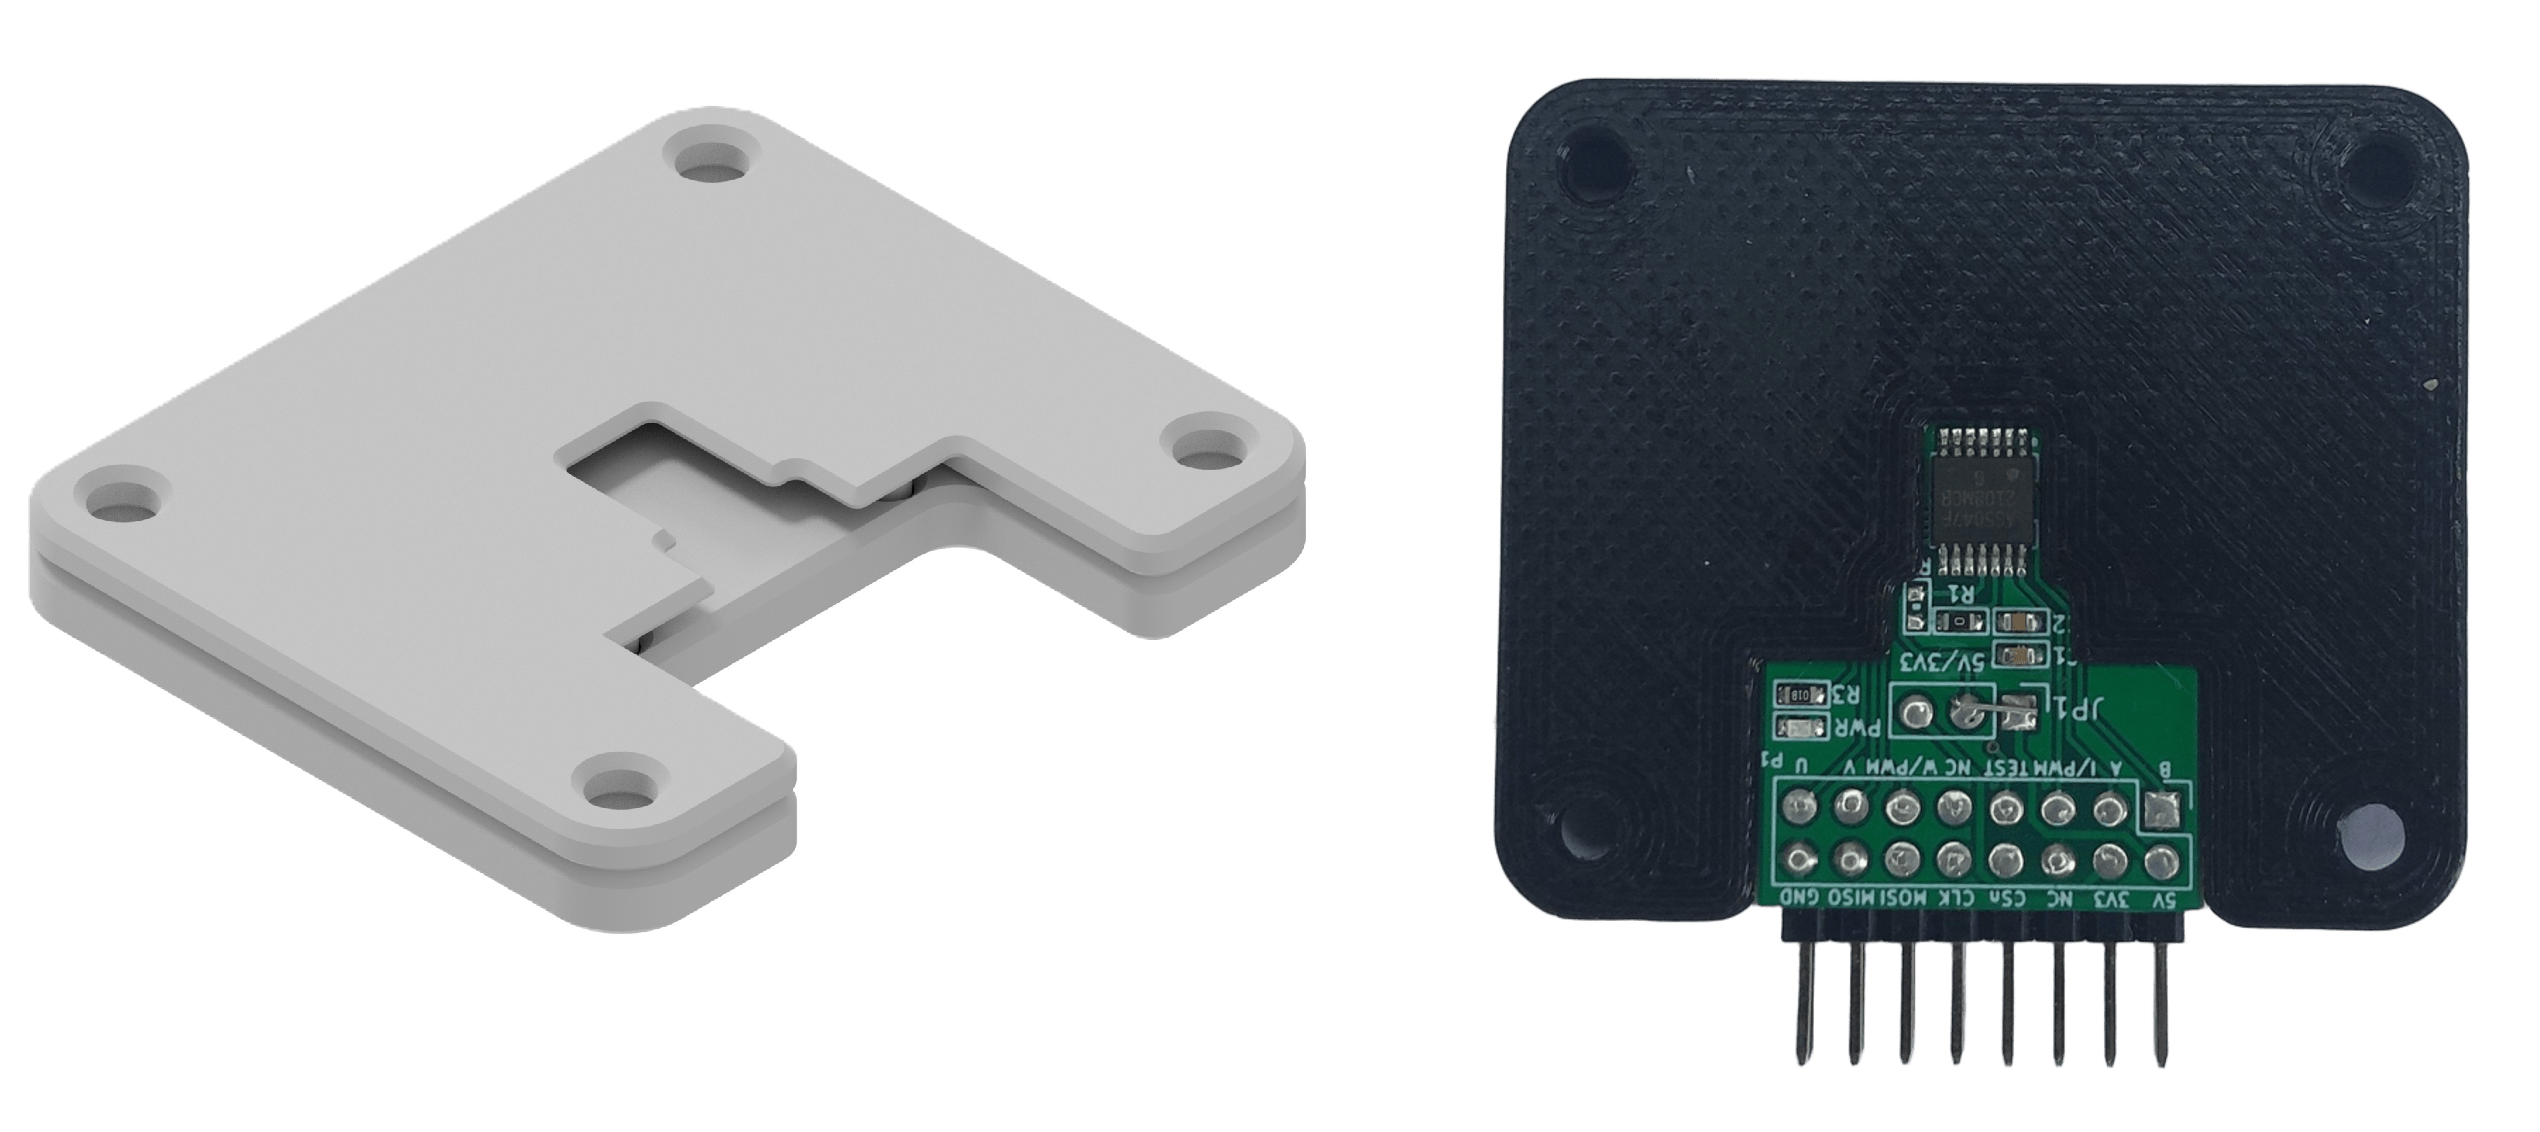
\includegraphics[width=0.5\textwidth]{imagenes/Motor/encoder.png}
	\caption{Socket Encoder.}
	\label{fig:encoder}
\end{figure}
\FloatBarrier

También se diseñó un socket con el fin de mantener el imán necesario para el funcionamiento del en coder en el centro del eje del motor.

\begin{figure}[ht]
	\centering
	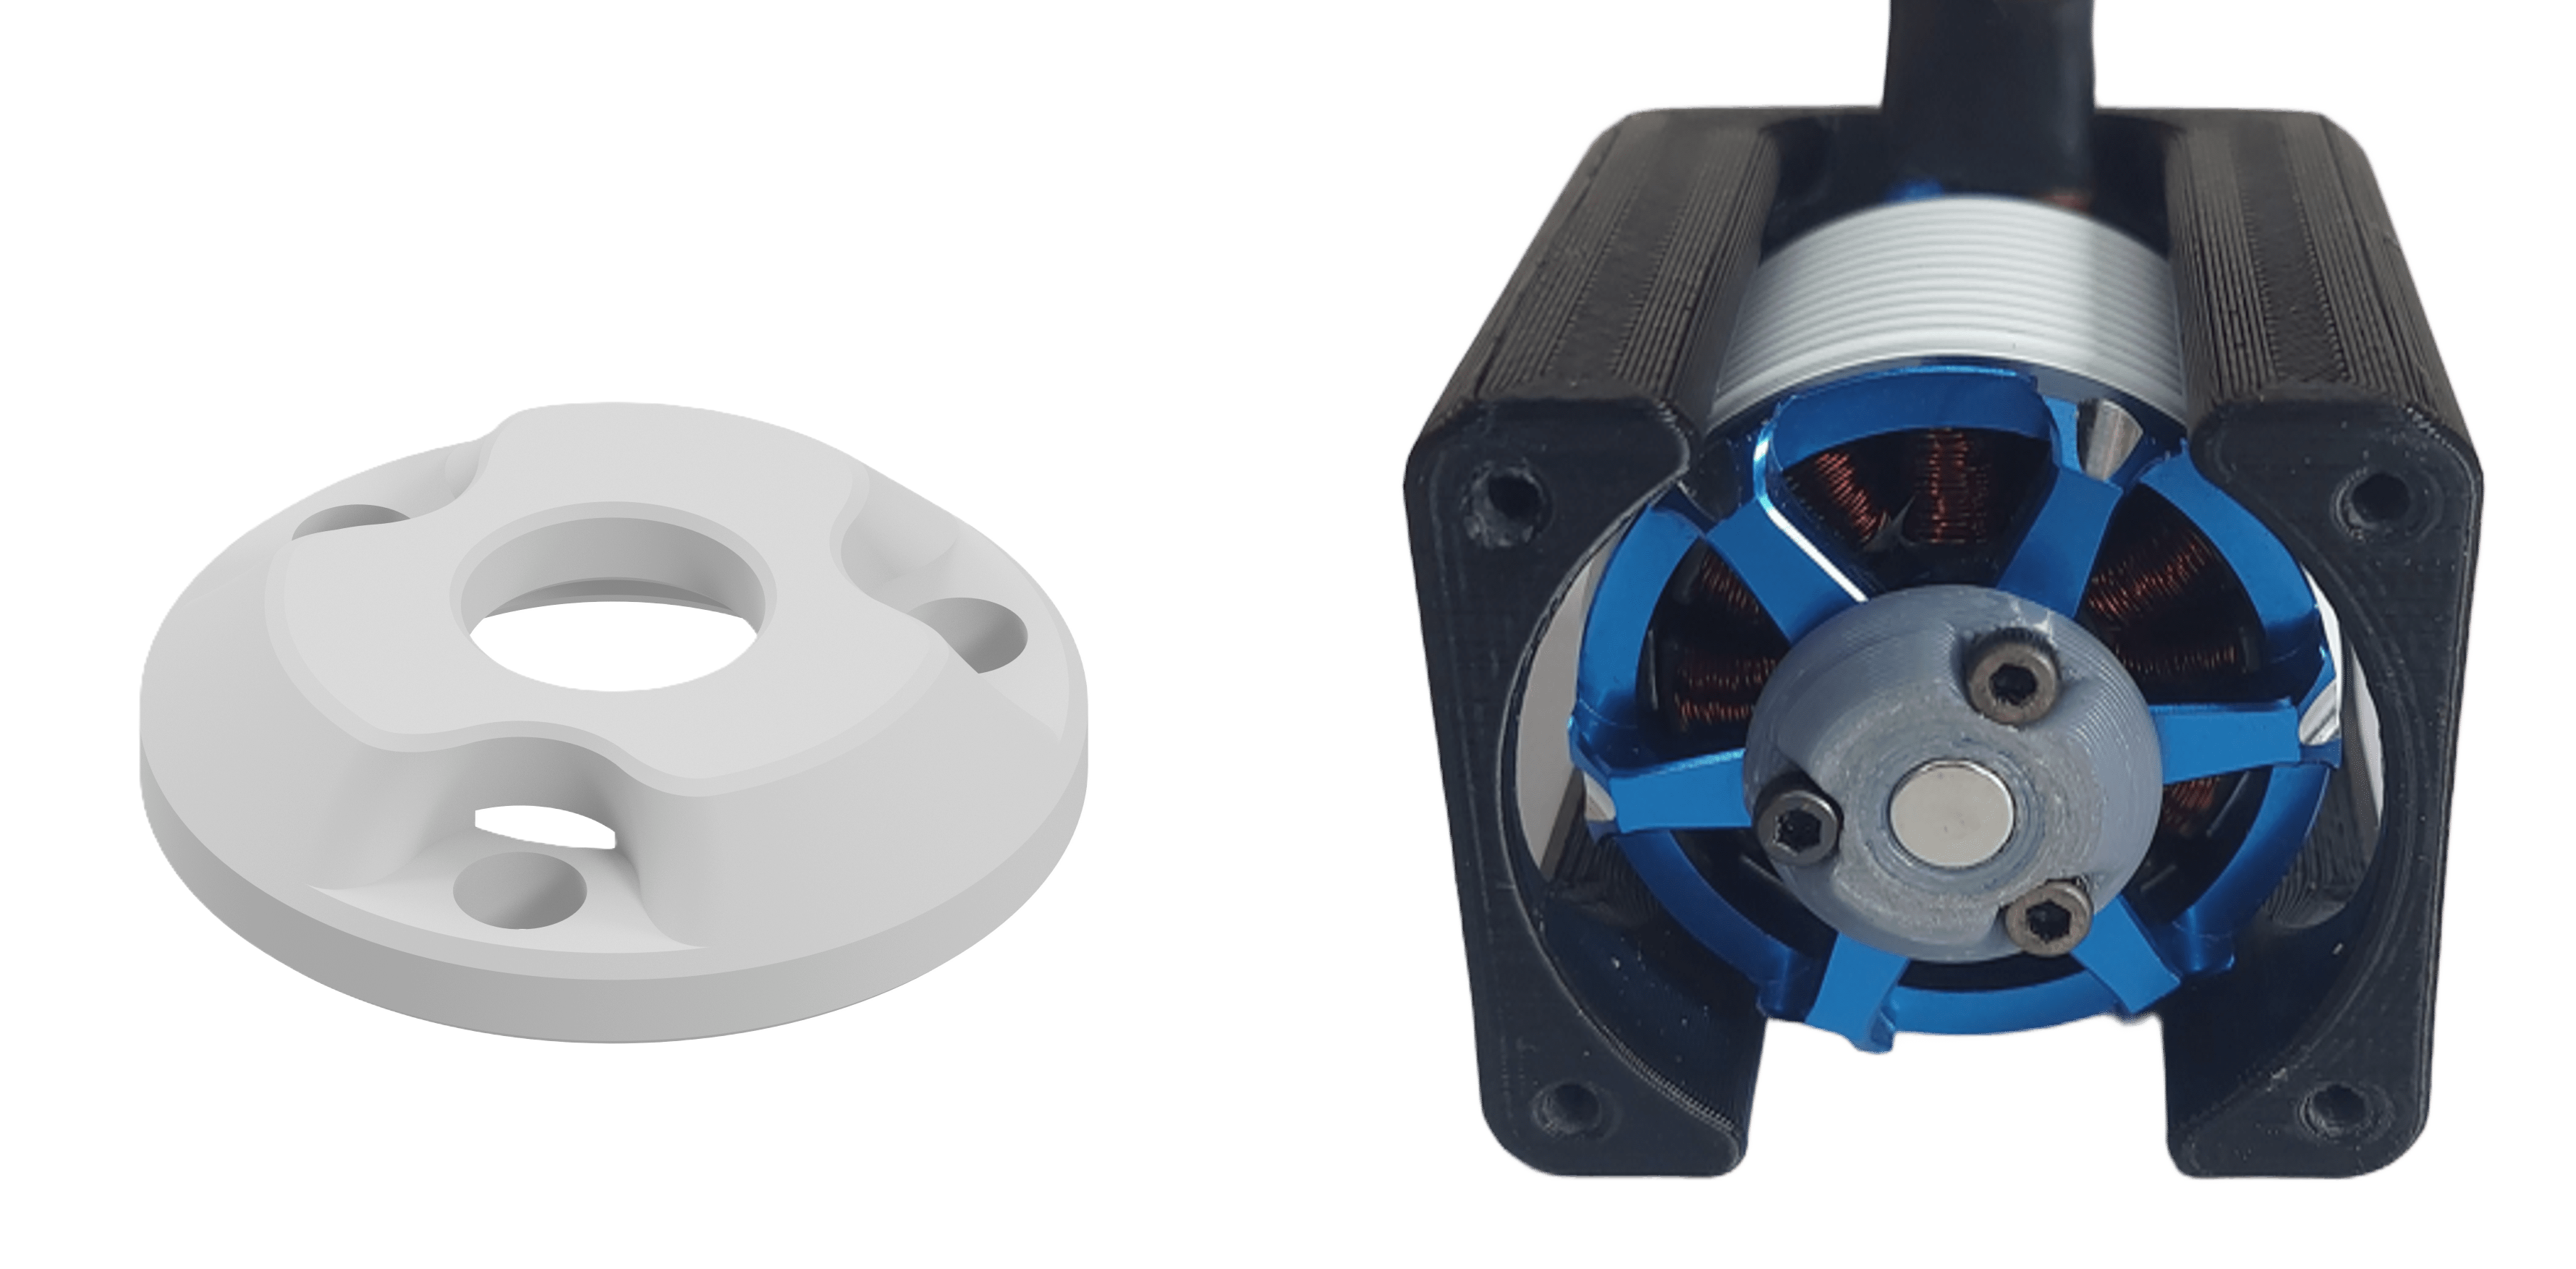
\includegraphics[width=0.5\textwidth]{imagenes/Motor/iman.png}
	\caption{Socket imán axial.}
	\label{fig:iman}
\end{figure}
\FloatBarrier

\newpage
\subsection{Puente Mosfet}

El puente mosfet es una de las partes del hardware mas critica, este se encarga de realizar las conmutaciones en las fases del motor, se divide en 3 piernas (o fases) iguales, donde cada pierna está conformada por 2 mosfets de tipo N en configuración push-pull, es decir, se tiene un mosfet alto conectado a $V+$ y un mosfet bajo conectado a $V-$. cada mosfet tiene su propia señal de gate las cuales se deben controlar de forma adecuada para evitar cortocircuitos. es importante considerar que cada pierna del puente debe soportar por lo menos la corriente máxima del motor, aun que idealmente se deja un margen de seguridad de 2 a 3 veces la corriente máxima, considerando la corriente de 65A del sunnysky X3120, los mosfets deberán de soporta al menos 195A continuos y un voltaje Drain-source sobre los 25.2V para poder trabajar con la batería 6S.

\begin{figure}[ht]
	\centering
	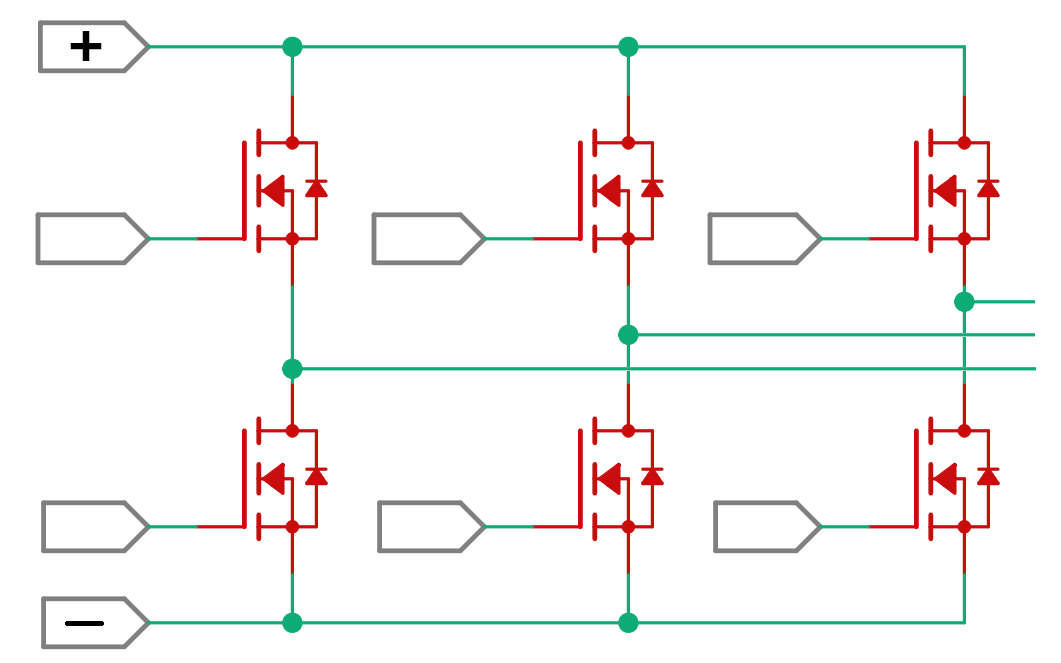
\includegraphics[width=0.8\textwidth]{imagenes/Diagramas/puente mosfet.png}
	\caption{Esquema puente MOSFET.}
	\label{puente_MOSFET}
\end{figure}
\FloatBarrier

Se utilizó el mosfet \textbf{BSC011N03LSI} de la marca Infineon, es un Mosfet de tipo N con un voltaje Drain-source de 30V, estos mosfets soportan una corriente continua de 100A.

\begin{table}[h!]
	\centering
	\caption{Características del MOSFET BSC011N03LSI.}
	\begin{tabular}{l l c c c l}
		\hline
		\textbf{Parámetro}            & \textbf{Variable} & \textbf{Min} & \textbf{Typ} & \textbf{Max} & \textbf{Unidad}    \\
		\hline
		Tensión de drenaje-fuente     & $V_{DS}$          &              &              & 30           & $\mathrm{V}$       \\
		Resistencia encendido         & $R_{DS(on)}$      & 0.9          & 1.1          & 1.5          & $\mathrm{m\Omega}$ \\
		Corriente continua de drenaje & $I_D$             &              &              & 100          & $\mathrm{A}$       \\
		Corriente de pulso drenaje    & $I_{D,pulse}$     &              &              & 400          & $\mathrm{A}$       \\
		Tensión umbral del gate       & $V_{GS(th)}$      & 1.2          &              & 2            & $\mathrm{V}$       \\
		Carga de puerta total         & $Q_g$             &              & 34           & 45           & $\mathrm{nC}$      \\
		Potencia de disipación        & $P_{tot}$         &              &              & 96           & $\mathrm{W}$       \\
		\hline
	\end{tabular}
\end{table}
\FloatBarrier

\newpage
\subsection{Controladores de Puerta}

El controlador de puerta (gate driver) se encarga de recibir las señales PWM provenientes del microcontrolador ,y en consecuencia, activar o desactivar los MOSFETs en cada pierna del puente. Su función principal es proporcionar la corriente y el voltaje adecuados para encender y apagar rápidamente los MOSFETs, garantizando una conmutación eficiente y minimizando las pérdidas de energía.

\begin{figure}[ht]
	\centering
	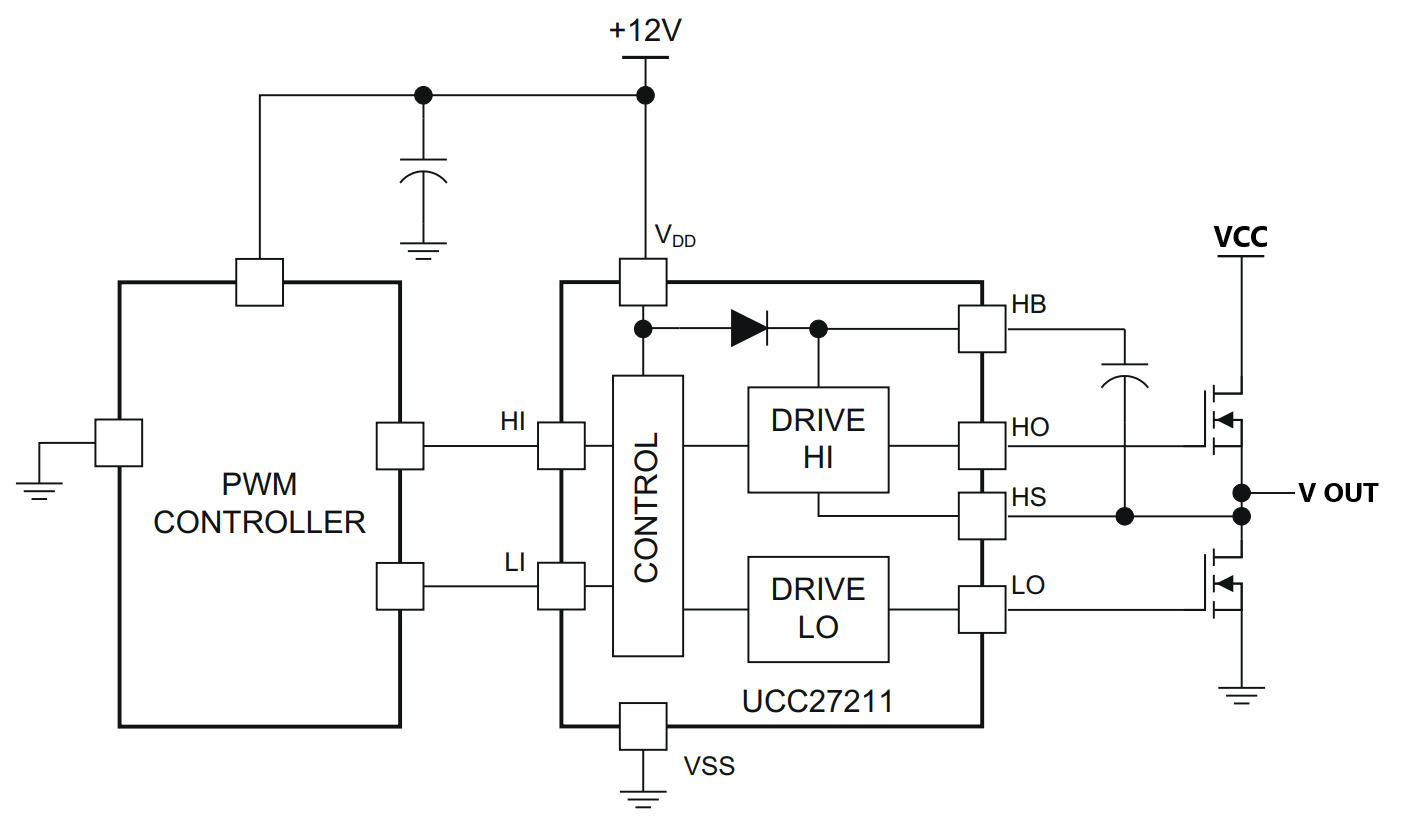
\includegraphics[width=0.8\textwidth]{imagenes/Diagramas/UCC27211.png}
	\caption{Esquema UCC27211.}
	\label{UCC27211}
\end{figure}
\FloatBarrier

Se utilizó el controlador de puerta \textbf{UCC27211} de Texas Instruments, el cual es un driver de doble canal diseñado específicamente para controlar pares de MOSFETs. Este dispositivo ofrece entradas de control independientes para los MOSFETs de alta (\texttt{H In}) y baja (\texttt{L In}), lo que permite un control preciso y flexible de cada transistor de potencia.

\begin{table}[ht]
	\centering
	\caption{Tabla de Lógica del UCC27211}
	\label{tab:device_logic}
	\begin{tabular}{|c|c|c|c|c|}
		\hline
		\textbf{H In} & \textbf{L In} & \textbf{H Out} & \textbf{L Out} & \textbf{V Out} \\ \hline
		L             & L             & L              & L              & Z              \\ \hline
		L             & H             & L              & H              & GND            \\ \hline
		H             & L             & H              & L              & VCC            \\ \hline
		H             & H             & H              & H              & Corto          \\ \hline
	\end{tabular}
\end{table}
\FloatBarrier

\newpage
Es importante destacar que el UCC2711 no incorpora protección interna contra la conducción simultánea de ambos MOSFETs conocido como \textbf{shoot-through}. Este fenómeno ocurre ambos MOSFETs de una pierna conducen al mismo tiempo, generando un cortocircuito entre el suministro de voltaje y tierra. Para evitar esta situación es importante agregar un tiempo entre la conmutación de las señales de entrada conocido como \textbf{Dead-Time}, el cual se estima considerando los tiempos de conmutación del controlador de puerta junto al tiempo de conmutación del mosfet

\begin{figure}[ht]
	\centering
	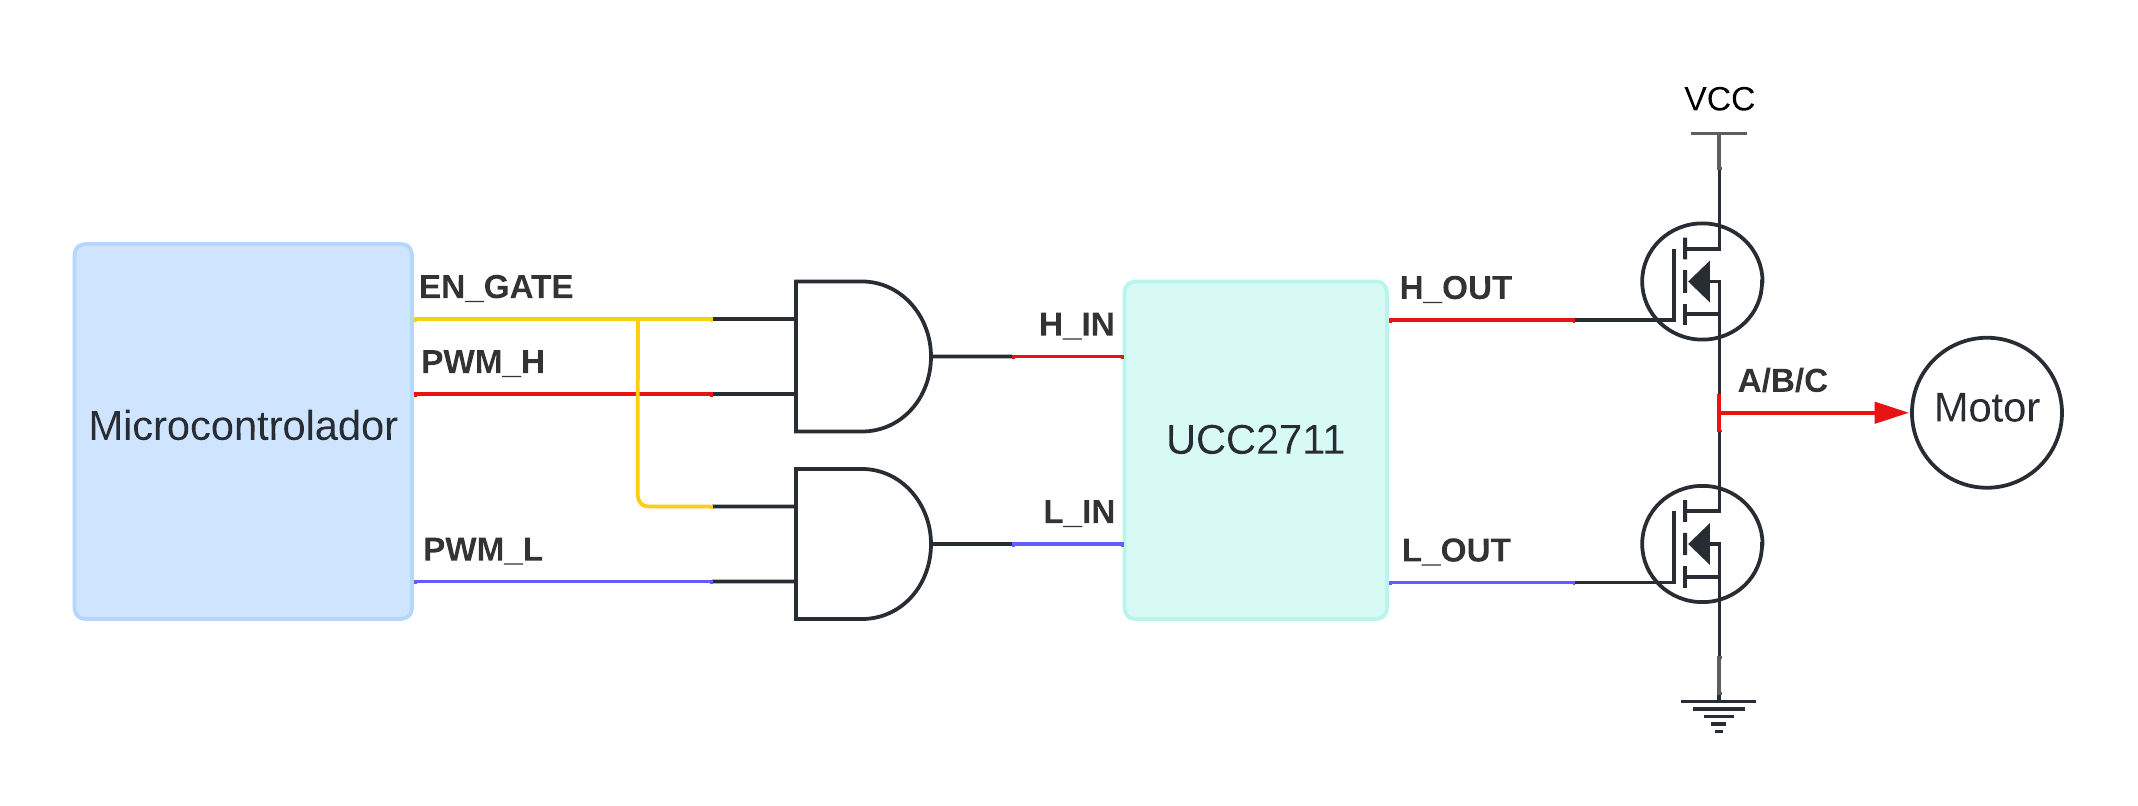
\includegraphics[width=0.8\textwidth]{imagenes/Diagramas/Diagramas - AND.png}
	\caption{Esquema de control PWM con las compuertas AND.}
	\label{fig:control-pwm-and}
\end{figure}
\FloatBarrier

El UCC27211 no dispone de un pin para activar o desactivar el control de los mosfets, por su parte, la única forma de desactivar el puente mosfet en su totalidad es llevar las señales de entrada alta (H In) y baja (L In) a un estado bajo (L), además el microcontrolador al realizar esta acción puede llegar a perder el control sobre el estado de las señales PWM y asi generar por un breve momento un estado de doble activación de los mosfet. para evitar esto se agregaron externamente comportas AND modelo SN74LVC1G08DBVR en cada señal PWM, con el fin de poder cortar las señales desde el microcontrolador de forma segura.

\begin{table}[ht]
	\centering
	\caption{Tabla de Lógica del UCC27211 con AND}
	\label{UCC27211_logic}
	\begin{tabular}{|c|c|c|c|c|c|c|c|}
		\hline
		\textbf{EN GATE} & \textbf{PWM H} & \textbf{PWM L} & \textbf{H In} & \textbf{L In} & \textbf{H Out} & \textbf{L Out} & \textbf{V Out} \\
		\hline
		H                & L              & L              & L             & L             & L              & L              & Z              \\ \hline
		H                & L              & H              & L             & H             & L              & H              & GND            \\ \hline
		H                & H              & L              & H             & L             & H              & L              & VCC            \\ \hline
		H                & H              & H              & H             & H             & H              & H              & Corto          \\ \hline
		L                & X              & X              & L             & L             & L              & L              & Z              \\ \hline
	\end{tabular}
\end{table}
\FloatBarrier


\newpage
\subsection{Sensores de Corriente}

Para el sensor de corriente se opto por una configuración de resistencia shunt en la salida del puente mosfet como se puede ver en la figura \ref{INA240}, esta configuración aprovecha la caída de tension provocada por la resistencia de valor conocido para poder calcular la corriente del circuito, se utiliza un amplificador instrumental especializado en esta aplicación, en este caso se utilizó el INA240A1 que tiene una ganancia de 20V/V y se le aplica un offset equivalente a la mitad voltaje de referencia de 3.3V.

\begin{figure}[ht]
	\centering
	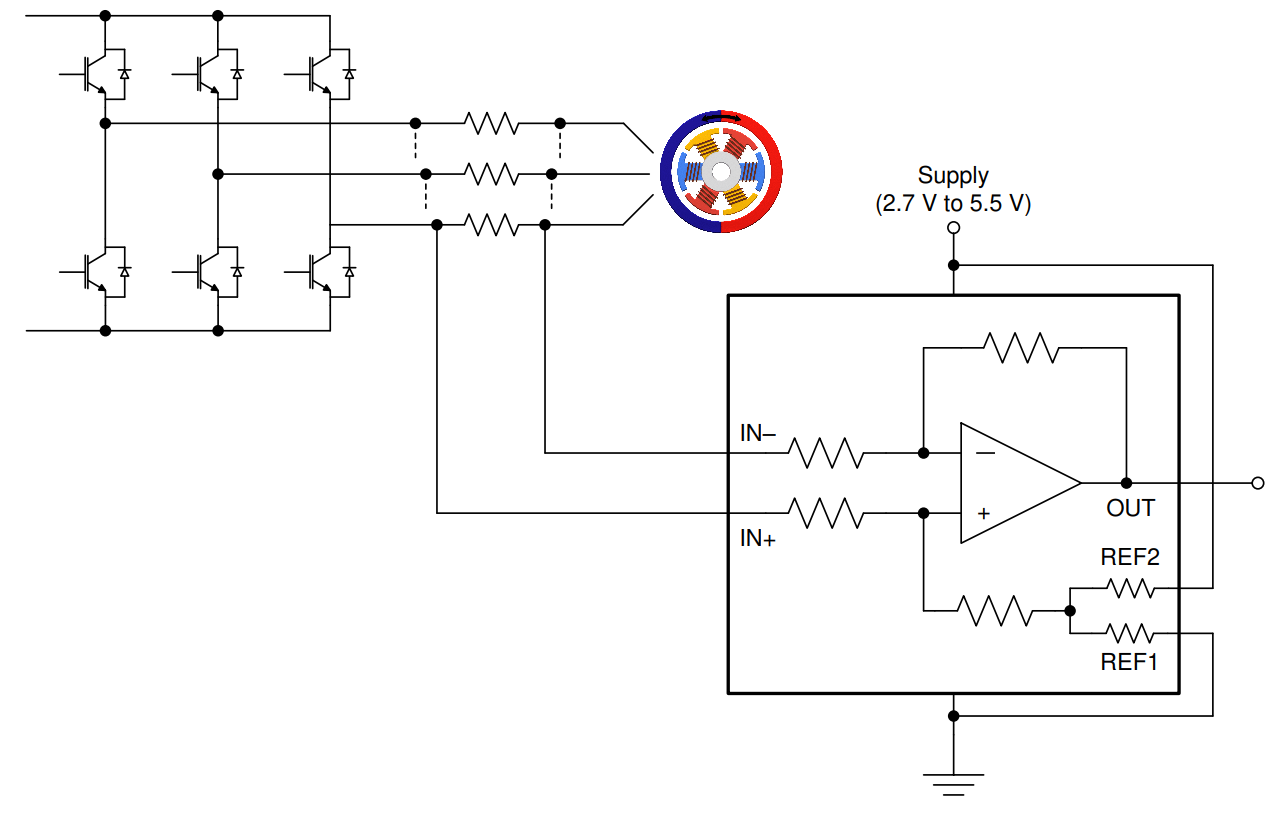
\includegraphics[width=0.6\textwidth]{imagenes/Diagramas/INA240.png}
	\caption{Esquema INA240.}
	\label{INA240}
\end{figure}
\FloatBarrier

Para la resistencia shunt se utilizó una doble resistencia en paralelo como se ve en la figura \ref{PCB_pierna_C}, la resistencia es de 1m$\Omega$ y 5W de disipación lo que da una una resistencia equivalente de 500$\mu\Omega$ y 10W de disipación, para determinar la corriente máxima que puede pasar la resistencia conociendo su valor en ohmios \( R \) y la potencia \( P \) en vatios, se puede calcular utilizando la siguiente fórmula:

\[
	I_{\text{max}} = \sqrt{\frac{P}{R}}
\]

Donde:
\begin{itemize}
	\item \( I_{\text{max}} \) es la corriente máxima,
	\item \( P \) es la potencia en vatios (W),
	\item \( R \) es el valor de la resistencia en ohmios ($\Omega$).
\end{itemize}

De esta forma se determina que el máximo de corriente continua que puede circular por las resistencias es de 141.42A.

\newpage
\section{Implementación del puente MOSFET}
El diseñó de la PCB esta realizado en el software de Eagle, ya que este software de diseñó contiene un entorno amigable para el diseñó de  PCBs, además de tener una gran adaptabilidad según el tipo de proyecto a realizar.

\begin{figure}[ht]
	\centering
	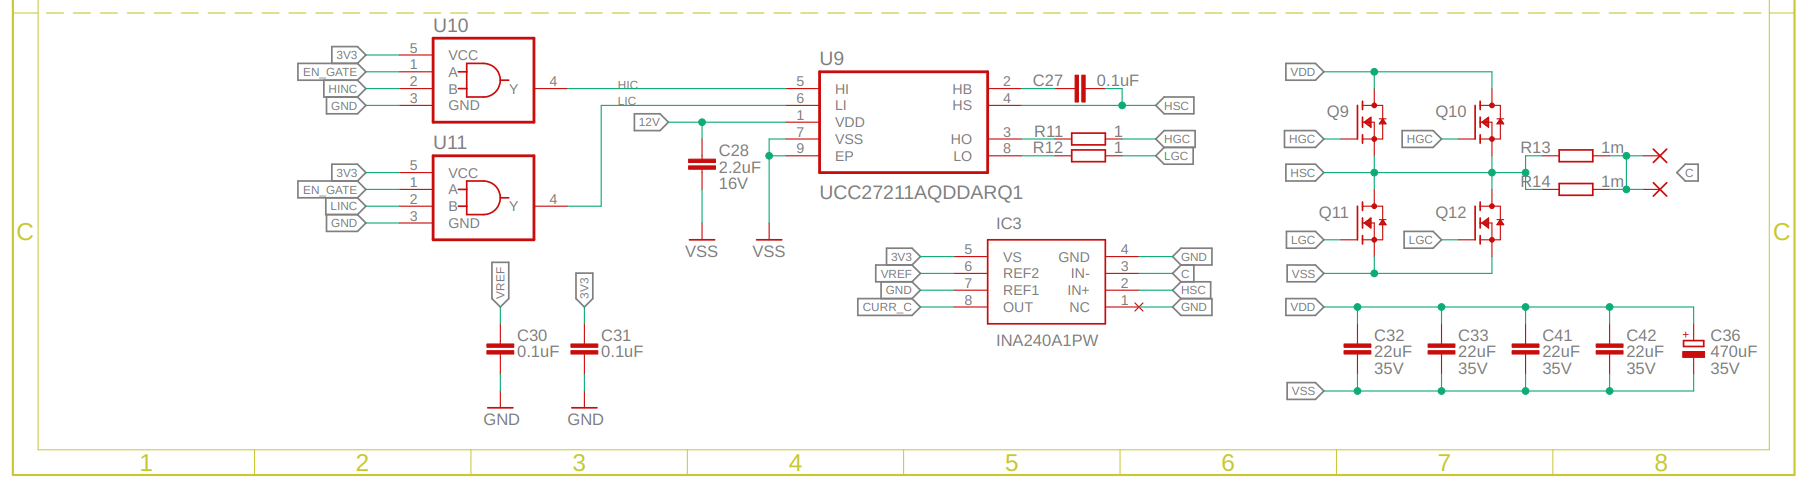
\includegraphics[width=0.9\textwidth]{imagenes/Diagramas/esquematico_pierna_C.png}
	\caption{Esquemático de la pierna C del inversor.}
	\label{esquema_pierna_C}
\end{figure}
\FloatBarrier

Se conectaron condensadores de desacoplo de 100$\text{nF}$ en las entradas de alimentación de los diferentes componentes para eliminar ruido provenientes de los reguladores de voltaje. además se agrego un regulador de voltaje de referencia de 3.3V el cual sirve de referencia para los ADC y además se utiliza para el ajuste del offset en los amplificadores INA240.

\begin{figure}[ht]
	\centering
	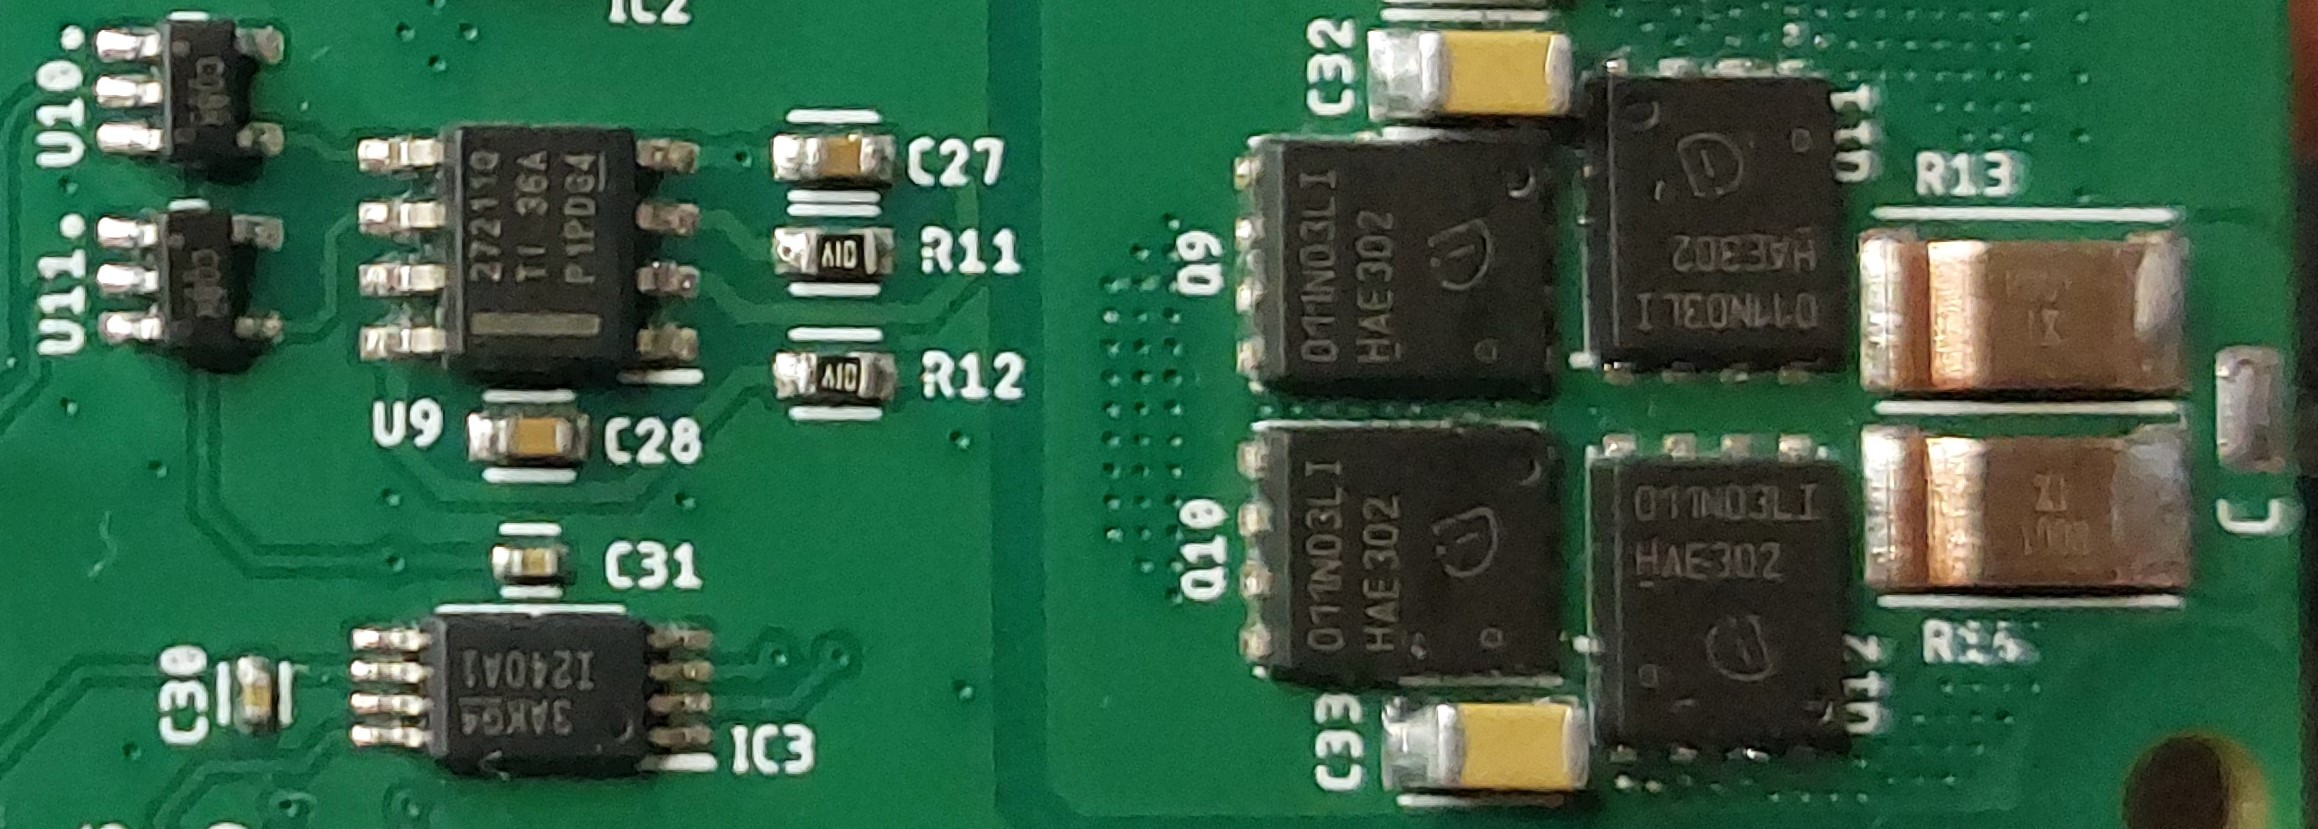
\includegraphics[width=0.8\textwidth]{imagenes/PCB/FULL_Pierna_C.jpg}
	\caption{Pierna C del inversor.}
	\label{PCB_pierna_C}
\end{figure}
\FloatBarrier

Basado en las características del mosfet el cual soporta una corriente continua de 100 A, utilizar 2 mosfet por pierna seria insuficiente, por lo que se opto por utilizar configuración de 4 mosfets con doble mosfet en paralelo, de esta forma se puede considerar una capacidad total de 200A continuos, despreciando las leves diferencias entre los mosfets del mismo modelo.

\begin{figure}[ht]
	\centering
	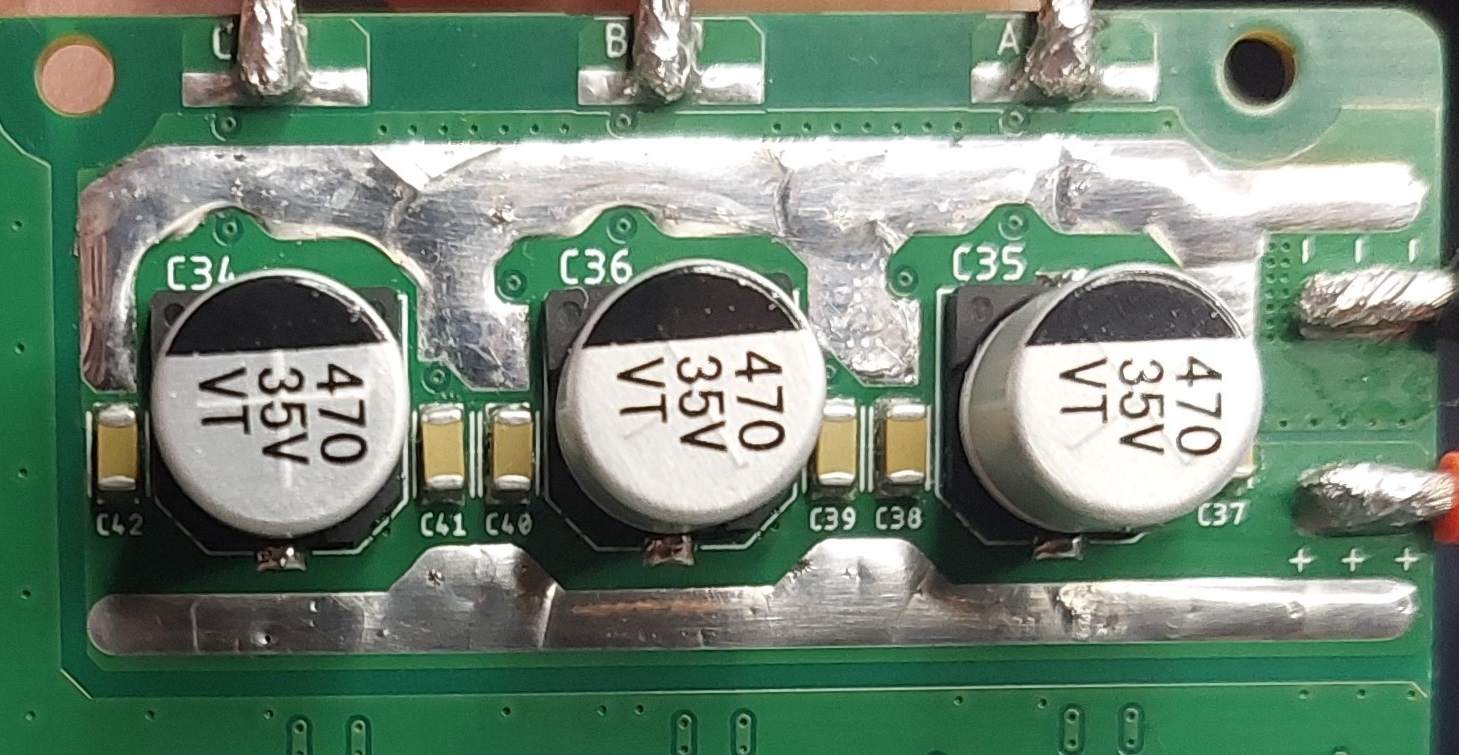
\includegraphics[width=0.8\textwidth]{imagenes/PCB/alimentacion mosfet.jpg}
	\caption{alimentación del Puente MOSFET.}
	\label{alimentacion}
\end{figure}
\FloatBarrier

En el reverso de la \href{https://www.youtube.com/watch?v=J---aiyznGQ}{PCB} se realizó un estañado de las pistas de alimentación de alta corriente correspondientes al puente mosfet, en respuesta a las altas exigencias demandadas por el motor. A la vez que se dispusieron varios capacitores electrolíticos de 470$\mu\text{F}$ y capacitores cerámicos de 22$\mu\text{F}$ estratégicamente posicionados para mitigar los picos de corriente y garantizar la estabilidad del sistema.

La PCB fue fabricada a pedido por JLCPCB debido a su plataforma intuitiva, lo cual simplifica significativamente el proceso de producción. Además, el diseñó de la PCB consta de 6 capas, y JLCPCB ofrece costos más competitivos para este tipo de configuraciones multicapa, lo que lo convierte en una opción económica y eficiente.

\newpage
\section{Observaciones y posibles mejoras}

Respecto al motor, se constató que presenta un elevado efecto de \emph{cogging torque}, lo cual incide de manera significativa en la estabilidad de la velocidad de giro. Existen sistemas comerciales que permiten calibrar y compensar este fenómeno. Sin embargo, en el presente proyecto no se incluyó dicha funcionalidad. Además, al someter el motor a cargas elevadas, se observó un notable incremento de temperatura, pudiendo alcanzar valores superiores al punto de deformación del material PLA utilizado en la fabricación del soporte para el \emph{encoder}. En consecuencia, se recomienda emplear materiales más resistentes al calor, como PETG o ABS, para la elaboración de este soporte.

En cuanto al puente MOSFET, el principal inconveniente radica en la activación simultánea de los transistores (conocida como “doble activación”), cuya causa podría ser una estimación inadecuada del \emph{deadtime} o posibles errores en las señales de control. Para mitigar este problema, se sugiere incorporar compuertas lógicas adicionales que eviten la conducción simultánea o, alternativamente, utilizar controladores de puerta con protecciones integradas, como el ISL6208 de Renesas, el cual ofrece protección activa contra la doble activación y elimina la necesidad de insertar un \emph{deadtime}. No obstante, es importante considerar que dicho controlador soporta menores voltajes de bus para los MOSFET.

Por último, se detectó que, en condiciones de carga extrema, las caídas de tensión en las pistas de alimentación de la PCB alcanzan niveles considerables, incluso cuando se aplica estañado. Para resolver esta situación, se recomienda aumentar el ancho de las pistas o soldar barras de cobre, con el fin de reducir su resistencia y mejorar la distribución de la corriente.

\newpage
\chapter{Firmware}
\section{Introducción}
Este capítulo busca documentar el desarrollo e implementación del firmware, partiendo por la revisión de los periféricos utilizados y la configuración de estos, finalmente se revisar a grandes rasgos el diseñó e implementación del algoritmo para el control FOC.

\section{Microcontrolador y periféricos}
Se utilizó un microcontrolador de la serie H7 de STM32, esta es la serie de alto performance de STM32 que incorpora un núcleo ARM Cortex M7 con unidad de calculo para punto flotante de doble precision (FPU). el modelo especifico es STM32H743VIT6, su núcleo trabaja a 480MHz, tiene de 1MB de memoria RAM y 2MB de memoria flash, donde asi una potencia de computo y capacidad bastante elevada para un microcontrolador.

\begin{itemize}
	\item \textbf{Core}: Arm Cortex-M7 de 32bits a 480 MHz, FPU de doble precisión.
	\item \textbf{Memoria Flash}: 2 MB.
	\item \textbf{RAM}: 1 MB total (192 KB de RAM DTCM, 864 KB de SRAM).
	\item \textbf{Voltaje de operación}: 1.62 V - 3.6 V.
	\item \textbf{Empaquetado}: LQFP-100 (14 x 14 mm).
	\item \textbf{Entradas/Salidas}: 82 I/O.
	\item \textbf{Periféricos de comunicación}: USART, UART, SPI, CAN FD, USB, Ethernet.
	\item \textbf{Timers}: Hasta 22 timers (PWM, encoder, control de motores, etc.).
	\item \textbf{ADC}: 3x ADC tipo SAR de 16 bits (hasta 3.6 MSPS).
	\item \textbf{Programación y Depuración}: Interfaz SWD y JTAG.
\end{itemize}

Los periféricos en un microcontrolador son piezas de hardware especializados en una función que van integrados en el microcontrolador y permiten interactuar con el mundo exterior a traves de sus señales eléctricas, ya sean entradas o salidas, digitales o análogas. en el ecosistema de STM32 existe la herramienta \textbf{STM32CubeMX} que permite configurar todos los periféricos del microcontrolador desde una interfaz gráficas fácil de entender para posteriormente poder generar un código C que implemente todas las configuraciones en el microcontrolador utilizando las librerías HAL de STM32, de esta forma \textbf{STM32CubeMX} genera un código base desde el que empezar a programar el firmware con todos los periféricos ya configurados.

\subsection{Configuración de Timers}
Los timers en los microcontroladores STM32 permiten contar eventos y controlar pines de salida según dichos eventos. Estos eventos pueden provenir del reloj interno o de señales externas. La familia STM32 ofrece gran flexibilidad para configurar modos de conteo, fuentes de reloj y funcionalidades específicas, como la generación de PWM o la captura de entrada.

\subsubsection{Timer 1}
El Timer 1, al ser de tipo \textbf{Advanced-control} de hasta 16 bits, está especialmente diseñado para la generación de señales PWM con complementarias con inserción de \emph{dead time}, lo que facilita el control de puentes MOSFET. Se configura en modo \emph{center-aligned} (cuenta ascendente y descendente), permitiendo tener salidas PWM adecuadas para su uso con el SVM.

\begin{table}[h!]
	\centering
	\begin{tabular}{| l | l |}
		\hline
		\textbf{Parámetro en CubeMX}         & \textbf{Valor}           \\
		\hline
		Clock Source                         & Internal Clock (240 MHz) \\
		Counter Mode                         & Center Aligned mode 3    \\
		Counter Period (16 bits)             & 5000                     \\
		Trigger Event Selection TRGO         & Update Event             \\
		Dead Time                            & 50                       \\
		\hline
		Channel 1                            & PWM Generation CH1 CH1N  \\
		PWM Generation Channel 1 and 1N Mode & PWM mode 1               \\
		\hline
		Channel 2                            & PWM Generation CH2 CH2N  \\
		PWM Generation Channel 2 and 2N Mode & PWM mode 1               \\
		\hline
		Channel 3                            & PWM Generation CH3 CH3N  \\
		PWM Generation Channel 3 and 3N Mode & PWM mode 1               \\
		\hline
	\end{tabular}
	\caption{Configuración del Timer 1 en CubeMX.}
	\label{TIM1_config}
\end{table}
\FloatBarrier

Dado que el reloj base es de 240 MHz y el \texttt{Counter Period} se establece en 5000, se obtiene un evento de desborde a 48 kHz (\(\frac{240\text{ MHz}}{5000} = 48\text{ kHz}\)) (El desborde es cuando el contador llega a su valor mínimo o máximo). En modo \emph{center-aligned}, cada ciclo completo de PWM comprende una fase ascendente y otra descendente, por lo que el PWM resultante es de 24 kHz. Además, las interrupciones del Timer 1 se generan en cada suceso de desborde , por lo que se dispone de una rutina de interrupción a 48 kHz para efectuar los cálculos y actualizaciones del lazo de control.

\subsubsection{Timer 3}
El Timer 3 es un timer de uso general de 16 bits, esta configurado en \textbf{modo encoder}, que permite contar los pulsos de un \emph{encoder} incremental sin intervención directa del firmware. De este modo, el microcontrolador registra por hardware los cambios de las fases A y B, en modo de conteo por 4 (X4). Se configura un \emph{input filter} para evitar pulsos espurios debidos al ruido, y se asigna un \texttt{Counter Period} de 65535 (el máximo para 16 bits), aun que este valor al corresponder solo a unos pocos giros del motor, es necesario implementar una gestión del desborde del timer.

\subsubsection{Timer 2}
El Timer 2 es un timer de uso general de 32 bits, se utiliza para adquirir mediciones precisas de tiempo relacionadas con la operación del encoder y la sincronización global del sistema. En CubeMX, se configura con reloj interno (\emph{Internal Clock} de 240 MHz) y se opera en modo \emph{Up} con un \texttt{Counter Period} de 4294967295 (valor máximo de 32 bits). A continuación, se describen las conexiones de cada canal:

\begin{table}[h!]
	\centering
	\begin{tabular}{| l | l |}
		\hline
		\textbf{Parámetro en CubeMX} & \textbf{Valor}                 \\
		\hline
		Trigger Source               & ITR0 (Timer 1 Trigger Out)     \\
		Clock Source                 & Internal Clock (240 MHz)       \\
		Counter Mode                 & Up                             \\
		Counter Period (32 bits)     & 4294967295                     \\
		\hline
		Channel 1                    & Input Capture triggered by TRC \\
		\hline
		Channel 2                    & Input Capture direct mode      \\
		Polarity                     & Both Edges                     \\
		\hline
		Channel 3                    & Input Capture direct mode      \\
		Polarity                     & Rising Edge                    \\
		\hline
	\end{tabular}
	\caption{Configuración del Timer 2 en CubeMX.}
	\label{TIM2_config}
\end{table}
\FloatBarrier

\begin{itemize}
	\item \textbf{Canal 1 conectado al Trigger Out del Timer 1:} Sirve para registrar con exactitud el instante en que el Timer 1 genera un evento de disparo. También se utiliza para gestionar el desborde del Timer 2 vía software, aumentando el rango de medición de tiempo (al ser de 32 bits, por defecto podría tardar unos 17,9 segundos en desbordar).

	\item \textbf{Canal 2 conectado a la salida \emph{XOR} de las señales A y B del encoder:} Genera un flanco de subida o bajada en cada pulso del encoder, permitiendo medir, mediante \emph{Input Capture}, el tiempo exacto entre pulsos y así refinar el cálculo de velocidad. Este método aporta mayor exactitud de tiempo que limitarse únicamente al uso del periodo de las interrupciones.

	\item \textbf{Canal 3 conectado a la señal \emph{Index} del encoder:} Aunque no se usa actualmente para una función concreta, permite determinar con precisión el momento en que dicha señal es \href{https://www.youtube.com/watch?v=FavUpD_IjVY}{activada}, facilitando futuras expansiones en la detección de referencias de giro.
\end{itemize}


\subsection{Configuración de los ADC y su integración con Timers y DMA} En los microcontroladores STM32, los conversores análogo-digital (ADC) se encargan de transformar voltajes analógicos en valores digitales dentro de un rango específico. En la serie H7, cada ADC ofrece una resolución de 16 bits y puede operar en dos modos principales:

\begin{itemize}
	\item \textbf{Conversión regular:} Permite leer hasta 16 canales en una secuencia programable. Se puede combinar con el módulo DMA (Acceso Directo a Memoria) para transferir los valores de conversión directamente a la memoria RAM sin necesidad de intervención del procesador, optimizando así el rendimiento.
	\item \textbf{Conversión inyectada:} Interrumpe la conversión regular para realizar, de forma prioritaria, hasta 4 mediciones de canales configurables. Este modo resulta útil cuando se requiere sincronizar lecturas en instantes precisos o realizar mediciones críticas con mínima latencia.
\end{itemize}

\textbf{DMA (Acceso Directo a Memoria):} El DMA es un módulo que permite trasladar datos entre periféricos y la memoria sin intervención de la CPU. De esta manera, mientras el ADC realiza sus mediciones, el DMA copia automáticamente los resultados a la RAM, liberando al núcleo del microcontrolador de dichas tareas y mejorando la eficiencia general del sistema.

\textbf{ADC 1:} El ADC 1 se encarga de la medición de las corrientes de fase, provenientes de los amplificadores operacionales que acondicionan las resistencias \emph{shunt}. Para sincronizar estas mediciones con las interrupciones del sistema  para que las lecturas estén disponibles a tiempo, se utiliza el \textbf{modo inyectado} del ADC, asociado a un disparo (\emph{trigger}) generado por el Timer 15.

\textbf{Timer 15:} El Timer 15 está configurado como esclavo del Timer 1 y emplea su \emph{Channel 1} en modo de comparación, sin generar salida directa pero conectado al (\emph{trigger out}), de esta forma se produce un pulso de sincronización con un pequeño desfase respecto a cuando se ejecute la interrupción del Timer 1. Este pulso activa la lectura inyectada en el ADC 1. De esta forma los resultados de las mediciones están listos en los registros del ADC cuando se ejecuta la rutina de interrupción.

\textbf{ADC 3:} El ADC 3 se utiliza para monitorear el voltaje de bus (por ejemplo, el suministro proveniente de la batería o la fuente principal). Dado que esta lectura no requiere una sincronización tan estricta, se configura en \textbf{modo regular}, habilitando conversiones continuas. Adicionalmente, se activa el módulo DMA para transferir los resultados al área de memoria en RAM, evitando sobrecargar la CPU con lecturas repetitivas.

\textbf{ADC 2:} Por último, el ADC 2 está destinado a la lectura de señales análogas utilizadas, en este caso, conectados a potenciómetros utilizados para el control de los setpoints en los controladores. Al igual que en el ADC 3, se configura en \textbf{modo regular} con conversiones continuas, y se emplea el DMA para automatizar la transferencia de los datos a memoria. Con esta configuración, se pueden atender varios canales análogos (por ejemplo, múltiples potenciómetros) sin que el procesador se vea afectado por interrupciones frecuentes.

\section{Estructura del Firmware}

Al utilizar la \href{https://www.youtube.com/watch?v=poa_QBvtIBA}{interrupción} del \textbf{Timer 1}, se genera un \emph{“doble hilo de ejecución”}: por un lado, la ejecución del programa en la función \texttt{int main()}, y por otro, la ejecución de la rutina de interrupción. Estos dos flujos deben interactuar entre sí sin interferir en el desempeño mutuo, lo cual exige un manejo adecuado de la \emph{sincronización} de las variables compartidas. No obstante, al contar con un único núcleo, esta coordinación puede resolverse con facilidad mediante variables globales, que actúan como intermediarios entre ambas líneas de ejecución.

\begin{figure}[ht]
	\centering
	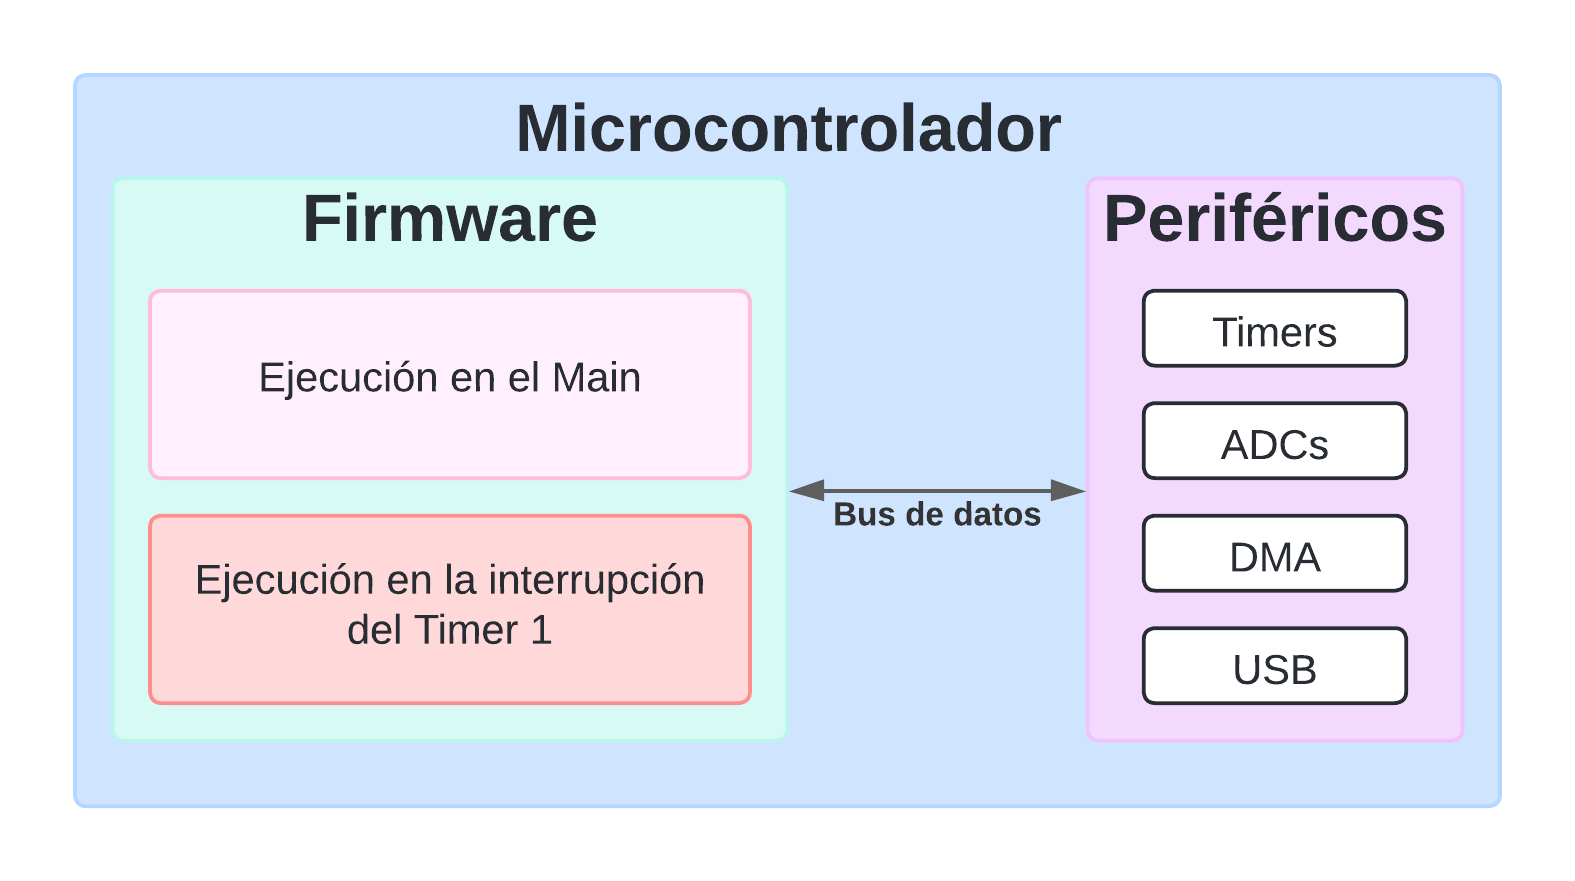
\includegraphics[width=0.8\textwidth]{imagenes/Diagramas/lineas de ejecucion.png}
	\caption{Bosquejo de la estructura general del firmware en el microcontrolador.}
	\label{firmware_microcontrolador}
\end{figure}
\FloatBarrier


\subsection{Ejecución en Main}

\begin{figure}[ht]
	\centering
	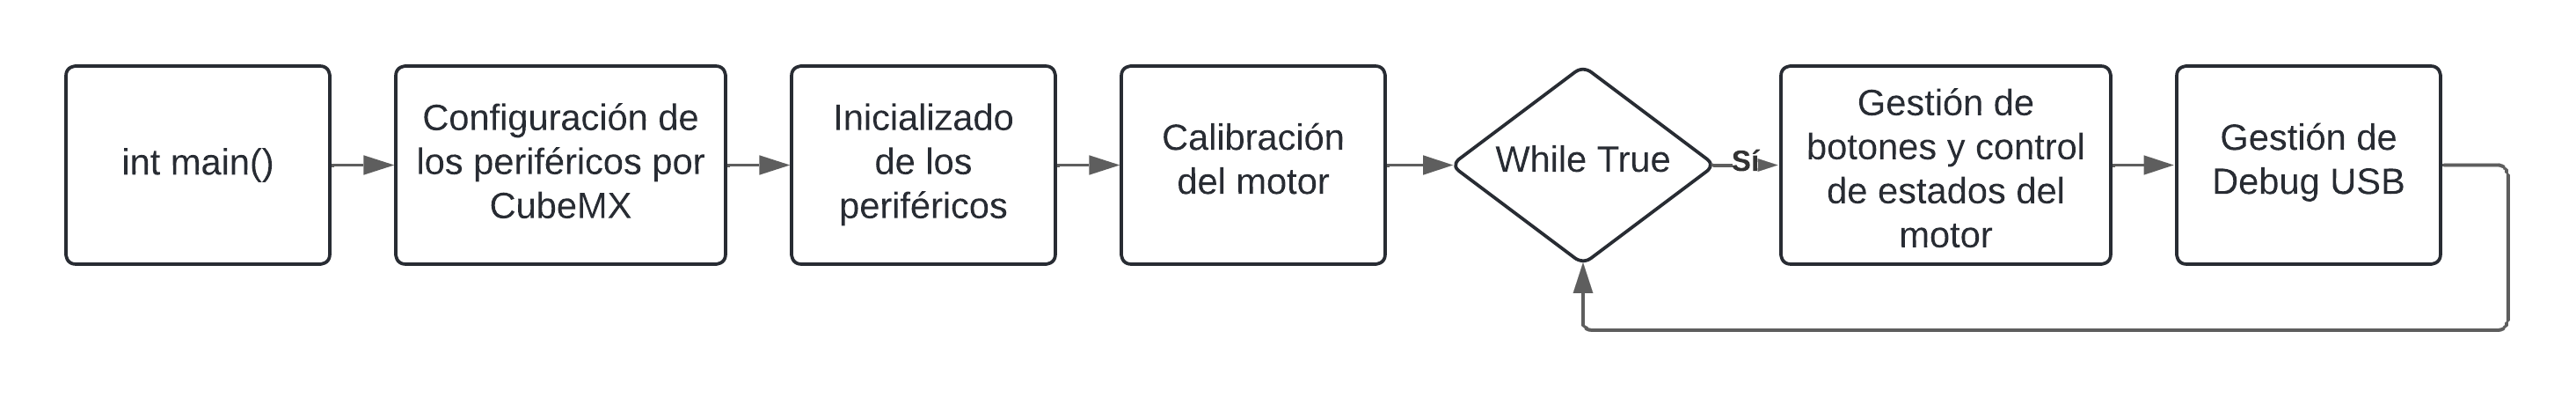
\includegraphics[width=\textwidth]{imagenes/Diagramas/linea main.png}
	\caption{Diagrama de flujo de las tareas principales en la línea de ejecución \texttt{main()}.}
	\label{fig:linea_ejecucion_main}
\end{figure}
\FloatBarrier

La ejecución en \texttt{main} inicia con una etapa de \textbf{configuración del sistema}, en la cual se inicializan los periféricos (por ejemplo, los \textbf{ADCs} y los \textbf{timers}). Posteriormente, se ejecuta una \textbf{secuencia de arranque del motor}, que incluye la calibración del cero en los sensores de corriente, el proceso de \emph{homing} y el ajuste del \emph{offset} en el motor.

\newpage
Completada esta configuración inicial, el sistema entra en un \textbf{bucle principal} que permite realizar distintas acciones, entre las cuales se encuentran:
\begin{itemize}
	\item Armado y desactivación del motor.
	\item Recalibration del motor.
	\item Control de los estados del motor.
	\item Envió de información por el USB.
\end{itemize}

\subsection{Ejecución en Interrupción}

\begin{figure}[ht]
	\centering
	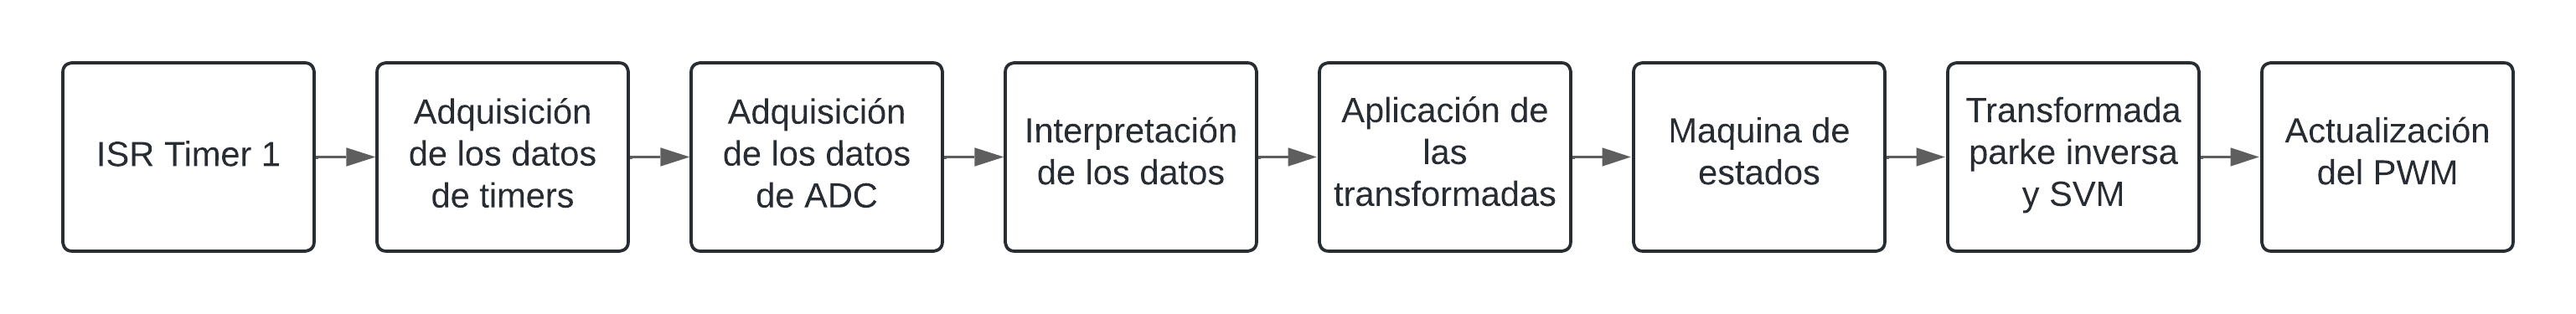
\includegraphics[width=\textwidth]{imagenes/Diagramas/linea timer.png}
	\caption{Diagrama de flujo de las tareas principales en la línea de ejecución de la interrupción.}
	\label{fig:linea_ejecucion_interrupcion}
\end{figure}
\FloatBarrier

La \textbf{rutina de interrupción} \href{https://www.youtube.com/watch?v=RJX_jYm8T84}{asociada} al \texttt{Timer 1} maneja el \textbf{lazo de control del motor} y se ejecuta a una frecuencia de 48 kHz. Su funcionamiento comienza con la obtención de datos provenientes de diversos periféricos, tales como:
\begin{itemize}
    \item Tiempos medidos por los \textbf{timers}.
    \item Posición del \textbf{encoder}.
    \item Lecturas de los \textbf{ADCs}.
\end{itemize}
En primer lugar, se \textbf{normalizan} los valores capturados para poder trabajar con estos desde valore reales. A continuación, se aplican las \textbf{transformadas de Clarke y Park} para obtener las variables de estado del motor. 

Posteriormente, una \textbf{máquina de estado} administra los diferentes modos de operación (por ejemplo, el retorno a \emph{home} o diversas configuraciones del lazo de control). Finalmente, los valores de salida de los \textbf{controladores PI} se transforman de nuevo mediante la inversa de Park y se emplea la \textbf{SVM} para calcular las señales de \emph{PWM} correspondientes..

\newpage
\section{Observaciones y posibles mejoras}

Durante el desarrollo del firmware, se identificó una consideración relevante para el sistema: la familia de microcontroladores STM32H7 presenta un error de arquitectura que complica el uso del DMA en condiciones normales. Este problema se debe a la división de la memoria RAM en regiones diferentes, lo que obliga a especificar la región de memoria deseada para cada variable o registro objetivo del DMA.

En lo que respecta al entorno de desarrollo, fue necesario emplear una máquina virtual con Ubuntu a través de WSL (Windows Subsystem for Linux) para compilar y escribir el código fuente utilizando VSCode, dado que la instalación del entorno en Windows no ofreció los resultados esperados.

En cuanto al lenguaje de programación, aunque el firmware se implementó en C, se observó que los microcontroladores STM32 también pueden ser programados en C++ con ligeras modificaciones al archivo \texttt{main}, lo que podría simplificar la gestión de recursos y la modularidad del código al permitir el uso de objetos.

Por último, para organizar de manera eficaz las subtareas y propiciar una mayor escalabilidad, se sugiere utilizar FreeRTOS. Este sistema operativo de tiempo real para microcontroladores puede integrarse directamente desde STM32CubeMX, proporcionando una estructura más robusta para el manejo de hilos de ejecución (threads) y facilitando la segmentación adecuada de las funciones que componen el firmware.

\newpage
\chapter{Validación}
Para las validaciones, se realizó una adquisición de datos, donde estos se recopilan ciclo a ciclo en la memoria RAM del microcontrolador para su posterior envío de forma asincrónica por el puerto USB, como se muestra en la figura \ref{flujo_debug}. Los datos son recibidos en una computadora a través de un código en Python, donde se almacenan en archivos CSV. Esta recopilación de información se realiza al final de cada ejecución de la interrupción del sistema, la cual se ejecuta a una frecuencia de 48 kHz. Debido a las limitaciones de memoria, la recopilación de datos solo puede llevarse a cabo durante un período de aproximadamente 100 ms, hasta alcanzar la capacidad máxima de la memoria.

\begin{figure}[ht]
	\centering
	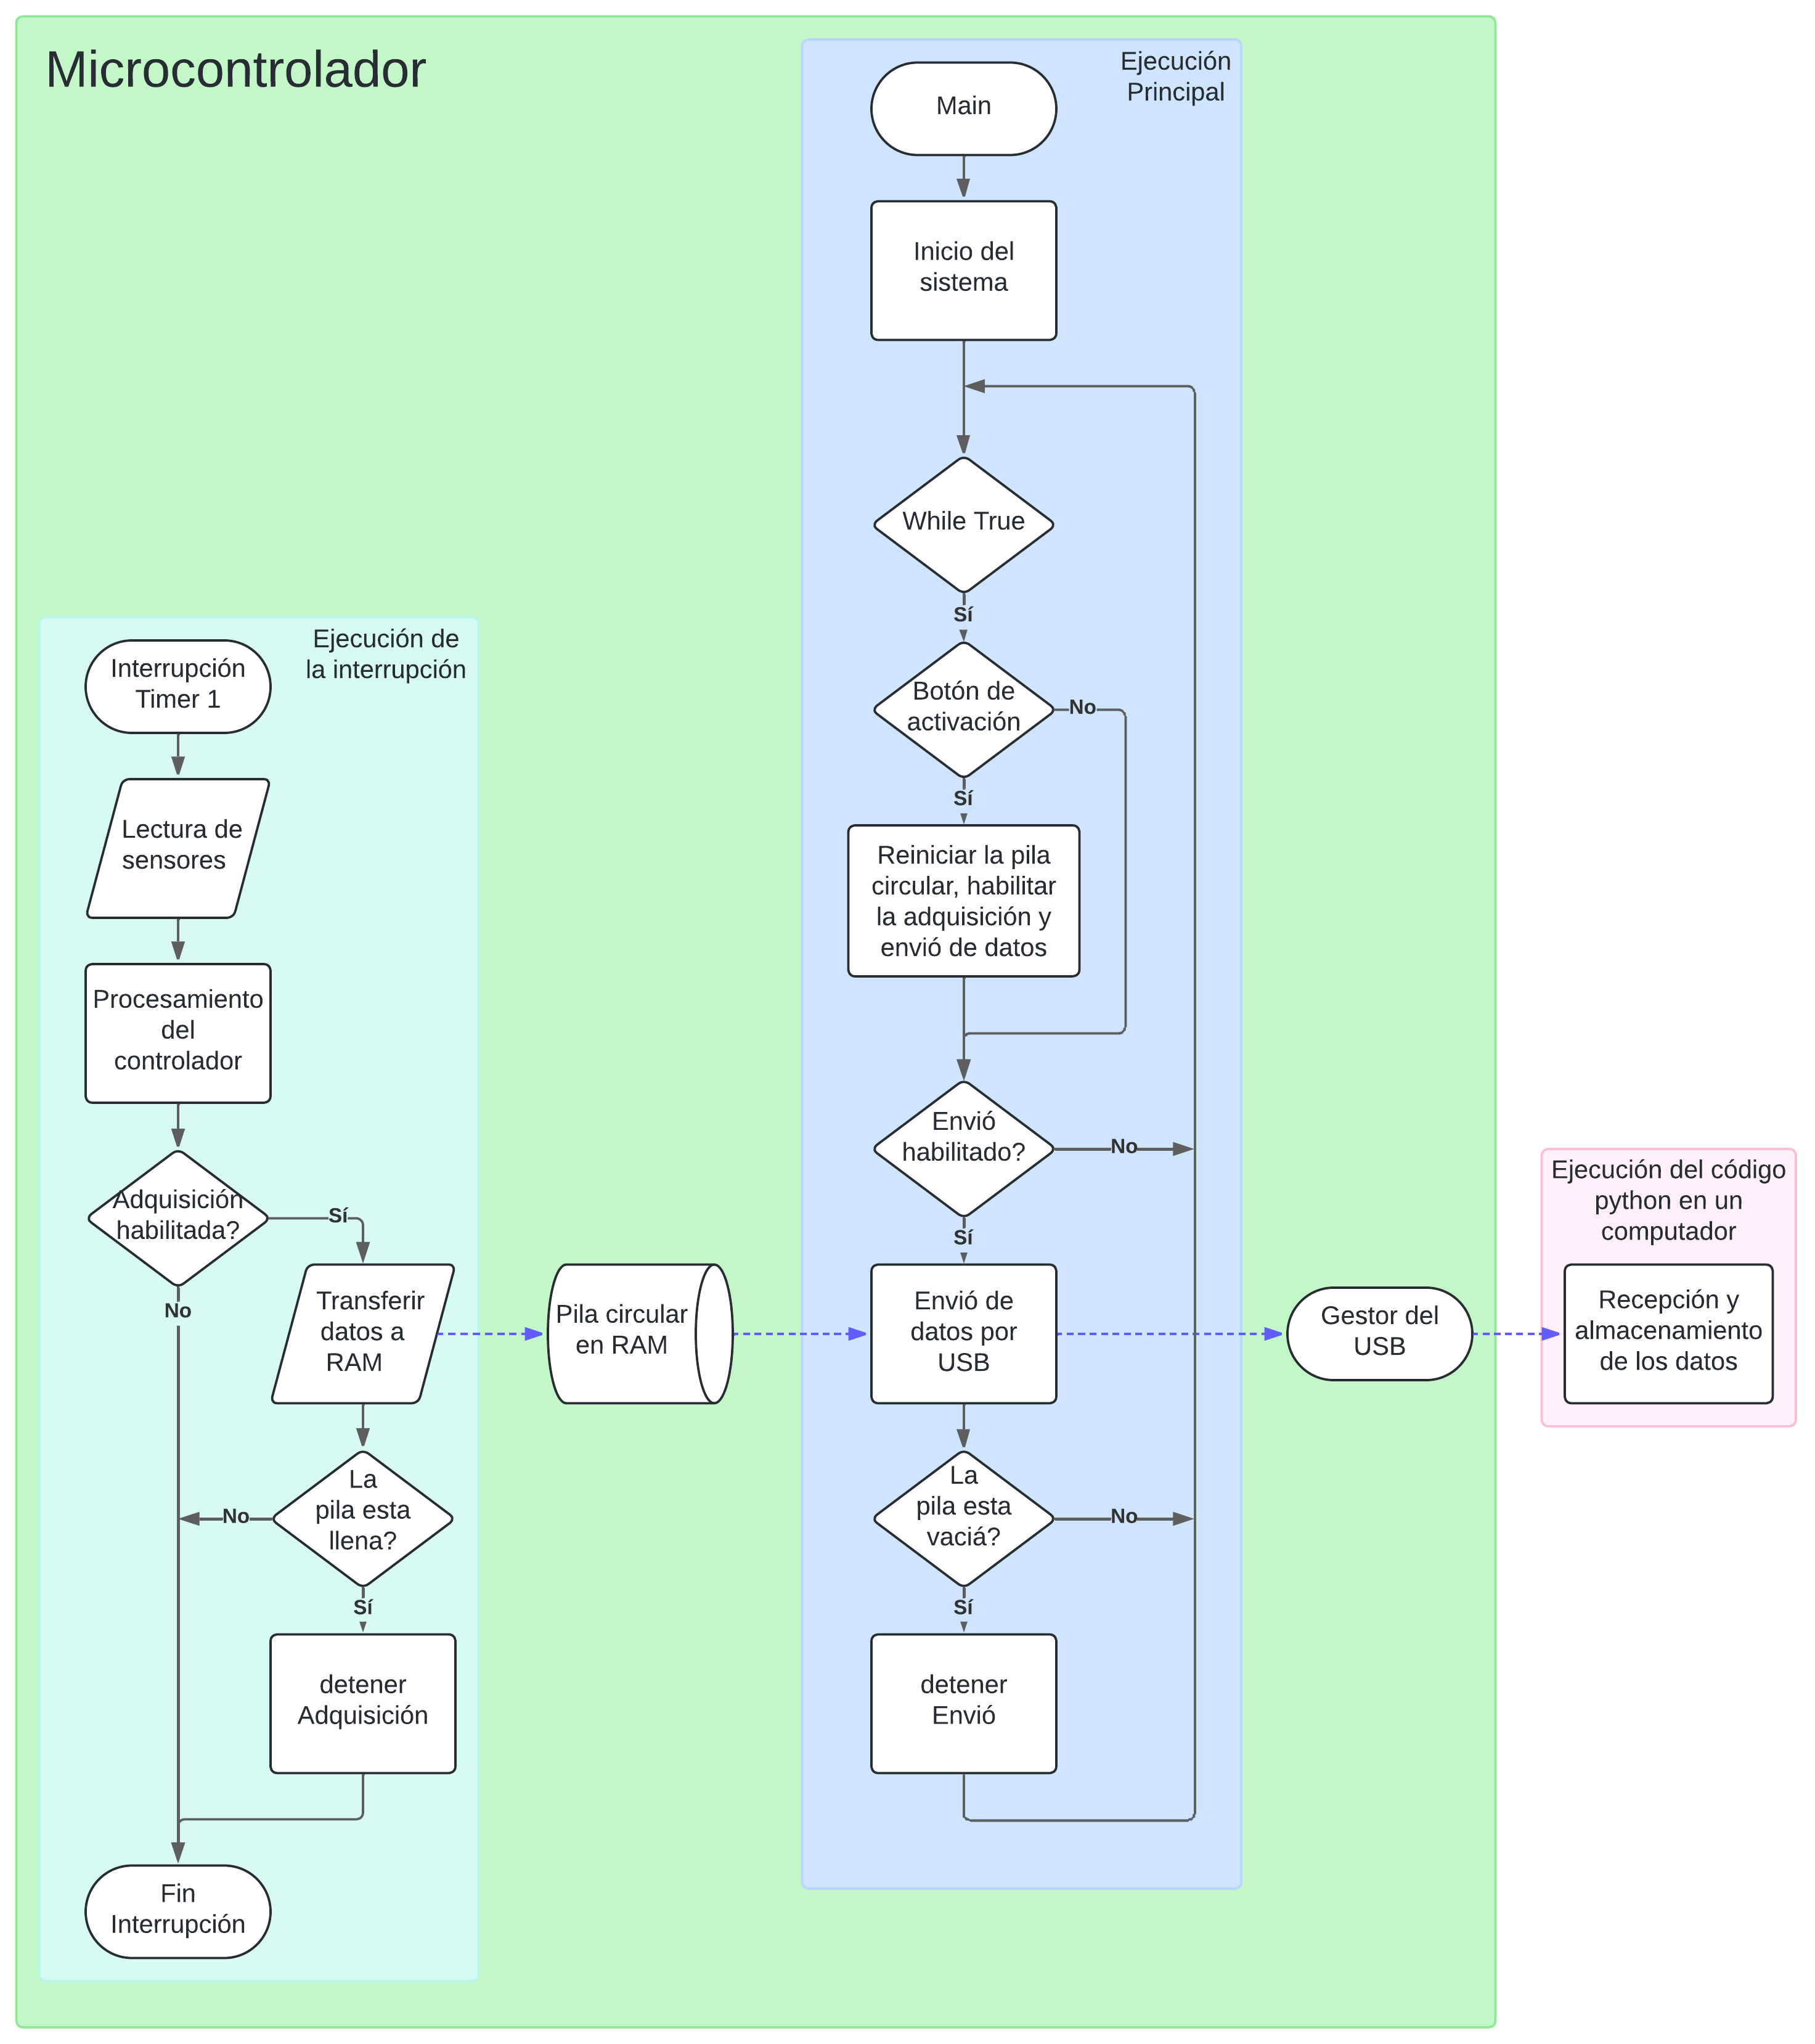
\includegraphics[width=0.76\textwidth]{imagenes/Diagramas/Debug USB.png}
	\caption{Diagrama de flujo adquisición de datos.}
	\label{flujo_debug}
\end{figure}
\FloatBarrier

\section{Validación de la adquisición y transformación de las mediciones de corriente}

\subsection{Validación de las mediciones de corriente}
Se validaran las mediciones de corriente adquiridas desde el microcontrolador.

\begin{figure}[ht]
	\centering
	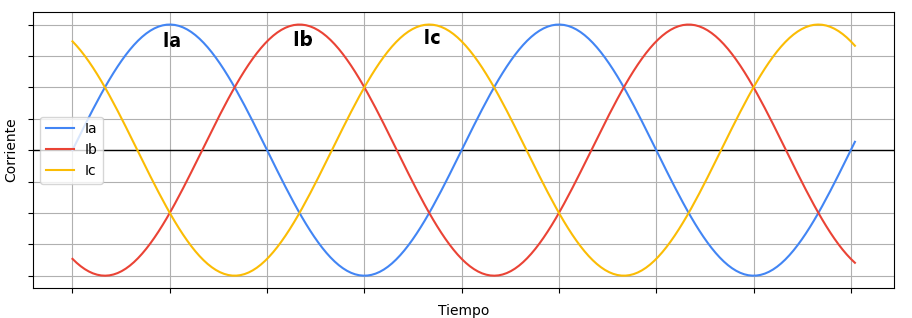
\includegraphics[width=0.8\textwidth]{imagenes/graficas/Corrientes_ABC_ideal.png}
	\caption{Corrientes ideales en un sistema trifásico equilibrado.}
	\label{corrientes_ABC_ideal}
\end{figure}
\FloatBarrier

En la figura \ref{corrientes_ABC_ideal} se representan las señales ideales de un sistema trifásico equilibrado, con las tres corrientes de fase $I_a$, $I_b$ e $I_c$, cada una de ellas con una forma senoidal pura y un desfase de $120^\circ$ entre sí.

\begin{figure}[ht]
	\centering
	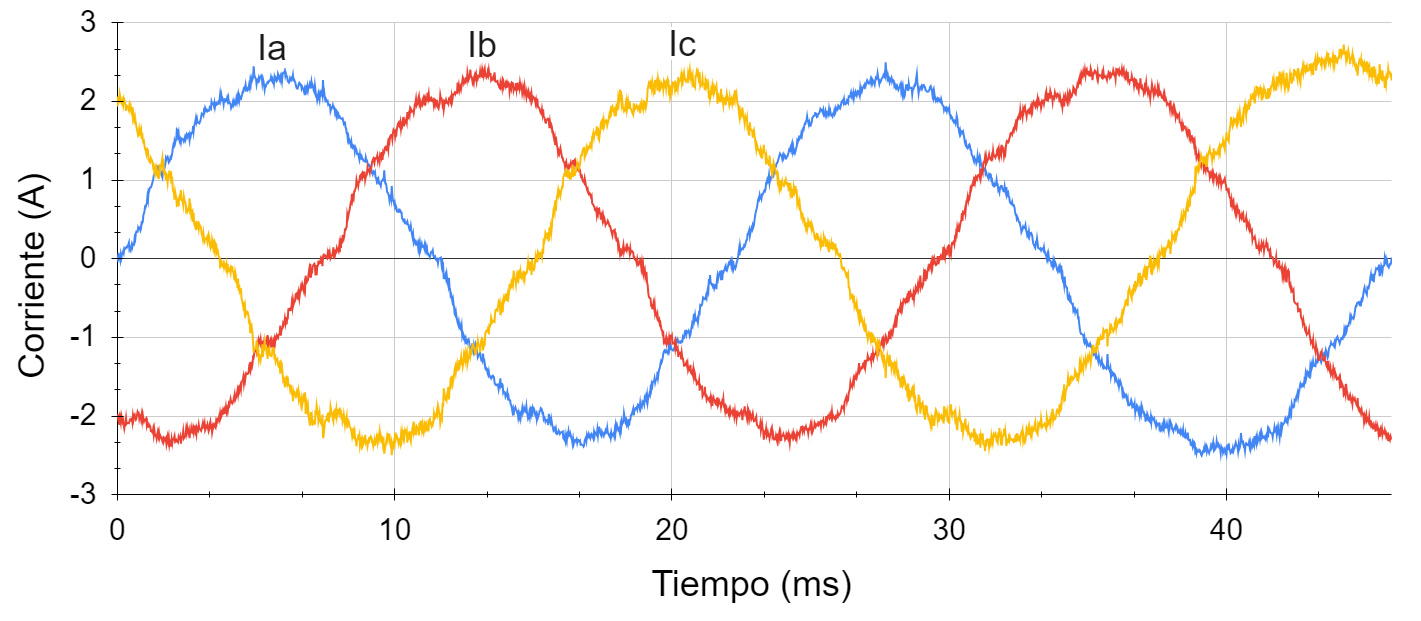
\includegraphics[width=0.8\textwidth]{imagenes/graficas/Corrientes_ABC.png}
	\caption{Corrientes medidas en el sistema trifásico.}
	\label{corrientes_ABC}
\end{figure}
\FloatBarrier

En la figura \ref{corrientes_ABC} se pueden apreciar las corrientes de fase, las cuales presentan una cantidad significativa de ruido, aun cuando internamente pasan por un filtro complementario con una frecuencia de corte $f_W=12000Hz$, pero mantienen un comportamiento sinusoidal con el desfase de $120^\circ$ entre señales, como es característico de un sistema trifásico equilibrado. pero la cantidad de ruido podría indicar que seria necesario disminuir la frecuencia de corte en el filtro complementario o agregar un filtro pasivo en el circuito.

\newpage
\subsection{Validación de la transformada de Clarke}

Se validara los resultado a la salida de la transformada de Clarke en el microcontrolador.

\begin{figure}[ht]
	\centering
	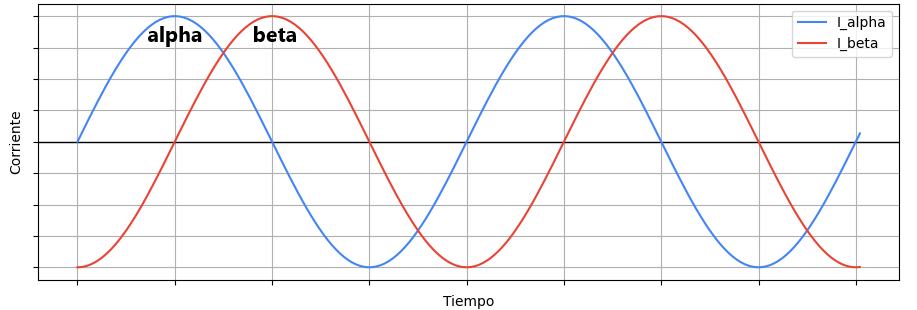
\includegraphics[width=0.8\textwidth]{imagenes/graficas/Corrientes_AlphaBeta_ideal.png}
	\caption{Corrientes ideales en el plano $\alpha\beta$.}
	\label{corrientes_alpha_beta_ideal}
\end{figure}
\FloatBarrier

En la figura \ref{corrientes_alpha_beta_ideal} se representan las corrientes ideales en el plano $\alpha\beta$, con las formas senoidales puras con un desfase de $90^\circ$ entre sí.

\begin{figure}[ht]
	\centering
	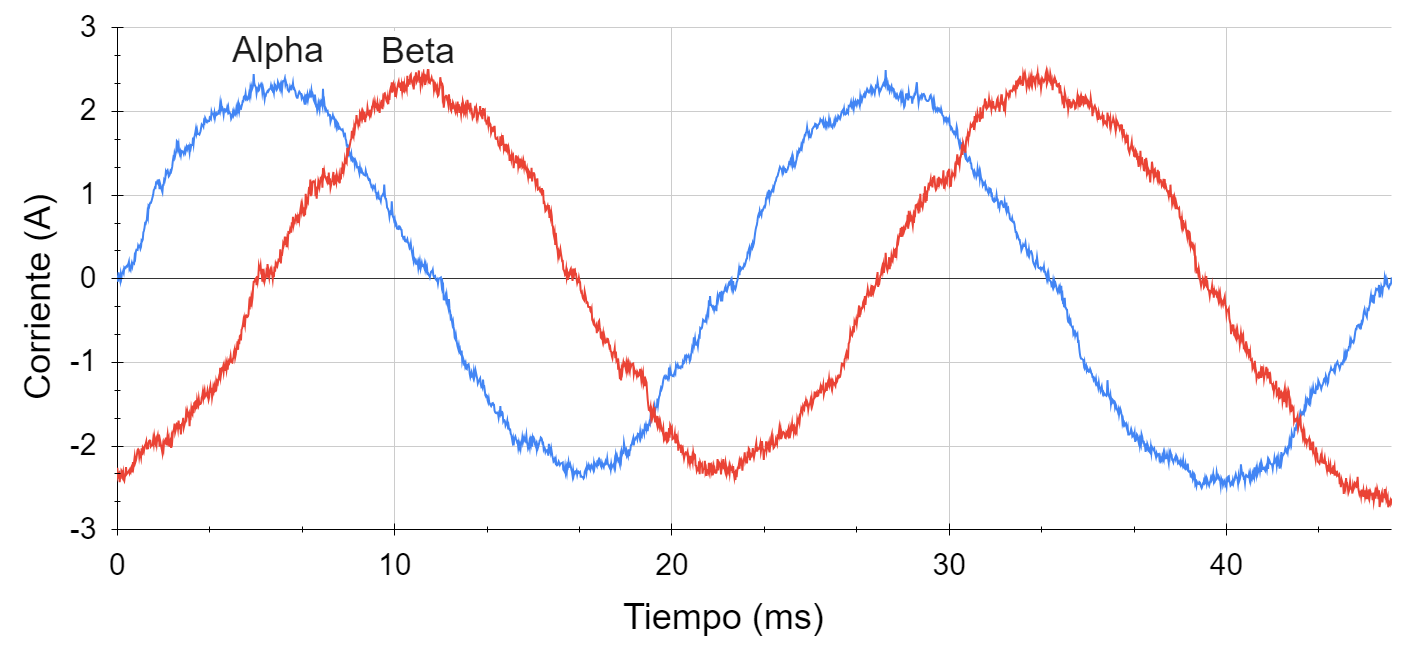
\includegraphics[width=0.8\textwidth]{imagenes/graficas/Corrientes_AlphaBeta.png}
	\caption{Corrientes medidas en el plano $\alpha\beta$.}
	\label{corrientes_alpha_beta}
\end{figure}
\FloatBarrier

En la figura \ref{corrientes_alpha_beta} se pueden apreciar como las corrientes $\alpha\beta$ reflejan el ruido presente en las mediciones de los sensores de corriente, pero mantienen un comportamiento esperado a la salida de la transformada de Clarke con las dos señales sinusoidal con el desfase de $90^\circ$ entre señales, como es característico.

\newpage
\subsection{Validación de la transformada de Park}

Se validara los resultado a la salida de la transformada de Park en el microcontrolador.

\begin{figure}[ht]
	\centering
	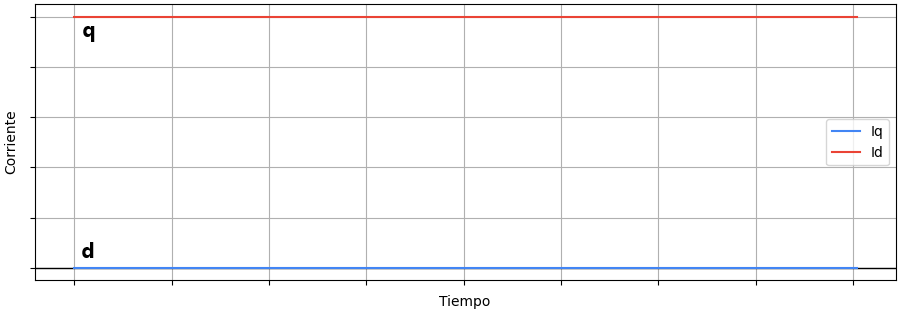
\includegraphics[width=0.8\textwidth]{imagenes/graficas/Corrientes_dq_ideal.png}
	\caption{Corrientes ideales en el plano $dq$.}
	\label{corrientes_dq_ideal}
\end{figure}
\FloatBarrier

En la figura \ref{corrientes_dq_ideal} se representan las corrientes ideales en el plano $dq$, donde lo ideal, es que la corriente directa tenga un valor de cero, para mantener la eficiencia del sistema, mientras que solo la corriente de cuadratura tiene un valor distinto a cero.

\begin{figure}[ht]
	\centering
	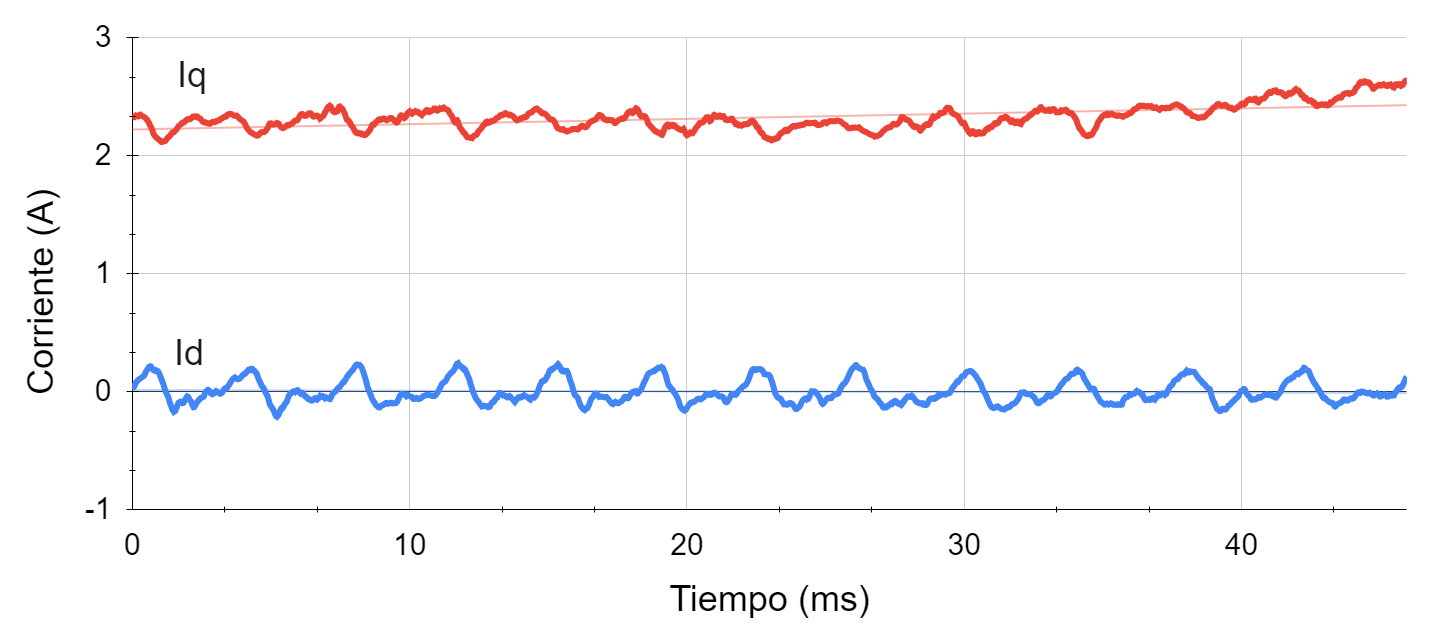
\includegraphics[width=0.8\textwidth]{imagenes/graficas/Corrientes_dq.png}
	\caption{Corrientes medidas en el plano $dq$.}
	\label{corrientes_dq}
\end{figure}
\FloatBarrier

En la figura \ref{corrientes_dq} se pueden apreciar como las corrientes $dq$ presenta una menor cantidad de ruido gracias a que su filtro complementario esta ajustado para una frecuencia de corte de $f_W=800Hz$, aunque igualmente presentan ciertas deformaciones y e inestabilidad con un patron aparentemente constante, pero en términos generales mantienen aproximadamente el comportamiento esperado a la salida de la transformada de Park.

\newpage
\section{Validación de los Controladores PI}
En esta validación se busca comprobar si los controladores PI de velocidad y corriente son capaces de mantener sus setpoints. Las pruebas se realizaron de forma estática, aplicando una carga ligera sobre el motor y capturando datos durante este proceso.

\subsection{Validación del controlador de velocidad}
Para la validación, se aplicó un setpoint de 116.8 RPM utilizando uno de los potenciómetros disponibles.

\begin{figure}[ht]
	\centering
	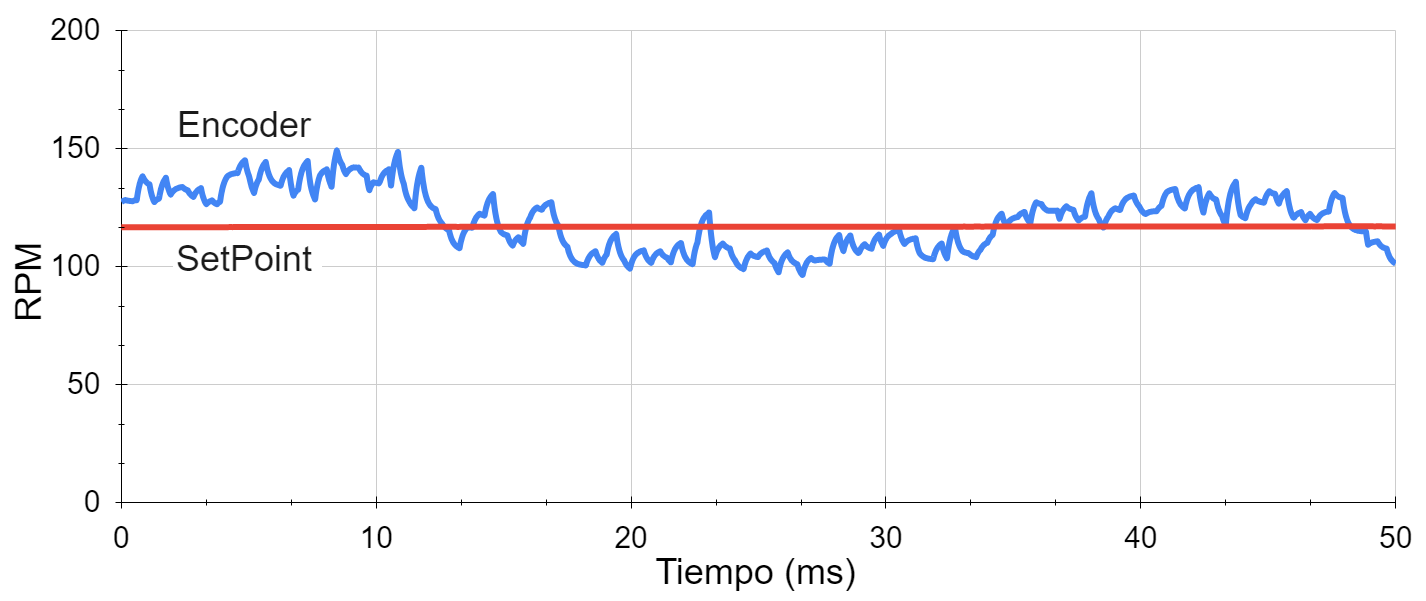
\includegraphics[width=0.8\textwidth]{imagenes/graficas/CV.png}
	\caption{Velocidad medida por el encoder y setpoint de velocidad.}
	\label{velocidad_encoder}
\end{figure}
\FloatBarrier

En la Figura \ref{velocidad_encoder}, se observa que la velocidad medida por el encoder sigue adecuadamente el setpoint establecido de 116.8 RPM. A pesar de ligeras oscilaciones, el controlador de velocidad mantiene el régimen deseado, \href{https://www.youtube.com/watch?v=B8VR5mQcgjI}{demostrando} su capacidad para alcanzar y mantener el setpoint bajo condiciones de carga estática.

\newpage
\subsection{Validación del controlador de corriente}

\begin{figure}[ht]
	\centering
	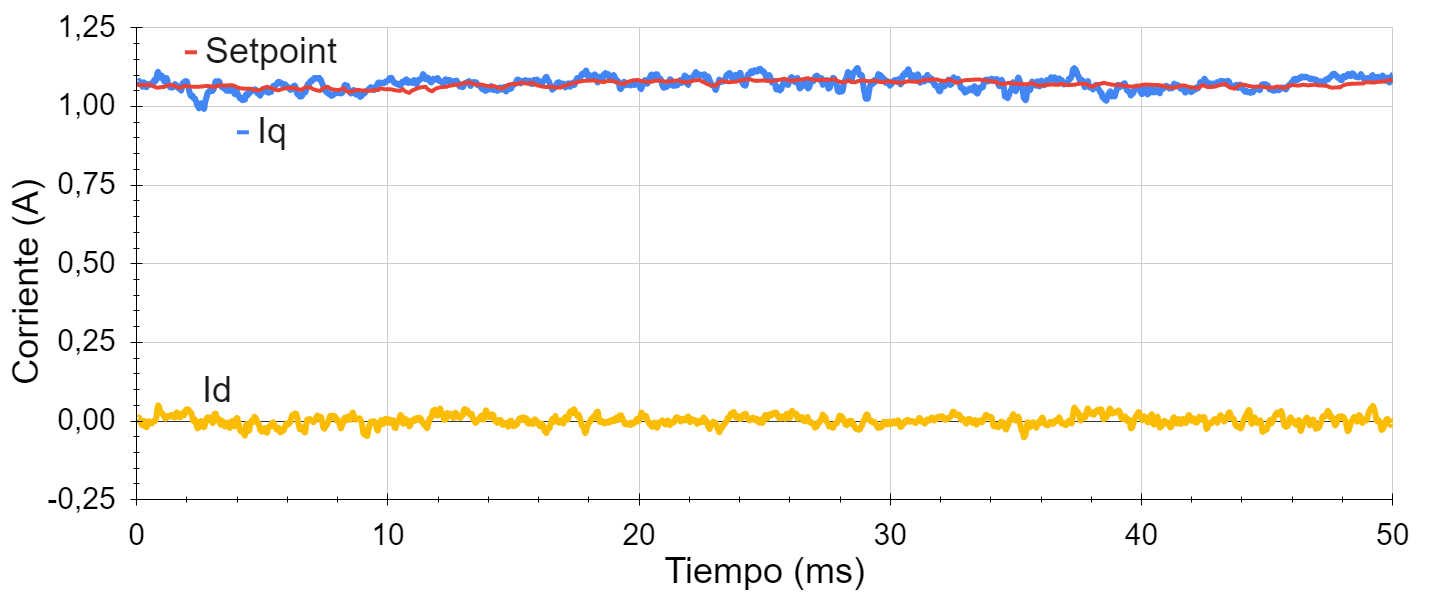
\includegraphics[width=0.8\textwidth]{imagenes/graficas/CV_CC.png}
	\caption{Corrientes medidas en el plano $dq$.}
	\label{cont_corrientes_dq}
\end{figure}
\FloatBarrier

Como se muestra en la Figura \ref{cont_corrientes_dq}, las corrientes en el plano $dq$ indican que el controlador de corriente logra mantener la corriente de cuadratura ($I_q$) cercana al valor de referencia proporcionado por el controlador de velocidad, mientras que la corriente directa ($I_d$) se mantiene próxima a cero. Esto evidencia que el controlador de corriente regula eficazmente las corrientes según los setpoints establecidos.

\begin{figure}[ht]
	\centering
	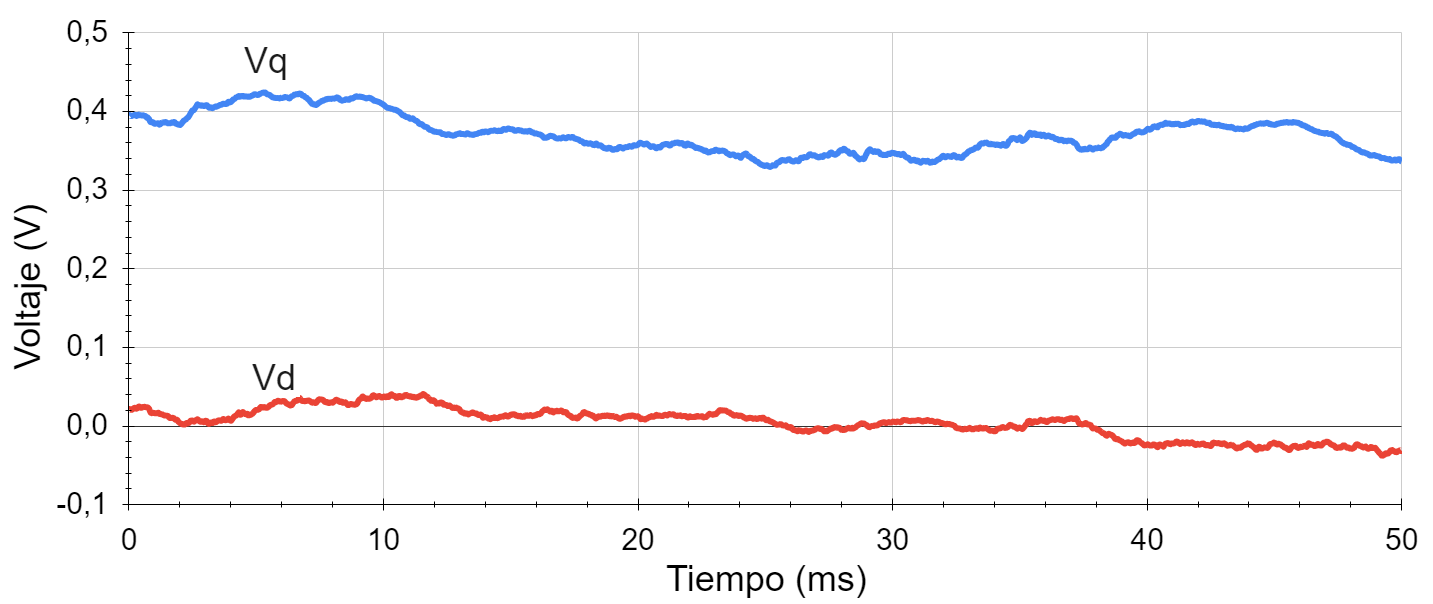
\includegraphics[width=0.8\textwidth]{imagenes/graficas/CC_DQ.png}
	\caption{Voltajes en el plano $dq$.}
	\label{voltajes_dq}
\end{figure}
\FloatBarrier

Además, la Figura \ref{voltajes_dq} presenta los voltajes en el plano $dq$, donde se aprecia que las tensiones generadas están dentro de los valores esperados para mantener las corrientes deseadas. Esto corrobora que el controlador de corriente responde adecuadamente a las demandas del sistema, contribuyendo al correcto desempeño del motor bajo condiciones de carga.

\newpage
\section{Validación señales del SVM}

Para validar el funcionamiento del modulador por vector espacial (SVM), se realizaron pruebas virtuales aplicando diferentes valores de tensión de referencia $V_{\text{ref}}$ al SVM para observar su comportamiento. Durante estas pruebas, se utilizó un analizador lógico para capturar las señales PWM generadas por el microcontrolador. En la captura presentada, se aisló un ciclo completo del PWM donde se puede apreciar de forma clara la secuencia de activación correspondiente al sector 1.

\begin{figure}[ht]
	\centering
	\includegraphics[width=0.9\textwidth]{imagenes/graficas/señales timer.png}
	\caption{Señales del timer.}
	\label{señal_timer}
\end{figure}
\FloatBarrier

En la Figura \ref{señal_timer}, se observan las señales PWM correspondientes a las tres fases generadas por el microcontrolador. La secuencia de activación muestra que el SVM implementado sigue correctamente el patrón teórico esperado para el sector 1, evidenciando una conmutación precisa y sincronizada de los transistores del inversor. Esto confirma que el SVM está modulando adecuadamente las señales PWM para generar los vectores de tensión requeridos.

\newpage
\chapter*{Comentarios y Conclusiones}
\addcontentsline{toc}{chapter}{Comentarios y Conclusiones}

\paragraph{Respecto al objetivo: ``Estudiar los principios del Control de Campo Orientado (FOC) y la modulación de espacio vectorial (SVM) para aplicarlos en el diseñó del controlador''} Se concluye que la base teórica relacionada con el funcionamiento de los motores \textit{brushless} y el Control de Campo Orientado (FOC) abarca un espectro más amplio que el revisado en este proyecto. Las transformadas de Clarke y Park simplifican el análisis e implementación del sistema, aunque sería posible profundizar en metodologías de control FOC directo.

\paragraph{Respecto al objetivo: ``Diseñar el hardware para el controlador FOC, con los componentes mínimos necesarios para validar el funcionamiento''} Se concluye que el uso de \emph{Autodesk Eagle} facilita de manera significativa el proceso de diseñó tanto del esquemático como de la placa de circuito impreso (PCB). La disponibilidad de recursos y librerías en línea agiliza la búsqueda de los componentes específicos y su integración, garantizando la coherencia entre el símbolo de cada dispositivo y su respectivo \emph{footprint}. Además, la compatibilidad con los servicios de \emph{JLCPCB}, la cual proporciona reglas de diseñó y formatos de archivos \emph{Gerber} precisos, contribuyó a la fabricación eficiente y libre de inconvenientes de la placa.

\paragraph{Respecto al objetivo: ``Configurar y programar el microcontrolador para el algoritmo FOC, utilizando las librerías HAL de STM32''} Se concluye que la utilización de \emph{STM32CubeMX} reduce de forma notable la complejidad inicial de configuración de los periféricos, puesto que automatiza gran parte del proceso y evita lidiar directamente con registros de bajo nivel y los usos avanzados de la biblioteca HAL. No obstante, el elevado número de módulos disponibles en la familia STM32H7 y la gran variedad de parámetros de configuración requirieron una curva de aprendizaje considerable para conseguir un ajuste óptimo. A pesar de ello, la configuración final aprovecha de manera significativa las prestaciones del microcontrolador.

\paragraph{Respecto al objetivo: ``Validar el funcionamiento del controlador y proponer posibles mejoras para su aplicación en robótica competitiva''} Se concluye que el controlador desarrollado exhibe un desempeño estable en condiciones normales de operación. Sin embargo, las pruebas evidenciaron dificultades cuando se exige al sistema con aceleraciones bruscas o cambios de dirección repentinos. Además, aunque las compuertas AND permiten deshabilitar con seguridad el puente MOSFET ante posibles fallas, persiste el inconveniente de doble activación (\emph{shoot-through}) en determinadas circunstancias, lo que puede comprometer la integridad del prototipo. Dichas observaciones confirman la necesidad de perfeccionar tanto el hardware como el firmware para afrontar escenarios de carga extrema.

\paragraph{Respecto al objetivo principal: ``Implementar un controlador de tipo FOC para motores \textit{brushless} con encoder, utilizando un microcontrolador STM32, que sirva de base para un driver especializado en la robótica competitiva''} Se concluye que el controlador constituye una solución \href{https://www.youtube.com/watch?v=XnAQtDEaI2I}{funcional} para requerimientos estándar y cumple con la finalidad de servir como base para un \emph{driver} especializado en robótica competitiva. A lo largo del documento, se sugieren mejoras potenciales en ambas vertientes hardware y firmware que podrían optimizar el comportamiento del sistema en condiciones extremas, habituales en competencias de robótica. Adicionalmente, el uso de la familia STM32, en particular de la serie H7, ofreció un rendimiento notable, aun considerando ciertas dificultades de arquitectura que surgieron durante la fase de desarrollo. En consecuencia, se confirma la versatilidad de estos dispositivos para aplicaciones de alto desempeño y se resalta su amplio margen de crecimiento en futuros desarrollos.

\section*{Trabajos Futuros}
\addcontentsline{toc}{chapter}{Trabajos Futuros}
\begin{itemize}
	\item \textbf{Refinar la gestión del \emph{deadtime}:} Emplear controladores de puerta con protecciones integradas o añadir lógica adicional para prevenir la doble activación (\emph{shoot-through}) y preservar la confiabilidad del puente MOSFET.

	\item \textbf{Ampliar la robustez en el hardware:} Aumentar el ancho de las pistas o soldar barras de cobre en la PCB para soportar mejor los picos de corriente, junto con el uso de materiales termorresistentes (PETG o ABS) en piezas críticas que tengan contacto directo con el motor.

	\item \textbf{Optimizar la ejecución del firmware:} Migrar el código a C++ e integrar FreeRTOS para aprovechar la programación orientada a objetos y el manejo de hilos, facilitando la escalabilidad y la organización de tareas concurrentes.

	\item \textbf{Mejorar el filtrado de la señal de corriente:} Reducir la frecuencia de corte del filtro o añadir etapas analógicas pasivas para minimizar el ruido en las mediciones, incrementando así la precisión en el lazo de control.

	\item \textbf{Aumentar la versatilidad del sistema:} Explorar el soporte a un segundo motor y ampliar la capacidad de adquisición de datos, permitiendo el desarrollo de múltiples ejes de control para aplicaciones robóticas de mayor complejidad.

	\item \textbf{Incorporar compensaciones de cogging torque:} Implementar algoritmos de calibración y compensación que disminuyan la vibración producida por el entrehierro, optimizando así la estabilidad de velocidad y el rendimiento general del motor.
\end{itemize}

\href{https://www.youtube.com/watch?v=2yJgwwDcgV8}{\phantom{ASDF--------------------ASDF}}

\newpage
\addcontentsline{toc}{chapter}{Bibliografía}
\printbibliography

%\newpage
%\addcontentsline{toc}{chapter}{Anexos}

%\newpage
%\chapter*{Anexo: Pinout del Microcontrolador}
%\addcontentsline{toc}{section}{Anexo: Pinout del Microcontrolado}

%\begin{figure}[ht]
%	\centering
%	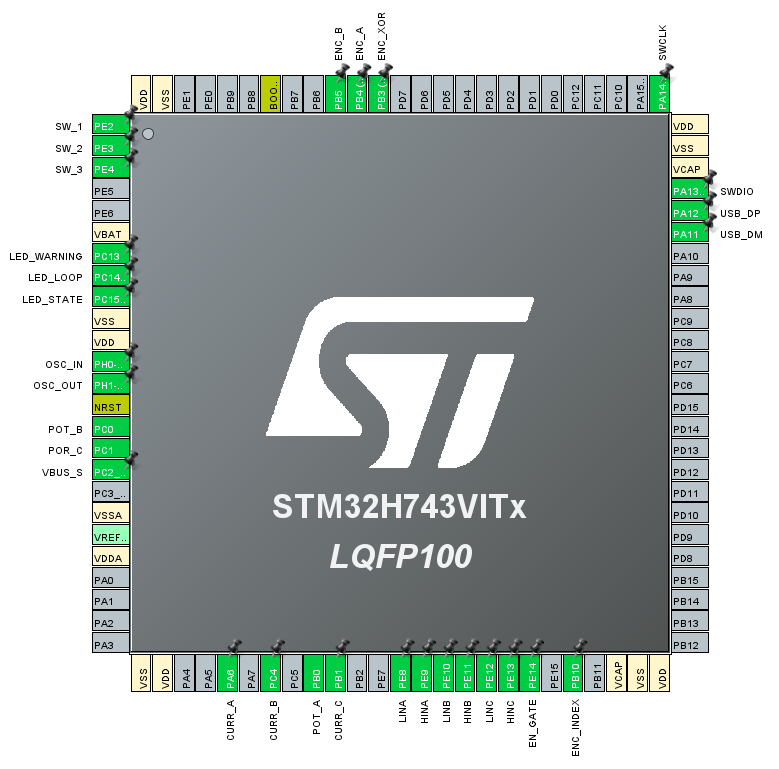
\includegraphics[width=\textwidth]{anexos/pinout.png}
%\end{figure}
%\FloatBarrier

%\newpage
%\chapter*{Anexo: Configuración RAM}
%\addcontentsline{toc}{section}{Anexo: Configuración RAM}

%\begin{figure}[ht]
%	\centering
%	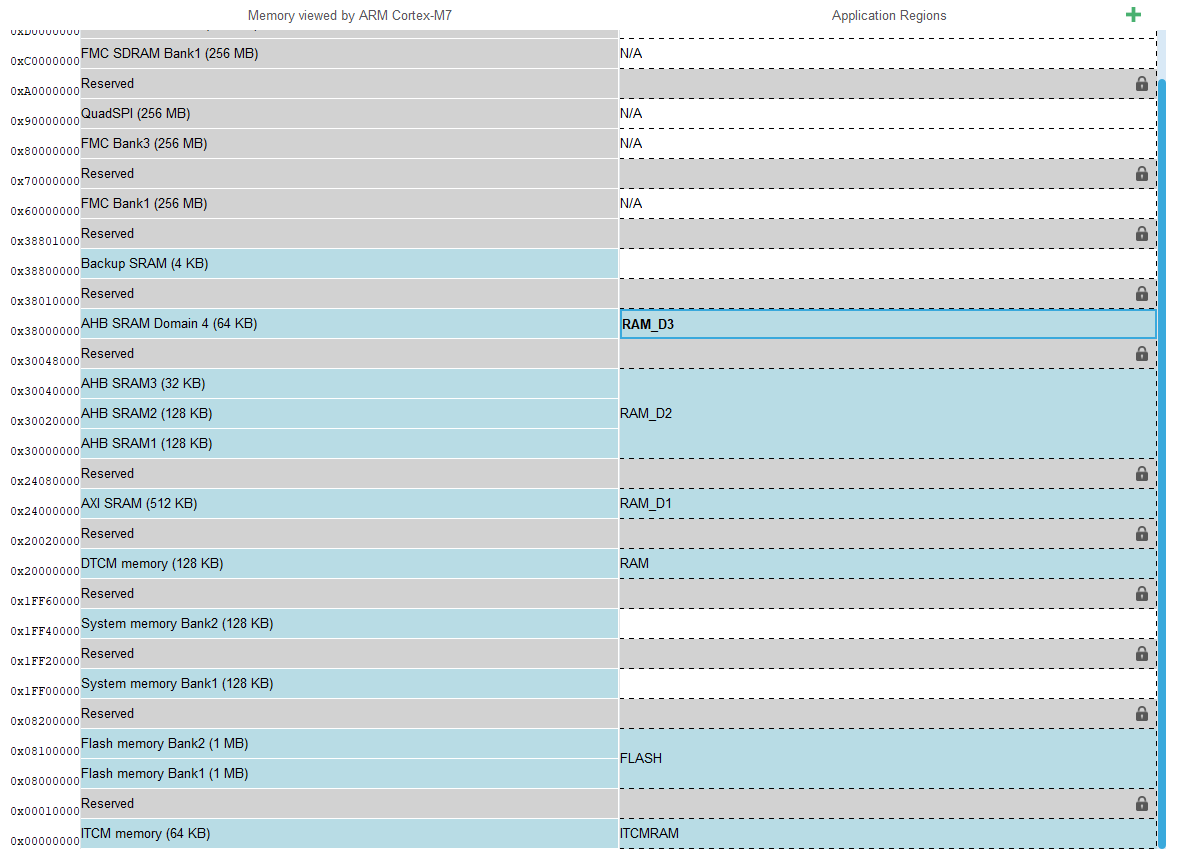
\includegraphics[width=\textwidth]{anexos/dominios RAM.png}
%\end{figure}
%\FloatBarrier

%\newpage
%\addcontentsline{toc}{section}{Anexo: Configuración Relojes}
%\includepdf[pages=-]{anexos/relojes.pdf}

\end{document}
